\documentclass[twoside]{book}

% Packages required by doxygen
\usepackage{fixltx2e}
\usepackage{calc}
\usepackage{doxygen}
\usepackage[export]{adjustbox} % also loads graphicx
\usepackage{graphicx}
\usepackage[utf8]{inputenc}
\usepackage{makeidx}
\usepackage{multicol}
\usepackage{multirow}
\PassOptionsToPackage{warn}{textcomp}
\usepackage{textcomp}
\usepackage[nointegrals]{wasysym}
\usepackage[table]{xcolor}

% Font selection
\usepackage[T1]{fontenc}
\usepackage[scaled=.90]{helvet}
\usepackage{courier}
\usepackage{amssymb}
\usepackage{sectsty}
\renewcommand{\familydefault}{\sfdefault}
\allsectionsfont{%
  \fontseries{bc}\selectfont%
  \color{darkgray}%
}
\renewcommand{\DoxyLabelFont}{%
  \fontseries{bc}\selectfont%
  \color{darkgray}%
}
\newcommand{\+}{\discretionary{\mbox{\scriptsize$\hookleftarrow$}}{}{}}

% Page & text layout
\usepackage{geometry}
\geometry{%
  a4paper,%
  top=2.5cm,%
  bottom=2.5cm,%
  left=2.5cm,%
  right=2.5cm%
}
\tolerance=750
\hfuzz=15pt
\hbadness=750
\setlength{\emergencystretch}{15pt}
\setlength{\parindent}{0cm}
\setlength{\parskip}{3ex plus 2ex minus 2ex}
\makeatletter
\renewcommand{\paragraph}{%
  \@startsection{paragraph}{4}{0ex}{-1.0ex}{1.0ex}{%
    \normalfont\normalsize\bfseries\SS@parafont%
  }%
}
\renewcommand{\subparagraph}{%
  \@startsection{subparagraph}{5}{0ex}{-1.0ex}{1.0ex}{%
    \normalfont\normalsize\bfseries\SS@subparafont%
  }%
}
\makeatother

% Headers & footers
\usepackage{fancyhdr}
\pagestyle{fancyplain}
\fancyhead[LE]{\fancyplain{}{\bfseries\thepage}}
\fancyhead[CE]{\fancyplain{}{}}
\fancyhead[RE]{\fancyplain{}{\bfseries\leftmark}}
\fancyhead[LO]{\fancyplain{}{\bfseries\rightmark}}
\fancyhead[CO]{\fancyplain{}{}}
\fancyhead[RO]{\fancyplain{}{\bfseries\thepage}}
\fancyfoot[LE]{\fancyplain{}{}}
\fancyfoot[CE]{\fancyplain{}{}}
\fancyfoot[RE]{\fancyplain{}{\bfseries\scriptsize Generated by Doxygen }}
\fancyfoot[LO]{\fancyplain{}{\bfseries\scriptsize Generated by Doxygen }}
\fancyfoot[CO]{\fancyplain{}{}}
\fancyfoot[RO]{\fancyplain{}{}}
\renewcommand{\footrulewidth}{0.4pt}
\renewcommand{\chaptermark}[1]{%
  \markboth{#1}{}%
}
\renewcommand{\sectionmark}[1]{%
  \markright{\thesection\ #1}%
}

% Indices & bibliography
\usepackage{natbib}
\usepackage[titles]{tocloft}
\setcounter{tocdepth}{3}
\setcounter{secnumdepth}{5}
\makeindex

% Hyperlinks (required, but should be loaded last)
\usepackage{ifpdf}
\ifpdf
  \usepackage[pdftex,pagebackref=true]{hyperref}
\else
  \usepackage[ps2pdf,pagebackref=true]{hyperref}
\fi
\hypersetup{%
  colorlinks=true,%
  linkcolor=blue,%
  citecolor=blue,%
  unicode%
}

% Custom commands
\newcommand{\clearemptydoublepage}{%
  \newpage{\pagestyle{empty}\cleardoublepage}%
}

\usepackage{caption}
\captionsetup{labelsep=space,justification=centering,font={bf},singlelinecheck=off,skip=4pt,position=top}

%===== C O N T E N T S =====

\begin{document}

% Titlepage & ToC
\hypersetup{pageanchor=false,
             bookmarksnumbered=true,
             pdfencoding=unicode
            }
\pagenumbering{alph}
\begin{titlepage}
\vspace*{7cm}
\begin{center}%
{\Large D\+S2482-\/\+RK }\\
\vspace*{1cm}
{\large Generated by Doxygen 1.8.14}\\
\end{center}
\end{titlepage}
\clearemptydoublepage
\pagenumbering{roman}
\tableofcontents
\clearemptydoublepage
\pagenumbering{arabic}
\hypersetup{pageanchor=true}

%--- Begin generated contents ---
\chapter{D\+S2482 Library}
\label{index}\hypertarget{index}{}The \mbox{\hyperlink{class_d_s2482}{D\+S2482}} is an I2C to 1-\/wire interface chip. It comes in two versions, the D\+S2482-\/100 (1-\/port) and D\+S2482-\/800 (8-\/port). Using an interface chip is helpful because most D\+S18\+B20/1-\/wire libraries use timing sensitive code and may run for extended periods with interrupts disabled. This can cause the rest of your program to have poor performance.

The library fully supports both single-\/drop and multi-\/drop modes, allowing many D\+S18\+B20 sensors on a single 1-\/wire bus.

The \mbox{\hyperlink{class_d_s2482}{D\+S2482}} library is completely asynchronous, never blocking for more than the time to do an I2C read or write. Interrupts are never disabled.

Every call uses a C++11 lambda completion handler. The second part of this document has a bit of explanation of why and how it works.

The \mbox{\hyperlink{class_d_s2482}{D\+S2482}} also has an internal transistor to pull the 1-\/wire bus high during temperature conversion and flash writes. This allows the use of parasitic power mode, requiring only two wires for sensors (DQ and G\+ND), with no separate power line. The library supports this as well.

\subsection*{Common tasks}

\subsubsection*{Get temperature of one sensor (single-\/drop)}


\begin{DoxyCode}
#include "DS2482.h"

SerialLogHandler logHandler;

DS2482 ds(Wire, 3);

const unsigned long CHECK\_PERIOD = 30000;
unsigned long lastCheck = 5000 - CHECK\_PERIOD;

void setup() \{
    Serial.begin(9600);
    ds.setup();

    DS2482DeviceReset::run(ds, [](DS2482DeviceReset&, int status) \{
        Serial.printlnf("deviceReset=%d", status);
    \});

    Serial.println("setup complete");
\}



void loop() \{

    ds.loop();

    if (millis() - lastCheck >= CHECK\_PERIOD) \{
        lastCheck = millis();

        // For single-drop you can pass an empty address to get the temperature of the only
        // sensor on the 1-wire bus
        DS24821WireAddress addr;

        DS2482GetTemperatureCommand::run(ds, addr, [](DS2482GetTemperatureCommand&, int status, float
       tempC) \{
            if (status == DS2482Command::RESULT\_DONE) \{
                char buf[32];
                snprintf(buf, sizeof(buf), "%.4f", tempC);

                Serial.printlnf("temperature=%s deg C", buf);
                Particle.publish("temperature", buf, PRIVATE);
            \}
            else \{
                Serial.printlnf("DS2482GetTemperatureCommand failed status=%d", status);
            \}
        \});
    \}
\}
\end{DoxyCode}


\subsubsection*{Get temperatures of multiple sensors (multi-\/drop)}


\begin{DoxyCode}
#include "DS2482.h"

SerialLogHandler logHandler;

DS2482 ds(Wire, 3);

DS2482DeviceListStatic<10> deviceList;
const unsigned long CHECK\_PERIOD = 30000;
unsigned long lastCheck = 10000 - CHECK\_PERIOD;

void setup() \{
    Serial.begin(9600);
    ds.setup();

    DS2482DeviceReset::run(ds, [](DS2482DeviceReset&, int status) \{
        Serial.printlnf("deviceReset=%d", status);
        DS2482SearchBusCommand::run(ds, deviceList, [](DS2482SearchBusCommand &obj, int status) \{

            if (status != DS2482Command::RESULT\_DONE) \{
                Serial.printlnf("DS2482SearchBusCommand status=%d", status);
                return;
            \}

            Serial.printlnf("Found %u devices", deviceList.getDeviceCount());
        \});
    \});

    Serial.println("setup complete");
\}


void loop() \{

    ds.loop();

    if (millis() - lastCheck >= CHECK\_PERIOD) \{
        lastCheck = millis();

        if (deviceList.getDeviceCount() > 0) \{

            DS2482GetTemperatureForListCommand::run(ds, deviceList, [](DS2482GetTemperatureForListCommand&,
       int status, DS2482DeviceList &deviceList) \{
                if (status != DS2482Command::RESULT\_DONE) \{
                    Serial.printlnf("DS2482GetTemperatureForListCommand status=%d", status);
                    return;
                \}

                Serial.printlnf("got temperatures!");

                for(size\_t ii = 0; ii < deviceList.getDeviceCount(); ii++) \{
                    Serial.printlnf("%s valid=%d C=%f F=%f",
                            deviceList.getAddressByIndex(ii).toString().c\_str(),
                            deviceList.getDeviceByIndex(ii).getValid(),
                            deviceList.getDeviceByIndex(ii).getTemperatureC(),
                            deviceList.getDeviceByIndex(ii).getTemperatureF());
                \}

            \});
        \}
        else \{
            Serial.printlnf("no devices found");
        \}
    \}
\}
\end{DoxyCode}


\subsubsection*{Multi-\/drop with parasitic power}

Just as the previous example, except within loop the call to D2482\+Get\+Temperature\+List\+Command\+::run has an extra optional fluent parameter, {\ttfamily .with\+Parasitic\+Power()}.


\begin{DoxyCode}
DS2482GetTemperatureForListCommand::run(ds, deviceList, [](DS2482GetTemperatureForListCommand&, int status,
       DS2482DeviceList &deviceList) \{
    if (status != DS2482Command::RESULT\_DONE) \{
        Serial.printlnf("DS2482GetTemperatureForListCommand status=%d", status);
        return;
    \}

    Serial.printlnf("got temperatures!");

    for(size\_t ii = 0; ii < deviceList.getDeviceCount(); ii++) \{
        Serial.printlnf("%s valid=%d C=%f F=%f",
                deviceList.getAddressByIndex(ii).toString().c\_str(),
                deviceList.getDeviceByIndex(ii).getValid(),
                deviceList.getDeviceByIndex(ii).getTemperatureC(),
                deviceList.getDeviceByIndex(ii).getTemperatureF());
    \}

\}).withParasiticPower();
\end{DoxyCode}


\subsubsection*{Multi-\/drop with J\+S\+ON publish}

This example is like the previous, except it publishes multiple sensor values via a single Particle.\+publish in J\+S\+ON format (up to 10 D\+S18\+B20s supported).


\begin{DoxyCode}
#include "DS2482.h"
#include "JsonParserGeneratorRK.h"

SerialLogHandler logHandler;

DS2482 ds(Wire, 3);

DS2482DeviceListStatic<10> deviceList;
JsonWriterStatic<256> jsonWriter;

const unsigned long CHECK\_PERIOD = 30000;
unsigned long lastCheck = 10000 - CHECK\_PERIOD;

void setup() \{
    Serial.begin(9600);
    ds.setup();

    DS2482DeviceReset::run(ds, [](DS2482DeviceReset&, int status) \{
        Serial.printlnf("deviceReset=%d", status);
        DS2482SearchBusCommand::run(ds, deviceList, [](DS2482SearchBusCommand &obj, int status) \{

            if (status != DS2482Command::RESULT\_DONE) \{
                Serial.printlnf("DS2482SearchBusCommand status=%d", status);
                return;
            \}

            Serial.printlnf("Found %u devices", deviceList.getDeviceCount());
        \});
    \});

    Serial.println("setup complete");
\}


void loop() \{

    ds.loop();

    if (millis() - lastCheck >= CHECK\_PERIOD) \{
        lastCheck = millis();

        if (deviceList.getDeviceCount() > 0) \{

            DS2482GetTemperatureForListCommand::run(ds, deviceList, [](DS2482GetTemperatureForListCommand&,
       int status, DS2482DeviceList &deviceList) \{
                if (status != DS2482Command::RESULT\_DONE) \{
                    Serial.printlnf("DS2482GetTemperatureForListCommand status=%d", status);
                    return;
                \}

                Serial.printlnf("got temperatures!");

                // Initialize the JsonWriter object and sets it to send 2 decimal places
                jsonWriter.init();
                jsonWriter.setFloatPlaces(2);

                // startObject is for the outer object and must be balanced with finishObjectOrArray.
                jsonWriter.startObject();

                // Write the actual temperatures
                for(size\_t ii = 0; ii < deviceList.getDeviceCount(); ii++) \{
                    if (deviceList.getDeviceByIndex(ii).getValid()) \{
                        // This creates a key of the form "t0" for the first, "t1" for the second, ...
                        char key[4];
                        key[0] = 't';
                        key[1] = '0' + ii;
                        key[2] = 0;

                        // Inserts the float as a key value pair
                        jsonWriter.insertKeyValue(key, deviceList.getDeviceByIndex(ii).getTemperatureC());
                    \}
                \}

                jsonWriter.finishObjectOrArray();

                Serial.println(jsonWriter.getBuffer());
                Particle.publish("temperature", jsonWriter.getBuffer(), PRIVATE);

                // Example output:
                // \{"t0":23.56,"t1":23.12\}
            \});
        \}
        else \{
            Serial.printlnf("no devices found");
        \}
    \}
\}
\end{DoxyCode}


Example serial output\+:


\begin{DoxyCode}
got temperatures!
\{"t0":23.56,"t1":23.12\}
\end{DoxyCode}


Because the 1-\/wire bus search is deterministic, it will always returns the sensors in the same order, sorted by 1-\/wire device address (increasing).

\subsection*{About lambdas, fluent-\/style and more}

The \mbox{\hyperlink{class_d_s2482}{D\+S2482}} library uses a C++11 style of coding that is very powerful, but will probably be foreign to you if you learned old-\/school C and C++. It\textquotesingle{}s actually more like the way Javascript/node.\+js is programmed.

One of the main advantages of the \mbox{\hyperlink{class_d_s2482}{D\+S2482}} library is that it\textquotesingle{}s completely asynchronous. No call blocks for more than the time it takes to make an I2C transfer. This is important because getting a temperature sensor reading can take 750 milliseconds, and most D\+S18\+B20 software libraries block during conversion.

\subsubsection*{Synchronous way}

Using the \href{https://build.particle.io/libs/DS18B20/0.1.7/tab/DS18B20.cpp}{\tt D\+S18\+B20 library}, you make a call like this\+:


\begin{DoxyCode}
float tempC = ds.getTemperature(addr);
\end{DoxyCode}


The main loop thread is blocked during this call for 750 milliseconds, which may affect performance elsewhere in your code.

\subsubsection*{State machines}

One common way of implementing asynchronous code is state machines. This is a bit of pseudo-\/code of what a state machine version might look like.


\begin{DoxyCode}
void loop() \{
    switch(state) \{
    case GET\_TEMPERATURE\_STATE:
        ds.startTemperature();
        state = TEMPERATURE\_WAIT\_STATE;
        break;

    case TEMPERATURE\_WAIT\_STATE:
        if (ds.isTemperatureDone()) \{
            float temp = ds.readTemperature();
            state = ANOTHER\_STATE;
        \}
        break;
    \}
\}
\end{DoxyCode}


State machines are really powerful, and actually how the \mbox{\hyperlink{class_d_s2482}{D\+S2482}} library is implemented internally, but can get a bit unwieldy.

\subsubsection*{Callbacks}

Callback functions are another common way of handling asynchronous code, like in this pseudo-\/code example\+:


\begin{DoxyCode}
void temperatureCallback(float temp) \{
    Serial.printlnf("got temperature %f", temp);
\}

void loop() \{
    if (millis() - lastCheck >= CHECK\_PERIOD) \{
        lastCheck = millis();
        ds.getTemperature(temperatureCallback);
    \}
\}
\end{DoxyCode}


The problem with callbacks is that it\textquotesingle{}s a pain to pass state data to the callback, and it requires some effort to make a callback handler a class member function.

\subsubsection*{The Lambda}

The lambda solves some of the problems with callbacks. Here\textquotesingle{}s an example of doing an asynchronous device reset call\+:


\begin{DoxyCode}
void setup() \{
    Serial.begin(9600);
    ds.setup();

    DS2482DeviceReset::run(ds, [](DS2482DeviceReset&, int status) \{
        Serial.printlnf("deviceReset=%d", status);
    \});

    Serial.println("setup complete");
\}
\end{DoxyCode}


The syntax is a little weird, and I\textquotesingle{}ll get to that a moment, however the important thing is that this block of code, the lambda, is executed later.


\begin{DoxyCode}
[](DS2482DeviceReset&, int status) \{
    Serial.printlnf("deviceReset=%d", status);
\}
\end{DoxyCode}


The


\begin{DoxyCode}
setup complete
\end{DoxyCode}


message appears next.

When the asynchronous device reset completes, the block runs and


\begin{DoxyCode}
deviceReset=1
\end{DoxyCode}


will likely be printed to the serial console. Note, however, that the lines after the block, like printing setup complete! won\textquotesingle{}t happen a second time.

A declaration of a lambda function looks like


\begin{DoxyCode}
[](DS2482DeviceReset&, int status) \{
    // Code goes here
\}
\end{DoxyCode}


The {\ttfamily \mbox{[}\mbox{]}} part is the capture, which we\textquotesingle{}ll discuss in a moment, and {\ttfamily (\mbox{\hyperlink{class_d_s2482_device_reset}{D\+S2482\+Device\+Reset}}\&, int status)} is a function parameter declaration. Basically the callback is a function that takes two parameters, a {\ttfamily \mbox{\hyperlink{class_d_s2482_device_reset}{D\+S2482\+Device\+Reset}}\&} object (not used here) and an {\ttfamily int status} (for status).

\subsubsection*{Nesting calls}

This example demonstrates two handy things\+:


\begin{DoxyItemize}
\item Making your lambda be a class member
\item Nesting lambdas for sequential operations
\end{DoxyItemize}


\begin{DoxyCode}
void TestClass::check() \{
    DS2482SearchBusCommand::run(ds, deviceList, [this](DS2482SearchBusCommand &obj, int status) \{

        if (status != DS2482Command::RESULT\_DONE) \{
            Serial.printlnf("DS2482SearchBusCommand status=%d", status);
            return;
        \}

        if (deviceList.getDeviceCount() == 0) \{
            Serial.println("no devices");
            return;
        \}

        DS2482GetTemperatureForListCommand::run(ds, obj.getDeviceList(),
       [this](DS2482GetTemperatureForListCommand&, int status, DS2482DeviceList &deviceList) \{
            if (status != DS2482Command::RESULT\_DONE) \{
                Serial.printlnf("DS2482GetTemperatureForListCommand status=%d", status);
                return;
            \}

            Serial.printlnf("got temperatures!");

            for(size\_t ii = 0; ii < deviceList.getDeviceCount(); ii++) \{
                Serial.printlnf("%s valid=%d C=%f F=%f",
                        deviceList.getAddressByIndex(ii).toString().c\_str(),
                        deviceList.getDeviceByIndex(ii).getValid(),
                        deviceList.getDeviceByIndex(ii).getTemperatureC(),
                        deviceList.getDeviceByIndex(ii).getTemperatureF());
            \}

        \});
    \});
\}
\end{DoxyCode}


You\textquotesingle{}ll notice the slightly different syntax in the capture, the part in the square brackets\+:


\begin{DoxyCode}
DS2482SearchBusCommand::run(ds, deviceList, [this](DS2482SearchBusCommand &obj, int status) \{
\end{DoxyCode}


Instead of just being {\ttfamily \mbox{[}\mbox{]}} it\textquotesingle{}s {\ttfamily \mbox{[}this\mbox{]}}. That means that {\ttfamily this}, your class instance, is captured, and available inside the lambda. It essentially makes the inner function a class member, available to access class member functions and variables.

You can capture multiple variables, separated by commas. You can capture function parameters and local variables, for example.

The other thing is that you can nest these, so each new indent in occurs at a later time. If you don\textquotesingle{}t like that style, however, you can just split your code into separate member functions like this\+:


\begin{DoxyCode}
void TestClass::searchBus() \{

    DS2482SearchBusCommand::run(ds, deviceList, [this](DS2482SearchBusCommand &obj, int status) \{

        if (status != DS2482Command::RESULT\_DONE) \{
            Serial.printlnf("DS2482SearchBusCommand status=%d", status);
            return;
        \}

        if (deviceList.getDeviceCount() == 0) \{
            Serial.println("no devices");
            return;
        \}

        getTemperatures();
    \});
\}

void TestClass::getTemperatures() \{

    DS2482GetTemperatureForListCommand::run(ds, deviceList, [this](DS2482GetTemperatureForListCommand&, int
       status, DS2482DeviceList &deviceList) \{
        if (status != DS2482Command::RESULT\_DONE) \{
            Serial.printlnf("DS2482GetTemperatureForListCommand status=%d", status);
            return;
        \}

        Serial.printlnf("got temperatures!");

        for(size\_t ii = 0; ii < deviceList.getDeviceCount(); ii++) \{
            Serial.printlnf("%s valid=%d C=%f F=%f",
                    deviceList.getAddressByIndex(ii).toString().c\_str(),
                    deviceList.getDeviceByIndex(ii).getValid(),
                    deviceList.getDeviceByIndex(ii).getTemperatureC(),
                    deviceList.getDeviceByIndex(ii).getTemperatureF());
        \}
    \});

\}
\end{DoxyCode}


\subsubsection*{Optional parameters}

Within the library, optional parameters are passed fluent-\/style instead of using C++ optional parameters. The fluent-\/style parameters are easier to identify and don\textquotesingle{}t depend on order. For example\+:


\begin{DoxyCode}
DS2482GetTemperatureCommand::run(ds, addr, [this,completion](DS2482GetTemperatureCommand&, int status,
       float t) \{
        if (status != DS2482Command::RESULT\_DONE) \{
            Log.error("FAILURE DS2482GetTemperatureCommand failed %d bus %s", status, name.c\_str());
            completion();
            return;
        \}

        testsComplete(completion);
    \}).withParasiticPower(isParasiticPowered).withMaxRetries(1);
\end{DoxyCode}


Of note\+:


\begin{DoxyItemize}
\item The optional parameters go after the {\ttfamily \})} that closes the run command.
\item You can chain as many or as few as you want in any order.
\item The names all begin with {\ttfamily with}.
\end{DoxyItemize}

In this example, it uses parasitic power or not based on the member variable {\ttfamily is\+Parasitic\+Powered} and limits the number of retries to 1.

\subsubsection*{Run methods}

All of the asynchronous functions are implemented as separate classes with a static run method. For example {\ttfamily \mbox{\hyperlink{class_d_s2482_get_temperature_command_a91c9ee5048047d209e3dd1effa1ba179}{D\+S2482\+Get\+Temperature\+Command\+::run}}}.

This is done because the objects need to be allocated on the heap (using new), not stack allocated. Since they continue after your function returns, stack allocated classes wouldn\textquotesingle{}t work because they would go away when the enclosing function returns.

The run methods take care of allocated the objects and enqueueing them for execution so they make sure the objects gets delete later, as well.

\subsection*{Library documentation}

The full library documentation can be found here. It\textquotesingle{}s automatically generated from the .h file, so you can read the comments there as well.

\subsection*{Hardware examples}
\chapter{Module Index}
\section{Modules}
Here is a list of all modules\+:\begin{DoxyCompactList}
\item \contentsline{section}{Class for D\+S2482 devices}{\pageref{group___device}}{}
\item \contentsline{section}{Commonly used commands}{\pageref{group___commands}}{}
\item \contentsline{section}{Utility classes}{\pageref{group___utility}}{}
\item \contentsline{section}{Internal and low-\/level classes}{\pageref{group___internal}}{}
\end{DoxyCompactList}

\chapter{Hierarchical Index}
\section{Class Hierarchy}
This inheritance list is sorted roughly, but not completely, alphabetically\+:\begin{DoxyCompactList}
\item \contentsline{section}{D\+S2482}{\pageref{class_d_s2482}}{}
\item \contentsline{section}{D\+S24821\+Wire\+Address}{\pageref{class_d_s24821_wire_address}}{}
\item \contentsline{section}{D\+S2482\+Command}{\pageref{class_d_s2482_command}}{}
\begin{DoxyCompactList}
\item \contentsline{section}{D\+S24821\+Wire\+Command}{\pageref{class_d_s24821_wire_command}}{}
\begin{DoxyCompactList}
\item \contentsline{section}{D\+S2482\+Read\+Rom}{\pageref{class_d_s2482_read_rom}}{}
\item \contentsline{section}{D\+S2482\+Read\+Scratchpad\+Internal}{\pageref{class_d_s2482_read_scratchpad_internal}}{}
\end{DoxyCompactList}
\item \contentsline{section}{D\+S24821\+Wire\+Read\+Byte}{\pageref{class_d_s24821_wire_read_byte}}{}
\item \contentsline{section}{D\+S24821\+Wire\+Reset}{\pageref{class_d_s24821_wire_reset}}{}
\item \contentsline{section}{D\+S24821\+Wire\+Send\+Address}{\pageref{class_d_s24821_wire_send_address}}{}
\item \contentsline{section}{D\+S24821\+Wire\+Triplet}{\pageref{class_d_s24821_wire_triplet}}{}
\item \contentsline{section}{D\+S24821\+Wire\+Write\+Byte}{\pageref{class_d_s24821_wire_write_byte}}{}
\begin{DoxyCompactList}
\item \contentsline{section}{D\+S2482\+Match\+Rom}{\pageref{class_d_s2482_match_rom}}{}
\item \contentsline{section}{D\+S2482\+Search\+Rom}{\pageref{class_d_s2482_search_rom}}{}
\item \contentsline{section}{D\+S2482\+Skip\+Rom}{\pageref{class_d_s2482_skip_rom}}{}
\end{DoxyCompactList}
\item \contentsline{section}{D\+S2482\+Channel\+Select}{\pageref{class_d_s2482_channel_select}}{}
\item \contentsline{section}{D\+S2482\+Check\+Bus\+Command}{\pageref{class_d_s2482_check_bus_command}}{}
\item \contentsline{section}{D\+S2482\+Convert\+T\+Command}{\pageref{class_d_s2482_convert_t_command}}{}
\item \contentsline{section}{D\+S2482\+Device\+Reset}{\pageref{class_d_s2482_device_reset}}{}
\item \contentsline{section}{D\+S2482\+Get\+Temperature\+Command}{\pageref{class_d_s2482_get_temperature_command}}{}
\item \contentsline{section}{D\+S2482\+Get\+Temperature\+For\+List\+Command}{\pageref{class_d_s2482_get_temperature_for_list_command}}{}
\item \contentsline{section}{D\+S2482\+Read\+Scratchpad\+Command}{\pageref{class_d_s2482_read_scratchpad_command}}{}
\item \contentsline{section}{D\+S2482\+Search\+Bus\+Command}{\pageref{class_d_s2482_search_bus_command}}{}
\item \contentsline{section}{D\+S2482\+Set\+Config\+Command}{\pageref{class_d_s2482_set_config_command}}{}
\end{DoxyCompactList}
\item \contentsline{section}{D\+S2482\+Command\+List}{\pageref{class_d_s2482_command_list}}{}
\item \contentsline{section}{D\+S2482\+Device}{\pageref{class_d_s2482_device}}{}
\item \contentsline{section}{D\+S2482\+Device\+List}{\pageref{class_d_s2482_device_list}}{}
\begin{DoxyCompactList}
\item \contentsline{section}{D\+S2482\+Device\+List\+Static$<$ S\+I\+ZE $>$}{\pageref{class_d_s2482_device_list_static}}{}
\end{DoxyCompactList}
\item \contentsline{section}{D\+S2482\+Search\+Branch\+Point}{\pageref{struct_d_s2482_search_branch_point}}{}
\end{DoxyCompactList}

\chapter{Data Structure Index}
\section{Data Structures}
Here are the data structures with brief descriptions\+:\begin{DoxyCompactList}
\item\contentsline{section}{\mbox{\hyperlink{class_d_s2482}{D\+S2482}} \\*Class for \mbox{\hyperlink{class_d_s2482}{D\+S2482}} devices }{\pageref{class_d_s2482}}{}
\item\contentsline{section}{\mbox{\hyperlink{class_d_s24821_wire_address}{D\+S24821\+Wire\+Address}} \\*Holds the 64-\/bit address of a device on a 1-\/wire bus }{\pageref{class_d_s24821_wire_address}}{}
\item\contentsline{section}{\mbox{\hyperlink{class_d_s24821_wire_command}{D\+S24821\+Wire\+Command}} \\*Low-\/level class to send a 1-\/wire command and read a number of bytes back. You won\textquotesingle{}t need to call this directly }{\pageref{class_d_s24821_wire_command}}{}
\item\contentsline{section}{\mbox{\hyperlink{class_d_s24821_wire_read_byte}{D\+S24821\+Wire\+Read\+Byte}} \\*Low-\/level class to read a byte from the 1-\/wire bus }{\pageref{class_d_s24821_wire_read_byte}}{}
\item\contentsline{section}{\mbox{\hyperlink{class_d_s24821_wire_reset}{D\+S24821\+Wire\+Reset}} \\*Resets the 1-\/wire bus }{\pageref{class_d_s24821_wire_reset}}{}
\item\contentsline{section}{\mbox{\hyperlink{class_d_s24821_wire_send_address}{D\+S24821\+Wire\+Send\+Address}} \\*Low-\/level class to send a 1-\/wire address. You won\textquotesingle{}t need to call this directly }{\pageref{class_d_s24821_wire_send_address}}{}
\item\contentsline{section}{\mbox{\hyperlink{class_d_s24821_wire_triplet}{D\+S24821\+Wire\+Triplet}} \\*Low-\/level class to generate a 1-\/wire triplet, used for bus search. You won\textquotesingle{}t need to call this directly }{\pageref{class_d_s24821_wire_triplet}}{}
\item\contentsline{section}{\mbox{\hyperlink{class_d_s24821_wire_write_byte}{D\+S24821\+Wire\+Write\+Byte}} \\*Low-\/level class to write a byte to the 1-\/wire bus }{\pageref{class_d_s24821_wire_write_byte}}{}
\item\contentsline{section}{\mbox{\hyperlink{class_d_s2482_channel_select}{D\+S2482\+Channel\+Select}} \\*When using the D\+S2482-\/800, this selects which of the 8 channels you want to work with }{\pageref{class_d_s2482_channel_select}}{}
\item\contentsline{section}{\mbox{\hyperlink{class_d_s2482_check_bus_command}{D\+S2482\+Check\+Bus\+Command}} \\*Checks the 1-\/wire bus to determine if it\textquotesingle{}s single drop or multi-\/drop }{\pageref{class_d_s2482_check_bus_command}}{}
\item\contentsline{section}{\mbox{\hyperlink{class_d_s2482_command}{D\+S2482\+Command}} \\*Useful static constants, but the class is mostly just a base class for other commands }{\pageref{class_d_s2482_command}}{}
\item\contentsline{section}{\mbox{\hyperlink{class_d_s2482_command_list}{D\+S2482\+Command\+List}} \\*Used internally to hold a list of command objects to run }{\pageref{class_d_s2482_command_list}}{}
\item\contentsline{section}{\mbox{\hyperlink{class_d_s2482_convert_t_command}{D\+S2482\+Convert\+T\+Command}} \\*Low-\/level class to send a C\+O\+N\+V\+E\+R\+T\+\_\+T command }{\pageref{class_d_s2482_convert_t_command}}{}
\item\contentsline{section}{\mbox{\hyperlink{class_d_s2482_device}{D\+S2482\+Device}} \\*Holds the address and temperature for a single D\+S18\+B20 the 1-\/wire bus }{\pageref{class_d_s2482_device}}{}
\item\contentsline{section}{\mbox{\hyperlink{class_d_s2482_device_list}{D\+S2482\+Device\+List}} \\*Holds an array of \mbox{\hyperlink{class_d_s2482_device}{D\+S2482\+Device}} objects }{\pageref{class_d_s2482_device_list}}{}
\item\contentsline{section}{\mbox{\hyperlink{class_d_s2482_device_list_static}{D\+S2482\+Device\+List\+Static$<$ S\+I\+Z\+E $>$}} \\*Holds an array of \mbox{\hyperlink{class_d_s2482_device}{D\+S2482\+Device}} objects of a given size }{\pageref{class_d_s2482_device_list_static}}{}
\item\contentsline{section}{\mbox{\hyperlink{class_d_s2482_device_reset}{D\+S2482\+Device\+Reset}} \\*Resets the \mbox{\hyperlink{class_d_s2482}{D\+S2482}} }{\pageref{class_d_s2482_device_reset}}{}
\item\contentsline{section}{\mbox{\hyperlink{class_d_s2482_get_temperature_command}{D\+S2482\+Get\+Temperature\+Command}} \\*Gets the temperature of a single sensor }{\pageref{class_d_s2482_get_temperature_command}}{}
\item\contentsline{section}{\mbox{\hyperlink{class_d_s2482_get_temperature_for_list_command}{D\+S2482\+Get\+Temperature\+For\+List\+Command}} \\*Gets the temperatures for multiple D\+S18\+B20 sensors on a single bus }{\pageref{class_d_s2482_get_temperature_for_list_command}}{}
\item\contentsline{section}{\mbox{\hyperlink{class_d_s2482_match_rom}{D\+S2482\+Match\+Rom}} \\*Low-\/level class to send a M\+A\+T\+C\+H\+\_\+\+R\+OM command. This is used internally by D\+S2482\+Read\+Scratchpad and others }{\pageref{class_d_s2482_match_rom}}{}
\item\contentsline{section}{\mbox{\hyperlink{class_d_s2482_read_rom}{D\+S2482\+Read\+Rom}} \\*Low-\/level class to send a R\+E\+A\+D\+\_\+\+R\+OM command }{\pageref{class_d_s2482_read_rom}}{}
\item\contentsline{section}{\mbox{\hyperlink{class_d_s2482_read_scratchpad_command}{D\+S2482\+Read\+Scratchpad\+Command}} \\*Low-\/level call to read the scratchpad }{\pageref{class_d_s2482_read_scratchpad_command}}{}
\item\contentsline{section}{\mbox{\hyperlink{class_d_s2482_read_scratchpad_internal}{D\+S2482\+Read\+Scratchpad\+Internal}} \\*Used internally to do the actual read scratchpad operation }{\pageref{class_d_s2482_read_scratchpad_internal}}{}
\item\contentsline{section}{\mbox{\hyperlink{struct_d_s2482_search_branch_point}{D\+S2482\+Search\+Branch\+Point}} \\*Internal struct used during 1-\/wire bus searches }{\pageref{struct_d_s2482_search_branch_point}}{}
\item\contentsline{section}{\mbox{\hyperlink{class_d_s2482_search_bus_command}{D\+S2482\+Search\+Bus\+Command}} \\*Finds all of the devices on the 1-\/wire bus }{\pageref{class_d_s2482_search_bus_command}}{}
\item\contentsline{section}{\mbox{\hyperlink{class_d_s2482_search_rom}{D\+S2482\+Search\+Rom}} \\*Low-\/level class to send a S\+E\+A\+R\+C\+H\+\_\+\+R\+OM command. Normally you\textquotesingle{}d use \mbox{\hyperlink{class_d_s2482_search_bus_command}{D\+S2482\+Search\+Bus\+Command}} instead }{\pageref{class_d_s2482_search_rom}}{}
\item\contentsline{section}{\mbox{\hyperlink{class_d_s2482_set_config_command}{D\+S2482\+Set\+Config\+Command}} \\*Sets the configuration for a device }{\pageref{class_d_s2482_set_config_command}}{}
\item\contentsline{section}{\mbox{\hyperlink{class_d_s2482_skip_rom}{D\+S2482\+Skip\+Rom}} \\*Low-\/level class to send a S\+K\+I\+P\+\_\+\+R\+OM command. This is used internally by D\+S2482\+Read\+Scratchpad and others }{\pageref{class_d_s2482_skip_rom}}{}
\end{DoxyCompactList}

\chapter{Module Documentation}
\hypertarget{group___device}{}\section{Class for D\+S2482 devices}
\label{group___device}\index{Class for D\+S2482 devices@{Class for D\+S2482 devices}}
\subsection*{Data Structures}
\begin{DoxyCompactItemize}
\item 
class \mbox{\hyperlink{class_d_s2482}{D\+S2482}}
\begin{DoxyCompactList}\small\item\em Class for \mbox{\hyperlink{class_d_s2482}{D\+S2482}} devices. \end{DoxyCompactList}\end{DoxyCompactItemize}


\subsection{Detailed Description}

\hypertarget{group___commands}{}\section{Commonly used commands}
\label{group___commands}\index{Commonly used commands@{Commonly used commands}}
\subsection*{Data Structures}
\begin{DoxyCompactItemize}
\item 
class \mbox{\hyperlink{class_d_s2482_device_reset}{D\+S2482\+Device\+Reset}}
\begin{DoxyCompactList}\small\item\em Resets the \mbox{\hyperlink{class_d_s2482}{D\+S2482}}. \end{DoxyCompactList}\item 
class \mbox{\hyperlink{class_d_s2482_channel_select}{D\+S2482\+Channel\+Select}}
\begin{DoxyCompactList}\small\item\em When using the D\+S2482-\/800, this selects which of the 8 channels you want to work with. \end{DoxyCompactList}\item 
class \mbox{\hyperlink{class_d_s2482_get_temperature_command}{D\+S2482\+Get\+Temperature\+Command}}
\begin{DoxyCompactList}\small\item\em Gets the temperature of a single sensor. \end{DoxyCompactList}\item 
class \mbox{\hyperlink{class_d_s2482_get_temperature_for_list_command}{D\+S2482\+Get\+Temperature\+For\+List\+Command}}
\begin{DoxyCompactList}\small\item\em Gets the temperatures for multiple D\+S18\+B20 sensors on a single bus. \end{DoxyCompactList}\item 
class \mbox{\hyperlink{class_d_s2482_check_bus_command}{D\+S2482\+Check\+Bus\+Command}}
\begin{DoxyCompactList}\small\item\em Checks the 1-\/wire bus to determine if it\textquotesingle{}s single drop or multi-\/drop. \end{DoxyCompactList}\item 
class \mbox{\hyperlink{class_d_s2482_search_bus_command}{D\+S2482\+Search\+Bus\+Command}}
\begin{DoxyCompactList}\small\item\em Finds all of the devices on the 1-\/wire bus. \end{DoxyCompactList}\item 
class \mbox{\hyperlink{class_d_s2482_set_config_command}{D\+S2482\+Set\+Config\+Command}}
\begin{DoxyCompactList}\small\item\em Sets the configuration for a device. \end{DoxyCompactList}\end{DoxyCompactItemize}


\subsection{Detailed Description}

\hypertarget{group___utility}{}\section{Utility classes}
\label{group___utility}\index{Utility classes@{Utility classes}}
\subsection*{Data Structures}
\begin{DoxyCompactItemize}
\item 
class \mbox{\hyperlink{class_d_s2482_command}{D\+S2482\+Command}}
\begin{DoxyCompactList}\small\item\em Useful static constants, but the class is mostly just a base class for other commands. \end{DoxyCompactList}\item 
class \mbox{\hyperlink{class_d_s24821_wire_address}{D\+S24821\+Wire\+Address}}
\begin{DoxyCompactList}\small\item\em Holds the 64-\/bit address of a device on a 1-\/wire bus. \end{DoxyCompactList}\item 
class \mbox{\hyperlink{class_d_s2482_device}{D\+S2482\+Device}}
\begin{DoxyCompactList}\small\item\em Holds the address and temperature for a single D\+S18\+B20 the 1-\/wire bus. \end{DoxyCompactList}\item 
class \mbox{\hyperlink{class_d_s2482_device_list}{D\+S2482\+Device\+List}}
\begin{DoxyCompactList}\small\item\em Holds an array of \mbox{\hyperlink{class_d_s2482_device}{D\+S2482\+Device}} objects. \end{DoxyCompactList}\item 
class \mbox{\hyperlink{class_d_s2482_device_list_static}{D\+S2482\+Device\+List\+Static$<$ S\+I\+Z\+E $>$}}
\begin{DoxyCompactList}\small\item\em Holds an array of \mbox{\hyperlink{class_d_s2482_device}{D\+S2482\+Device}} objects of a given size. \end{DoxyCompactList}\end{DoxyCompactItemize}


\subsection{Detailed Description}

\hypertarget{group___internal}{}\section{Internal and low-\/level classes}
\label{group___internal}\index{Internal and low-\/level classes@{Internal and low-\/level classes}}
\subsection*{Data Structures}
\begin{DoxyCompactItemize}
\item 
class \mbox{\hyperlink{class_d_s2482_command_list}{D\+S2482\+Command\+List}}
\begin{DoxyCompactList}\small\item\em Used internally to hold a list of command objects to run. \end{DoxyCompactList}\item 
class \mbox{\hyperlink{class_d_s24821_wire_reset}{D\+S24821\+Wire\+Reset}}
\begin{DoxyCompactList}\small\item\em Resets the 1-\/wire bus. \end{DoxyCompactList}\item 
class \mbox{\hyperlink{class_d_s24821_wire_read_byte}{D\+S24821\+Wire\+Read\+Byte}}
\begin{DoxyCompactList}\small\item\em Low-\/level class to read a byte from the 1-\/wire bus. \end{DoxyCompactList}\item 
class \mbox{\hyperlink{class_d_s24821_wire_write_byte}{D\+S24821\+Wire\+Write\+Byte}}
\begin{DoxyCompactList}\small\item\em Low-\/level class to write a byte to the 1-\/wire bus. \end{DoxyCompactList}\item 
class \mbox{\hyperlink{class_d_s24821_wire_triplet}{D\+S24821\+Wire\+Triplet}}
\begin{DoxyCompactList}\small\item\em Low-\/level class to generate a 1-\/wire triplet, used for bus search. You won\textquotesingle{}t need to call this directly. \end{DoxyCompactList}\item 
class \mbox{\hyperlink{class_d_s24821_wire_command}{D\+S24821\+Wire\+Command}}
\begin{DoxyCompactList}\small\item\em Low-\/level class to send a 1-\/wire command and read a number of bytes back. You won\textquotesingle{}t need to call this directly. \end{DoxyCompactList}\item 
class \mbox{\hyperlink{class_d_s24821_wire_send_address}{D\+S24821\+Wire\+Send\+Address}}
\begin{DoxyCompactList}\small\item\em Low-\/level class to send a 1-\/wire address. You won\textquotesingle{}t need to call this directly. \end{DoxyCompactList}\item 
class \mbox{\hyperlink{class_d_s2482_read_rom}{D\+S2482\+Read\+Rom}}
\begin{DoxyCompactList}\small\item\em Low-\/level class to send a R\+E\+A\+D\+\_\+\+R\+OM command. \end{DoxyCompactList}\item 
class \mbox{\hyperlink{class_d_s2482_skip_rom}{D\+S2482\+Skip\+Rom}}
\begin{DoxyCompactList}\small\item\em Low-\/level class to send a S\+K\+I\+P\+\_\+\+R\+OM command. This is used internally by D\+S2482\+Read\+Scratchpad and others. \end{DoxyCompactList}\item 
class \mbox{\hyperlink{class_d_s2482_match_rom}{D\+S2482\+Match\+Rom}}
\begin{DoxyCompactList}\small\item\em Low-\/level class to send a M\+A\+T\+C\+H\+\_\+\+R\+OM command. This is used internally by D\+S2482\+Read\+Scratchpad and others. \end{DoxyCompactList}\item 
class \mbox{\hyperlink{class_d_s2482_search_rom}{D\+S2482\+Search\+Rom}}
\begin{DoxyCompactList}\small\item\em Low-\/level class to send a S\+E\+A\+R\+C\+H\+\_\+\+R\+OM command. Normally you\textquotesingle{}d use \mbox{\hyperlink{class_d_s2482_search_bus_command}{D\+S2482\+Search\+Bus\+Command}} instead. \end{DoxyCompactList}\item 
class \mbox{\hyperlink{class_d_s2482_convert_t_command}{D\+S2482\+Convert\+T\+Command}}
\begin{DoxyCompactList}\small\item\em Low-\/level class to send a C\+O\+N\+V\+E\+R\+T\+\_\+T command. \end{DoxyCompactList}\item 
class \mbox{\hyperlink{class_d_s2482_read_scratchpad_command}{D\+S2482\+Read\+Scratchpad\+Command}}
\begin{DoxyCompactList}\small\item\em Low-\/level call to read the scratchpad. \end{DoxyCompactList}\item 
class \mbox{\hyperlink{class_d_s2482_read_scratchpad_internal}{D\+S2482\+Read\+Scratchpad\+Internal}}
\begin{DoxyCompactList}\small\item\em Used internally to do the actual read scratchpad operation. \end{DoxyCompactList}\item 
struct \mbox{\hyperlink{struct_d_s2482_search_branch_point}{D\+S2482\+Search\+Branch\+Point}}
\begin{DoxyCompactList}\small\item\em Internal struct used during 1-\/wire bus searches. \end{DoxyCompactList}\end{DoxyCompactItemize}


\subsection{Detailed Description}

\chapter{Data Structure Documentation}
\hypertarget{class_d_s2482}{}\section{D\+S2482 Class Reference}
\label{class_d_s2482}\index{D\+S2482@{D\+S2482}}


Class for \mbox{\hyperlink{class_d_s2482}{D\+S2482}} devices.  




{\ttfamily \#include $<$D\+S2482-\/\+R\+K.\+h$>$}

\subsection*{Public Member Functions}
\begin{DoxyCompactItemize}
\item 
\mbox{\hyperlink{class_d_s2482_ab048669551660da42318e10fa8457444}{D\+S2482}} (Two\+Wire \&wire, int addr)
\begin{DoxyCompactList}\small\item\em Constructor for \mbox{\hyperlink{class_d_s2482}{D\+S2482}} objects. Instantiate one for each D\+S2482-\/100 or D\+S2482-\/800 you have. \end{DoxyCompactList}\item 
\mbox{\Hypertarget{class_d_s2482_ad99cc97303e8709fd5277f49289f6e6f}\label{class_d_s2482_ad99cc97303e8709fd5277f49289f6e6f}} 
void \mbox{\hyperlink{class_d_s2482_ad99cc97303e8709fd5277f49289f6e6f}{setup}} ()
\begin{DoxyCompactList}\small\item\em setup call, call during \mbox{\hyperlink{class_d_s2482_ad99cc97303e8709fd5277f49289f6e6f}{setup()}} \end{DoxyCompactList}\item 
\mbox{\Hypertarget{class_d_s2482_a28f5f71ae64c58e71dd8cba3c14a2960}\label{class_d_s2482_a28f5f71ae64c58e71dd8cba3c14a2960}} 
void \mbox{\hyperlink{class_d_s2482_a28f5f71ae64c58e71dd8cba3c14a2960}{loop}} ()
\begin{DoxyCompactList}\small\item\em loop call, call on every time through \mbox{\hyperlink{class_d_s2482_a28f5f71ae64c58e71dd8cba3c14a2960}{loop()}} \end{DoxyCompactList}\end{DoxyCompactItemize}
\subsection*{Static Public Member Functions}
\begin{DoxyCompactItemize}
\item 
static bool \mbox{\hyperlink{class_d_s2482_af67372aa2f9fa896f46ca4766104cea0}{check\+C\+RC}} (const uint8\+\_\+t $\ast$buf, size\+\_\+t buf\+Size)
\end{DoxyCompactItemize}
\subsection*{Friends}
\begin{DoxyCompactItemize}
\item 
\mbox{\Hypertarget{class_d_s2482_aa76b9fe057be9ac1f4214f3b26c55c37}\label{class_d_s2482_aa76b9fe057be9ac1f4214f3b26c55c37}} 
class {\bfseries D\+S2482\+Command}
\end{DoxyCompactItemize}


\subsection{Detailed Description}
Class for \mbox{\hyperlink{class_d_s2482}{D\+S2482}} devices. 

You need one instance of this class for each D\+S2482-\/100 or D\+S2482-\/800 you have on your I2C bus.

You typically only ever need to call the \mbox{\hyperlink{class_d_s2482_ad99cc97303e8709fd5277f49289f6e6f}{setup()}} and \mbox{\hyperlink{class_d_s2482_a28f5f71ae64c58e71dd8cba3c14a2960}{loop()}} methods. 

\subsection{Constructor \& Destructor Documentation}
\mbox{\Hypertarget{class_d_s2482_ab048669551660da42318e10fa8457444}\label{class_d_s2482_ab048669551660da42318e10fa8457444}} 
\index{D\+S2482@{D\+S2482}!D\+S2482@{D\+S2482}}
\index{D\+S2482@{D\+S2482}!D\+S2482@{D\+S2482}}
\subsubsection{\texorpdfstring{D\+S2482()}{DS2482()}}
{\footnotesize\ttfamily D\+S2482\+::\+D\+S2482 (\begin{DoxyParamCaption}\item[{Two\+Wire \&}]{wire,  }\item[{int}]{addr }\end{DoxyParamCaption})}



Constructor for \mbox{\hyperlink{class_d_s2482}{D\+S2482}} objects. Instantiate one for each D\+S2482-\/100 or D\+S2482-\/800 you have. 


\begin{DoxyParams}{Parameters}
{\em wire} & The I2C interface to use, typically Wire, though it could be Wire1.\\
\hline
{\em addr} & The address. This is typically 0 $<$= addr $<$ 8 for a D\+S2482-\/800 or 0 $<$= addr $<$ 4 for a D\+S2482-\/100. If you specify a value $>$= 8 it\textquotesingle{}s assumed to be an actual I2C addres 8 $<$= addr $<$ 128. \\
\hline
\end{DoxyParams}


\subsection{Member Function Documentation}
\mbox{\Hypertarget{class_d_s2482_af67372aa2f9fa896f46ca4766104cea0}\label{class_d_s2482_af67372aa2f9fa896f46ca4766104cea0}} 
\index{D\+S2482@{D\+S2482}!check\+C\+RC@{check\+C\+RC}}
\index{check\+C\+RC@{check\+C\+RC}!D\+S2482@{D\+S2482}}
\subsubsection{\texorpdfstring{check\+C\+R\+C()}{checkCRC()}}
{\footnotesize\ttfamily bool D\+S2482\+::check\+C\+RC (\begin{DoxyParamCaption}\item[{const uint8\+\_\+t $\ast$}]{buf,  }\item[{size\+\_\+t}]{buf\+Size }\end{DoxyParamCaption})\hspace{0.3cm}{\ttfamily [static]}}

Checks the C\+RC of a scratchpad buffer or an I2C address

\begin{DoxyReturn}{Returns}
True if valid 
\end{DoxyReturn}


The documentation for this class was generated from the following files\+:\begin{DoxyCompactItemize}
\item 
src/D\+S2482-\/\+R\+K.\+h\item 
src/D\+S2482-\/\+R\+K.\+cpp\end{DoxyCompactItemize}

\hypertarget{class_d_s24821_wire_address}{}\section{D\+S24821\+Wire\+Address Class Reference}
\label{class_d_s24821_wire_address}\index{D\+S24821\+Wire\+Address@{D\+S24821\+Wire\+Address}}


Holds the 64-\/bit address of a device on a 1-\/wire bus.  




{\ttfamily \#include $<$D\+S2482-\/\+R\+K.\+h$>$}

\subsection*{Public Member Functions}
\begin{DoxyCompactItemize}
\item 
\mbox{\Hypertarget{class_d_s24821_wire_address_a150231a85f12d24563dd2546061c1518}\label{class_d_s24821_wire_address_a150231a85f12d24563dd2546061c1518}} 
\mbox{\hyperlink{class_d_s24821_wire_address_a150231a85f12d24563dd2546061c1518}{D\+S24821\+Wire\+Address}} ()
\begin{DoxyCompactList}\small\item\em Construct an empty 1-\/wire address (all 0s) \end{DoxyCompactList}\item 
\mbox{\Hypertarget{class_d_s24821_wire_address_a234835cc2611b220716083551b0e9230}\label{class_d_s24821_wire_address_a234835cc2611b220716083551b0e9230}} 
virtual \mbox{\hyperlink{class_d_s24821_wire_address_a234835cc2611b220716083551b0e9230}{$\sim$\+D\+S24821\+Wire\+Address}} ()
\begin{DoxyCompactList}\small\item\em Destructor. \end{DoxyCompactList}\item 
\mbox{\Hypertarget{class_d_s24821_wire_address_ab6fa5e259b1438d43a88fc5190b9d890}\label{class_d_s24821_wire_address_ab6fa5e259b1438d43a88fc5190b9d890}} 
\mbox{\hyperlink{class_d_s24821_wire_address_ab6fa5e259b1438d43a88fc5190b9d890}{D\+S24821\+Wire\+Address}} (const \mbox{\hyperlink{class_d_s24821_wire_address}{D\+S24821\+Wire\+Address}} \&other)
\begin{DoxyCompactList}\small\item\em Construct as a copy of another (copy constructor) \end{DoxyCompactList}\item 
\mbox{\Hypertarget{class_d_s24821_wire_address_acb28efccf08e932eefb39012c6b628e3}\label{class_d_s24821_wire_address_acb28efccf08e932eefb39012c6b628e3}} 
\mbox{\hyperlink{class_d_s24821_wire_address}{D\+S24821\+Wire\+Address}} \& \mbox{\hyperlink{class_d_s24821_wire_address_acb28efccf08e932eefb39012c6b628e3}{operator=}} (const \mbox{\hyperlink{class_d_s24821_wire_address}{D\+S24821\+Wire\+Address}} \&other)
\begin{DoxyCompactList}\small\item\em Set this address to be the same as another (copy operator) \end{DoxyCompactList}\item 
\mbox{\Hypertarget{class_d_s24821_wire_address_a87e420002b42405b2ac1865ffc12638a}\label{class_d_s24821_wire_address_a87e420002b42405b2ac1865ffc12638a}} 
bool \mbox{\hyperlink{class_d_s24821_wire_address_a87e420002b42405b2ac1865ffc12638a}{operator==}} (const \mbox{\hyperlink{class_d_s24821_wire_address}{D\+S24821\+Wire\+Address}} \&other) const
\begin{DoxyCompactList}\small\item\em Test against another address for equality (comparing the 8-\/byte address values, not pointer) \end{DoxyCompactList}\item 
\mbox{\Hypertarget{class_d_s24821_wire_address_a7be80a72fd834ed023e3ce13d167b80d}\label{class_d_s24821_wire_address_a7be80a72fd834ed023e3ce13d167b80d}} 
\mbox{\hyperlink{class_d_s24821_wire_address}{D\+S24821\+Wire\+Address}} \& \mbox{\hyperlink{class_d_s24821_wire_address_a7be80a72fd834ed023e3ce13d167b80d}{with\+Bytes}} (const uint8\+\_\+t $\ast$buf)
\begin{DoxyCompactList}\small\item\em Set the 1-\/wire address from a buffer of 8 unsigned bytes. \end{DoxyCompactList}\item 
bool \mbox{\hyperlink{class_d_s24821_wire_address_ae4cb62921b014f1d886ad032329a5b1f}{get\+Bit}} (size\+\_\+t bit\+Num) const
\begin{DoxyCompactList}\small\item\em Get a specific bit from the address. \end{DoxyCompactList}\item 
void \mbox{\hyperlink{class_d_s24821_wire_address_a04139e9c1fb6a2e001c3e1ab1db99cf4}{set\+Bit}} (size\+\_\+t bit\+Num, bool value=true)
\begin{DoxyCompactList}\small\item\em Set a specific bit from the address. \end{DoxyCompactList}\item 
uint8\+\_\+t \mbox{\hyperlink{class_d_s24821_wire_address_a67beb121b96c0f236a57f144b6a8a183}{operator\mbox{[}$\,$\mbox{]}}} (size\+\_\+t offset) const
\begin{DoxyCompactList}\small\item\em Get a byte from the address by offset. \end{DoxyCompactList}\item 
void \mbox{\hyperlink{class_d_s24821_wire_address_ae42958bfdb76f2dbeba7e6b27f41cafa}{clear}} ()
\begin{DoxyCompactList}\small\item\em Clears the address to all 0s. \end{DoxyCompactList}\item 
bool \mbox{\hyperlink{class_d_s24821_wire_address_a1e9409166280dc3a78011698d3c98bc5}{is\+Valid}} () const
\begin{DoxyCompactList}\small\item\em Returns true if the 1-\/wire address is valid. \end{DoxyCompactList}\item 
String \mbox{\hyperlink{class_d_s24821_wire_address_a3a2dada65da76880cf47df392273a093}{to\+String}} () const
\begin{DoxyCompactList}\small\item\em Outputs the 1-\/wire address as a string, 8 hexadecimal bytes. \end{DoxyCompactList}\end{DoxyCompactItemize}
\subsection*{Static Public Attributes}
\begin{DoxyCompactItemize}
\item 
\mbox{\Hypertarget{class_d_s24821_wire_address_a49a60d299efb0f3c17f55f3dededfcdc}\label{class_d_s24821_wire_address_a49a60d299efb0f3c17f55f3dededfcdc}} 
static const size\+\_\+t \mbox{\hyperlink{class_d_s24821_wire_address_a49a60d299efb0f3c17f55f3dededfcdc}{A\+D\+D\+R\+\_\+\+S\+I\+ZE}} = 8
\begin{DoxyCompactList}\small\item\em The size of a 1-\/wire address in bytes (8 bytes = 64 bits). \end{DoxyCompactList}\end{DoxyCompactItemize}
\subsection*{Protected Attributes}
\begin{DoxyCompactItemize}
\item 
uint8\+\_\+t \mbox{\hyperlink{class_d_s24821_wire_address_af08b86e9765fd101648f0410cfa77378}{addr}} \mbox{[}\mbox{\hyperlink{class_d_s24821_wire_address_a49a60d299efb0f3c17f55f3dededfcdc}{A\+D\+D\+R\+\_\+\+S\+I\+ZE}}\mbox{]}
\begin{DoxyCompactList}\small\item\em The 1-\/wire address in wire order. \end{DoxyCompactList}\end{DoxyCompactItemize}


\subsection{Detailed Description}
Holds the 64-\/bit address of a device on a 1-\/wire bus. 

The address is unique for every device, set at the factory. 

\subsection{Member Function Documentation}
\mbox{\Hypertarget{class_d_s24821_wire_address_ae42958bfdb76f2dbeba7e6b27f41cafa}\label{class_d_s24821_wire_address_ae42958bfdb76f2dbeba7e6b27f41cafa}} 
\index{D\+S24821\+Wire\+Address@{D\+S24821\+Wire\+Address}!clear@{clear}}
\index{clear@{clear}!D\+S24821\+Wire\+Address@{D\+S24821\+Wire\+Address}}
\subsubsection{\texorpdfstring{clear()}{clear()}}
{\footnotesize\ttfamily void D\+S24821\+Wire\+Address\+::clear (\begin{DoxyParamCaption}{ }\end{DoxyParamCaption})}



Clears the address to all 0s. 

This is done during construction. \mbox{\Hypertarget{class_d_s24821_wire_address_ae4cb62921b014f1d886ad032329a5b1f}\label{class_d_s24821_wire_address_ae4cb62921b014f1d886ad032329a5b1f}} 
\index{D\+S24821\+Wire\+Address@{D\+S24821\+Wire\+Address}!get\+Bit@{get\+Bit}}
\index{get\+Bit@{get\+Bit}!D\+S24821\+Wire\+Address@{D\+S24821\+Wire\+Address}}
\subsubsection{\texorpdfstring{get\+Bit()}{getBit()}}
{\footnotesize\ttfamily bool D\+S24821\+Wire\+Address\+::get\+Bit (\begin{DoxyParamCaption}\item[{size\+\_\+t}]{bit\+Num }\end{DoxyParamCaption}) const}



Get a specific bit from the address. 


\begin{DoxyParams}{Parameters}
{\em bit\+Num} & Bits are numbered 0 $<$= bit\+Num $<$ 64 and are in wire order. Bit 0 is the least significant bit of the least significant byte. \\
\hline
\end{DoxyParams}
\mbox{\Hypertarget{class_d_s24821_wire_address_a1e9409166280dc3a78011698d3c98bc5}\label{class_d_s24821_wire_address_a1e9409166280dc3a78011698d3c98bc5}} 
\index{D\+S24821\+Wire\+Address@{D\+S24821\+Wire\+Address}!is\+Valid@{is\+Valid}}
\index{is\+Valid@{is\+Valid}!D\+S24821\+Wire\+Address@{D\+S24821\+Wire\+Address}}
\subsubsection{\texorpdfstring{is\+Valid()}{isValid()}}
{\footnotesize\ttfamily bool D\+S24821\+Wire\+Address\+::is\+Valid (\begin{DoxyParamCaption}{ }\end{DoxyParamCaption}) const}



Returns true if the 1-\/wire address is valid. 

A 1-\/wire address contains a C\+RC, and this method validates the C\+RC. \mbox{\Hypertarget{class_d_s24821_wire_address_a67beb121b96c0f236a57f144b6a8a183}\label{class_d_s24821_wire_address_a67beb121b96c0f236a57f144b6a8a183}} 
\index{D\+S24821\+Wire\+Address@{D\+S24821\+Wire\+Address}!operator\mbox{[}\mbox{]}@{operator[]}}
\index{operator\mbox{[}\mbox{]}@{operator[]}!D\+S24821\+Wire\+Address@{D\+S24821\+Wire\+Address}}
\subsubsection{\texorpdfstring{operator[]()}{operator[]()}}
{\footnotesize\ttfamily uint8\+\_\+t D\+S24821\+Wire\+Address\+::operator\mbox{[}$\,$\mbox{]} (\begin{DoxyParamCaption}\item[{size\+\_\+t}]{offset }\end{DoxyParamCaption}) const\hspace{0.3cm}{\ttfamily [inline]}}



Get a byte from the address by offset. 


\begin{DoxyParams}{Parameters}
{\em offset} & The byte to get 0 $<$= offset $<$ 8\\
\hline
\end{DoxyParams}
Note that the bytes are in wire order, L\+SB first. When printed, they\textquotesingle{}re printed in reverse order, M\+SB first like a normal 64-\/bit integer. \mbox{\Hypertarget{class_d_s24821_wire_address_a04139e9c1fb6a2e001c3e1ab1db99cf4}\label{class_d_s24821_wire_address_a04139e9c1fb6a2e001c3e1ab1db99cf4}} 
\index{D\+S24821\+Wire\+Address@{D\+S24821\+Wire\+Address}!set\+Bit@{set\+Bit}}
\index{set\+Bit@{set\+Bit}!D\+S24821\+Wire\+Address@{D\+S24821\+Wire\+Address}}
\subsubsection{\texorpdfstring{set\+Bit()}{setBit()}}
{\footnotesize\ttfamily void D\+S24821\+Wire\+Address\+::set\+Bit (\begin{DoxyParamCaption}\item[{size\+\_\+t}]{bit\+Num,  }\item[{bool}]{value = {\ttfamily true} }\end{DoxyParamCaption})}



Set a specific bit from the address. 


\begin{DoxyParams}{Parameters}
{\em bit\+Num} & Bits are numbered 0 $<$= bit\+Num $<$ 64 and are in wire order. Bit 0 is the least significant bit of the least significant byte.\\
\hline
{\em value} & Value to set the bit to. true or false, default is true. \\
\hline
\end{DoxyParams}
\mbox{\Hypertarget{class_d_s24821_wire_address_a3a2dada65da76880cf47df392273a093}\label{class_d_s24821_wire_address_a3a2dada65da76880cf47df392273a093}} 
\index{D\+S24821\+Wire\+Address@{D\+S24821\+Wire\+Address}!to\+String@{to\+String}}
\index{to\+String@{to\+String}!D\+S24821\+Wire\+Address@{D\+S24821\+Wire\+Address}}
\subsubsection{\texorpdfstring{to\+String()}{toString()}}
{\footnotesize\ttfamily String D\+S24821\+Wire\+Address\+::to\+String (\begin{DoxyParamCaption}{ }\end{DoxyParamCaption}) const}



Outputs the 1-\/wire address as a string, 8 hexadecimal bytes. 

Note that the presentation of addresses is M\+SB first, so the hex bytes will appear in the opposite order they\textquotesingle{}re in the addr buffer. 

\subsection{Field Documentation}
\mbox{\Hypertarget{class_d_s24821_wire_address_af08b86e9765fd101648f0410cfa77378}\label{class_d_s24821_wire_address_af08b86e9765fd101648f0410cfa77378}} 
\index{D\+S24821\+Wire\+Address@{D\+S24821\+Wire\+Address}!addr@{addr}}
\index{addr@{addr}!D\+S24821\+Wire\+Address@{D\+S24821\+Wire\+Address}}
\subsubsection{\texorpdfstring{addr}{addr}}
{\footnotesize\ttfamily uint8\+\_\+t D\+S24821\+Wire\+Address\+::addr\mbox{[}\mbox{\hyperlink{class_d_s24821_wire_address_a49a60d299efb0f3c17f55f3dededfcdc}{A\+D\+D\+R\+\_\+\+S\+I\+ZE}}\mbox{]}\hspace{0.3cm}{\ttfamily [protected]}}



The 1-\/wire address in wire order. 

Note that addr is in wire order (L\+SB first). When addresses are displayed to the user at 8 hexadecimal bytes, they\textquotesingle{}re presented in the opposite order! 

The documentation for this class was generated from the following files\+:\begin{DoxyCompactItemize}
\item 
src/D\+S2482-\/\+R\+K.\+h\item 
src/D\+S2482-\/\+R\+K.\+cpp\end{DoxyCompactItemize}

\hypertarget{class_d_s24821_wire_command}{}\section{D\+S24821\+Wire\+Command Class Reference}
\label{class_d_s24821_wire_command}\index{D\+S24821\+Wire\+Command@{D\+S24821\+Wire\+Command}}


Low-\/level class to send a 1-\/wire command and read a number of bytes back. You won\textquotesingle{}t need to call this directly.  




{\ttfamily \#include $<$D\+S2482-\/\+R\+K.\+h$>$}

Inheritance diagram for D\+S24821\+Wire\+Command\+:\begin{figure}[H]
\begin{center}
\leavevmode
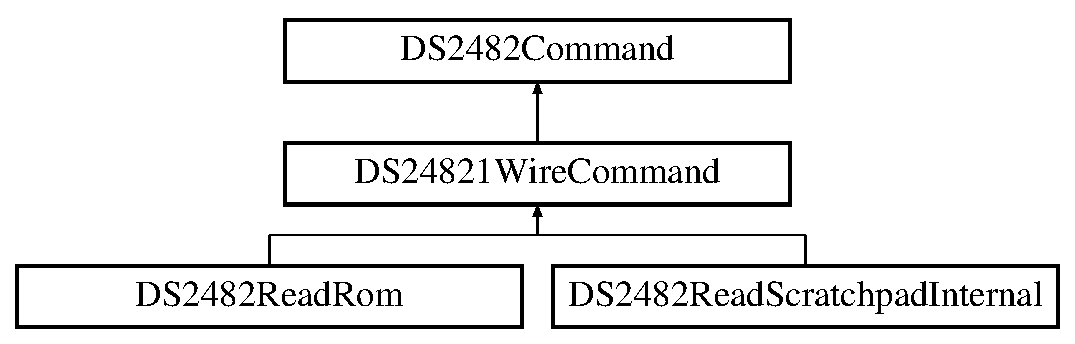
\includegraphics[height=3.000000cm]{class_d_s24821_wire_command}
\end{center}
\end{figure}
\subsection*{Public Member Functions}
\begin{DoxyCompactItemize}
\item 
\mbox{\Hypertarget{class_d_s24821_wire_command_a27e758f6a1de1f23ece963df35531dc5}\label{class_d_s24821_wire_command_a27e758f6a1de1f23ece963df35531dc5}} 
size\+\_\+t \mbox{\hyperlink{class_d_s24821_wire_command_a27e758f6a1de1f23ece963df35531dc5}{get\+Size}} () const
\begin{DoxyCompactList}\small\item\em Get the number of bytes that have been saved in the buffer so far. \end{DoxyCompactList}\item 
\mbox{\Hypertarget{class_d_s24821_wire_command_a71e935efbfc8c77e45cd45358fa3396c}\label{class_d_s24821_wire_command_a71e935efbfc8c77e45cd45358fa3396c}} 
const uint8\+\_\+t $\ast$ \mbox{\hyperlink{class_d_s24821_wire_command_a71e935efbfc8c77e45cd45358fa3396c}{get\+Buffer}} () const
\begin{DoxyCompactList}\small\item\em Gets a pointer to the buffer. \end{DoxyCompactList}\item 
\mbox{\hyperlink{class_d_s24821_wire_address}{D\+S24821\+Wire\+Address}} \mbox{\hyperlink{class_d_s24821_wire_command_ab00d3a0b120d3cc33675165d1174aa16}{get\+Address}} () const
\begin{DoxyCompactList}\small\item\em Gets the buffer as a 1-\/wire address. \end{DoxyCompactList}\item 
bool \mbox{\hyperlink{class_d_s24821_wire_command_a721ceae3f65419340b0ea0efa75a37a6}{check\+C\+RC}} () const
\begin{DoxyCompactList}\small\item\em Checks the C\+RC of the buffer. \end{DoxyCompactList}\end{DoxyCompactItemize}
\subsection*{Protected Member Functions}
\begin{DoxyCompactItemize}
\item 
\mbox{\Hypertarget{class_d_s24821_wire_command_a0c487fb5b756a58a9daa78ebc83bed6b}\label{class_d_s24821_wire_command_a0c487fb5b756a58a9daa78ebc83bed6b}} 
\mbox{\hyperlink{class_d_s24821_wire_command_a0c487fb5b756a58a9daa78ebc83bed6b}{D\+S24821\+Wire\+Command}} (\mbox{\hyperlink{class_d_s2482}{D\+S2482}} \&\mbox{\hyperlink{class_d_s2482_command_a54a41fb8a610ef2077f5e5377771aaf3}{parent}}, uint8\+\_\+t cmd, size\+\_\+t read\+Size, std\+::function$<$ void(\mbox{\hyperlink{class_d_s24821_wire_command}{D\+S24821\+Wire\+Command}} \&, int status)$>$ completion)
\begin{DoxyCompactList}\small\item\em Sends a 1-\/wire command and reads bytes back. Used internally. \end{DoxyCompactList}\item 
\mbox{\Hypertarget{class_d_s24821_wire_command_aa64fcd820dfc1621af7eeef0c03844c6}\label{class_d_s24821_wire_command_aa64fcd820dfc1621af7eeef0c03844c6}} 
virtual \mbox{\hyperlink{class_d_s24821_wire_command_aa64fcd820dfc1621af7eeef0c03844c6}{$\sim$\+D\+S24821\+Wire\+Command}} ()
\begin{DoxyCompactList}\small\item\em Destructor. \end{DoxyCompactList}\item 
\mbox{\Hypertarget{class_d_s24821_wire_command_ab07546a36f9d4e04f098e6aec81b0496}\label{class_d_s24821_wire_command_ab07546a36f9d4e04f098e6aec81b0496}} 
virtual int \mbox{\hyperlink{class_d_s24821_wire_command_ab07546a36f9d4e04f098e6aec81b0496}{loop}} ()
\begin{DoxyCompactList}\small\item\em Used to provide allow the command to executed. \end{DoxyCompactList}\end{DoxyCompactItemize}
\subsection*{Friends}
\begin{DoxyCompactItemize}
\item 
\mbox{\Hypertarget{class_d_s24821_wire_command_afeaf69274324e8dbeebede05c02d9c18}\label{class_d_s24821_wire_command_afeaf69274324e8dbeebede05c02d9c18}} 
class {\bfseries D\+S2482}
\end{DoxyCompactItemize}
\subsection*{Additional Inherited Members}


\subsection{Detailed Description}
Low-\/level class to send a 1-\/wire command and read a number of bytes back. You won\textquotesingle{}t need to call this directly. 

There is no run method in this class as it\textquotesingle{}s only subclassed by specific commands. 

\subsection{Member Function Documentation}
\mbox{\Hypertarget{class_d_s24821_wire_command_a721ceae3f65419340b0ea0efa75a37a6}\label{class_d_s24821_wire_command_a721ceae3f65419340b0ea0efa75a37a6}} 
\index{D\+S24821\+Wire\+Command@{D\+S24821\+Wire\+Command}!check\+C\+RC@{check\+C\+RC}}
\index{check\+C\+RC@{check\+C\+RC}!D\+S24821\+Wire\+Command@{D\+S24821\+Wire\+Command}}
\subsubsection{\texorpdfstring{check\+C\+R\+C()}{checkCRC()}}
{\footnotesize\ttfamily bool D\+S24821\+Wire\+Command\+::check\+C\+RC (\begin{DoxyParamCaption}{ }\end{DoxyParamCaption}) const}



Checks the C\+RC of the buffer. 

The assumption is that the C\+RC value will be at (offset -\/ 1). It will calculate the C\+RC of the bytes from 0 to (offset -\/ 2) inclusive. \mbox{\Hypertarget{class_d_s24821_wire_command_ab00d3a0b120d3cc33675165d1174aa16}\label{class_d_s24821_wire_command_ab00d3a0b120d3cc33675165d1174aa16}} 
\index{D\+S24821\+Wire\+Command@{D\+S24821\+Wire\+Command}!get\+Address@{get\+Address}}
\index{get\+Address@{get\+Address}!D\+S24821\+Wire\+Command@{D\+S24821\+Wire\+Command}}
\subsubsection{\texorpdfstring{get\+Address()}{getAddress()}}
{\footnotesize\ttfamily \mbox{\hyperlink{class_d_s24821_wire_address}{D\+S24821\+Wire\+Address}} D\+S24821\+Wire\+Command\+::get\+Address (\begin{DoxyParamCaption}{ }\end{DoxyParamCaption}) const}



Gets the buffer as a 1-\/wire address. 

A copy is returned as a \mbox{\hyperlink{class_d_s24821_wire_address}{D\+S24821\+Wire\+Address}} object. 

The documentation for this class was generated from the following files\+:\begin{DoxyCompactItemize}
\item 
src/D\+S2482-\/\+R\+K.\+h\item 
src/D\+S2482-\/\+R\+K.\+cpp\end{DoxyCompactItemize}

\hypertarget{class_d_s24821_wire_read_byte}{}\section{D\+S24821\+Wire\+Read\+Byte Class Reference}
\label{class_d_s24821_wire_read_byte}\index{D\+S24821\+Wire\+Read\+Byte@{D\+S24821\+Wire\+Read\+Byte}}


Low-\/level class to read a byte from the 1-\/wire bus.  




{\ttfamily \#include $<$D\+S2482-\/\+R\+K.\+h$>$}

Inheritance diagram for D\+S24821\+Wire\+Read\+Byte\+:\begin{figure}[H]
\begin{center}
\leavevmode
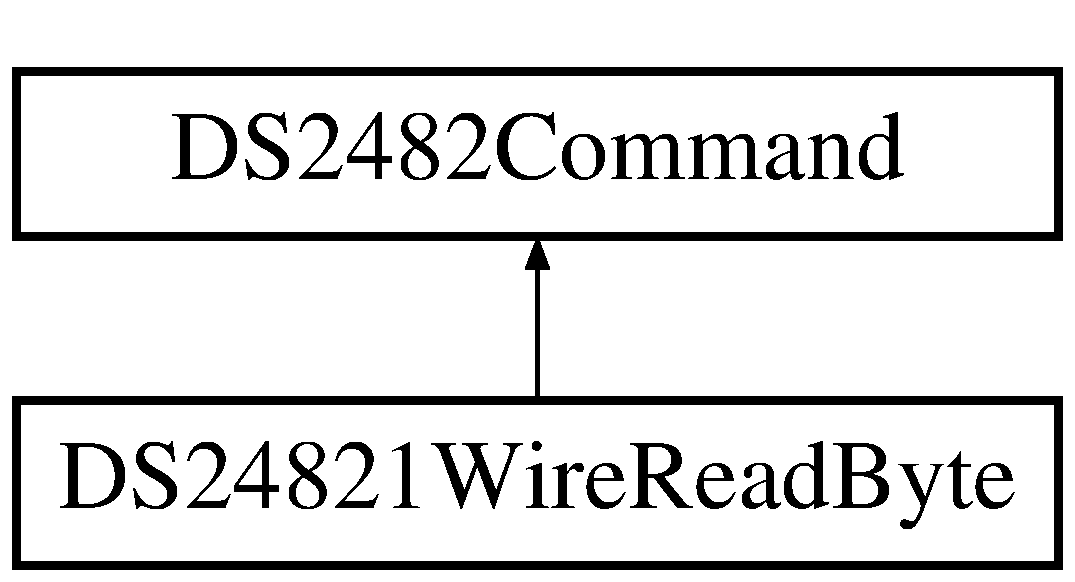
\includegraphics[height=2.000000cm]{class_d_s24821_wire_read_byte}
\end{center}
\end{figure}
\subsection*{Public Member Functions}
\begin{DoxyCompactItemize}
\item 
\mbox{\Hypertarget{class_d_s24821_wire_read_byte_a958288a6d8d3e7c970e668099dce3b82}\label{class_d_s24821_wire_read_byte_a958288a6d8d3e7c970e668099dce3b82}} 
uint8\+\_\+t \mbox{\hyperlink{class_d_s24821_wire_read_byte_a958288a6d8d3e7c970e668099dce3b82}{get\+Value}} () const
\begin{DoxyCompactList}\small\item\em Get the value that was read. Also is included as a parameter to the callback. \end{DoxyCompactList}\end{DoxyCompactItemize}
\subsection*{Static Public Member Functions}
\begin{DoxyCompactItemize}
\item 
\mbox{\Hypertarget{class_d_s24821_wire_read_byte_aa7e399c9eca3042d9d3002cd53516d42}\label{class_d_s24821_wire_read_byte_aa7e399c9eca3042d9d3002cd53516d42}} 
static \mbox{\hyperlink{class_d_s24821_wire_read_byte}{D\+S24821\+Wire\+Read\+Byte}} \& \mbox{\hyperlink{class_d_s24821_wire_read_byte_aa7e399c9eca3042d9d3002cd53516d42}{run}} (\mbox{\hyperlink{class_d_s2482}{D\+S2482}} \&\mbox{\hyperlink{class_d_s2482_command_a54a41fb8a610ef2077f5e5377771aaf3}{parent}}, std\+::function$<$ void(\mbox{\hyperlink{class_d_s24821_wire_read_byte}{D\+S24821\+Wire\+Read\+Byte}} \&, int, uint8\+\_\+t)$>$ completion)
\begin{DoxyCompactList}\small\item\em Low-\/level call to read a byte from the 1-\/wire bus. \end{DoxyCompactList}\end{DoxyCompactItemize}
\subsection*{Friends}
\begin{DoxyCompactItemize}
\item 
\mbox{\Hypertarget{class_d_s24821_wire_read_byte_afeaf69274324e8dbeebede05c02d9c18}\label{class_d_s24821_wire_read_byte_afeaf69274324e8dbeebede05c02d9c18}} 
class {\bfseries D\+S2482}
\end{DoxyCompactItemize}
\subsection*{Additional Inherited Members}


\subsection{Detailed Description}
Low-\/level class to read a byte from the 1-\/wire bus. 

You will likely use the higher-\/level functions instead.

As with all command objects, you do not typically construct one of these objects. Instead, use the static run method to handle allocating, initializing, and queueing the command. 

The documentation for this class was generated from the following files\+:\begin{DoxyCompactItemize}
\item 
src/D\+S2482-\/\+R\+K.\+h\item 
src/D\+S2482-\/\+R\+K.\+cpp\end{DoxyCompactItemize}

\hypertarget{class_d_s24821_wire_reset}{}\section{D\+S24821\+Wire\+Reset Class Reference}
\label{class_d_s24821_wire_reset}\index{D\+S24821\+Wire\+Reset@{D\+S24821\+Wire\+Reset}}


Resets the 1-\/wire bus.  




{\ttfamily \#include $<$D\+S2482-\/\+R\+K.\+h$>$}

Inheritance diagram for D\+S24821\+Wire\+Reset\+:\begin{figure}[H]
\begin{center}
\leavevmode
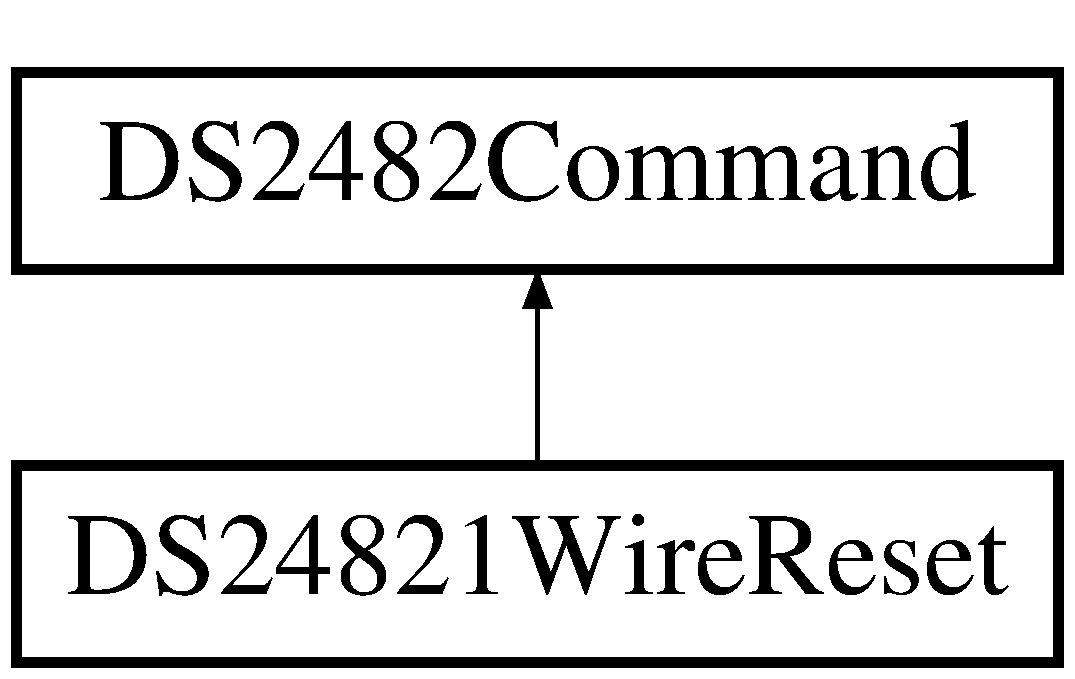
\includegraphics[height=2.000000cm]{class_d_s24821_wire_reset}
\end{center}
\end{figure}
\subsection*{Public Member Functions}
\begin{DoxyCompactItemize}
\item 
\mbox{\Hypertarget{class_d_s24821_wire_reset_a79cb9f726fce17b4ff23a4df739ede3b}\label{class_d_s24821_wire_reset_a79cb9f726fce17b4ff23a4df739ede3b}} 
bool \mbox{\hyperlink{class_d_s24821_wire_reset_a79cb9f726fce17b4ff23a4df739ede3b}{get\+Presence\+Detected}} () const
\begin{DoxyCompactList}\small\item\em Get whether a presence pulse was detected after 1-\/wire reset. Also passed to the completion function. \end{DoxyCompactList}\end{DoxyCompactItemize}
\subsection*{Static Public Member Functions}
\begin{DoxyCompactItemize}
\item 
\mbox{\Hypertarget{class_d_s24821_wire_reset_a39a32211363709147a294fb61a323034}\label{class_d_s24821_wire_reset_a39a32211363709147a294fb61a323034}} 
static \mbox{\hyperlink{class_d_s24821_wire_reset}{D\+S24821\+Wire\+Reset}} \& \mbox{\hyperlink{class_d_s24821_wire_reset_a39a32211363709147a294fb61a323034}{run}} (\mbox{\hyperlink{class_d_s2482}{D\+S2482}} \&\mbox{\hyperlink{class_d_s2482_command_a54a41fb8a610ef2077f5e5377771aaf3}{parent}}, std\+::function$<$ void(\mbox{\hyperlink{class_d_s24821_wire_reset}{D\+S24821\+Wire\+Reset}} \&, int status, bool presence\+Detected)$>$ completion)
\begin{DoxyCompactList}\small\item\em Low-\/level call to reset the 1-\/wire bus. \end{DoxyCompactList}\end{DoxyCompactItemize}
\subsection*{Friends}
\begin{DoxyCompactItemize}
\item 
\mbox{\Hypertarget{class_d_s24821_wire_reset_afeaf69274324e8dbeebede05c02d9c18}\label{class_d_s24821_wire_reset_afeaf69274324e8dbeebede05c02d9c18}} 
class {\bfseries D\+S2482}
\end{DoxyCompactItemize}
\subsection*{Additional Inherited Members}


\subsection{Detailed Description}
Resets the 1-\/wire bus. 

You normally don\textquotesingle{}t need to do this yourself, as it\textquotesingle{}s done internally when necessary, such as before a bus search.

As with all command objects, you do not typically construct one of these objects. Instead, use the static run method to handle allocating, initializing, and queueing the command. 

The documentation for this class was generated from the following files\+:\begin{DoxyCompactItemize}
\item 
src/D\+S2482-\/\+R\+K.\+h\item 
src/D\+S2482-\/\+R\+K.\+cpp\end{DoxyCompactItemize}

\hypertarget{class_d_s24821_wire_send_address}{}\section{D\+S24821\+Wire\+Send\+Address Class Reference}
\label{class_d_s24821_wire_send_address}\index{D\+S24821\+Wire\+Send\+Address@{D\+S24821\+Wire\+Send\+Address}}


Low-\/level class to send a 1-\/wire address. You won\textquotesingle{}t need to call this directly.  




{\ttfamily \#include $<$D\+S2482-\/\+R\+K.\+h$>$}

Inheritance diagram for D\+S24821\+Wire\+Send\+Address\+:\begin{figure}[H]
\begin{center}
\leavevmode
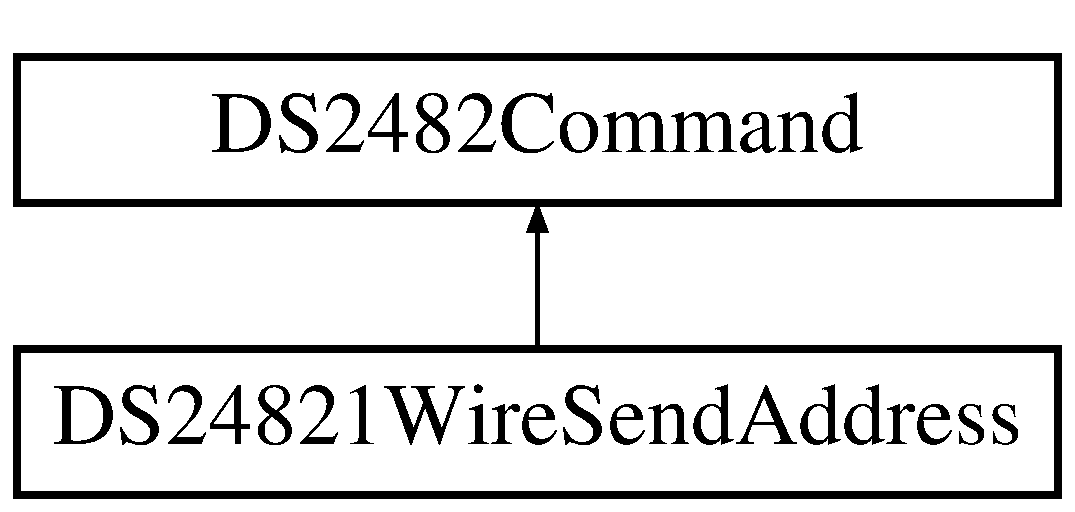
\includegraphics[height=2.000000cm]{class_d_s24821_wire_send_address}
\end{center}
\end{figure}
\subsection*{Static Public Member Functions}
\begin{DoxyCompactItemize}
\item 
\mbox{\Hypertarget{class_d_s24821_wire_send_address_a6ca16b182b5935d64d400b1bd7f35adf}\label{class_d_s24821_wire_send_address_a6ca16b182b5935d64d400b1bd7f35adf}} 
static \mbox{\hyperlink{class_d_s24821_wire_send_address}{D\+S24821\+Wire\+Send\+Address}} \& \mbox{\hyperlink{class_d_s24821_wire_send_address_a6ca16b182b5935d64d400b1bd7f35adf}{run}} (\mbox{\hyperlink{class_d_s2482}{D\+S2482}} \&\mbox{\hyperlink{class_d_s2482_command_a54a41fb8a610ef2077f5e5377771aaf3}{parent}}, const \mbox{\hyperlink{class_d_s24821_wire_address}{D\+S24821\+Wire\+Address}} \&addr, std\+::function$<$ void(\mbox{\hyperlink{class_d_s24821_wire_send_address}{D\+S24821\+Wire\+Send\+Address}} \&, int status)$>$ completion)
\begin{DoxyCompactList}\small\item\em Runs a 1-\/wire send address to send an address over the wire -\/ used internally. \end{DoxyCompactList}\end{DoxyCompactItemize}
\subsection*{Friends}
\begin{DoxyCompactItemize}
\item 
\mbox{\Hypertarget{class_d_s24821_wire_send_address_afeaf69274324e8dbeebede05c02d9c18}\label{class_d_s24821_wire_send_address_afeaf69274324e8dbeebede05c02d9c18}} 
class {\bfseries D\+S2482}
\end{DoxyCompactItemize}
\subsection*{Additional Inherited Members}


\subsection{Detailed Description}
Low-\/level class to send a 1-\/wire address. You won\textquotesingle{}t need to call this directly. 

This is used after sending a M\+A\+T\+C\+H\+\_\+\+R\+OM to send the actual R\+OM address to match.

As with all command objects, you do not typically construct one of these objects. Instead, use the static run method to handle allocating, initializing, and queueing the command. 

The documentation for this class was generated from the following files\+:\begin{DoxyCompactItemize}
\item 
src/D\+S2482-\/\+R\+K.\+h\item 
src/D\+S2482-\/\+R\+K.\+cpp\end{DoxyCompactItemize}

\hypertarget{class_d_s24821_wire_triplet}{}\section{D\+S24821\+Wire\+Triplet Class Reference}
\label{class_d_s24821_wire_triplet}\index{D\+S24821\+Wire\+Triplet@{D\+S24821\+Wire\+Triplet}}


Low-\/level class to generate a 1-\/wire triplet, used for bus search. You won\textquotesingle{}t need to call this directly.  




{\ttfamily \#include $<$D\+S2482-\/\+R\+K.\+h$>$}

Inheritance diagram for D\+S24821\+Wire\+Triplet\+:\begin{figure}[H]
\begin{center}
\leavevmode
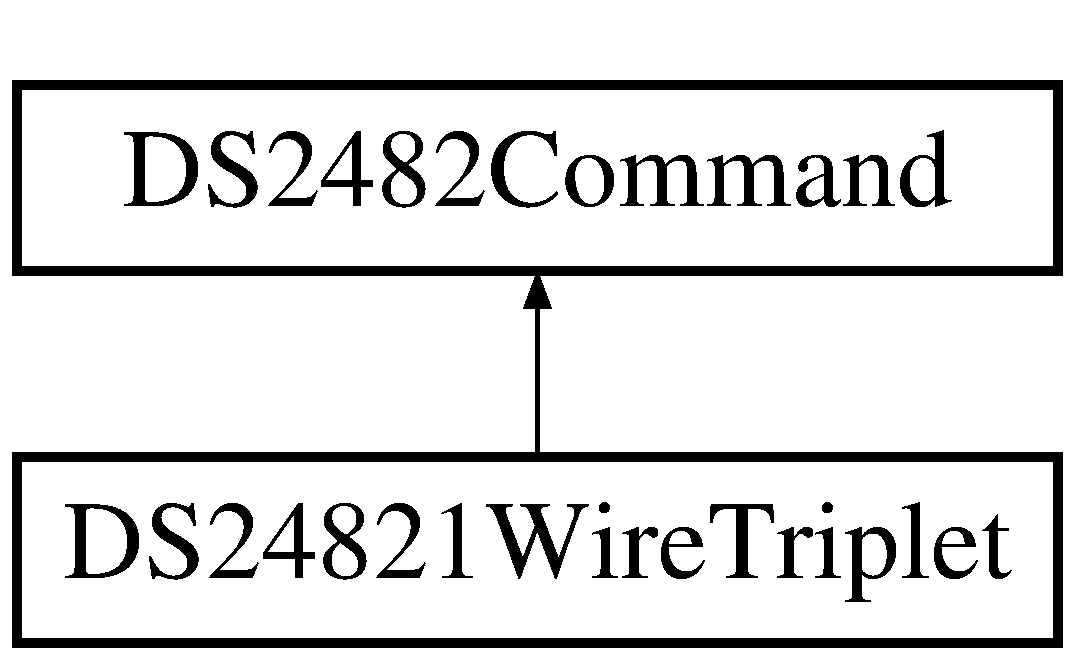
\includegraphics[height=2.000000cm]{class_d_s24821_wire_triplet}
\end{center}
\end{figure}
\subsection*{Public Member Functions}
\begin{DoxyCompactItemize}
\item 
\mbox{\Hypertarget{class_d_s24821_wire_triplet_add828cd5c41a8052bd1f004167f45856}\label{class_d_s24821_wire_triplet_add828cd5c41a8052bd1f004167f45856}} 
uint8\+\_\+t \mbox{\hyperlink{class_d_s24821_wire_triplet_add828cd5c41a8052bd1f004167f45856}{get\+Status\+Bits}} () const
\begin{DoxyCompactList}\small\item\em Gets the status bit result from 1-\/wire triplet. \end{DoxyCompactList}\item 
\mbox{\Hypertarget{class_d_s24821_wire_triplet_a904b22b4d426bc6eab5e29812f62d326}\label{class_d_s24821_wire_triplet_a904b22b4d426bc6eab5e29812f62d326}} 
bool \mbox{\hyperlink{class_d_s24821_wire_triplet_a904b22b4d426bc6eab5e29812f62d326}{get\+S\+BR}} () const
\begin{DoxyCompactList}\small\item\em Returns the state of the S\+BR in the status register. \end{DoxyCompactList}\item 
\mbox{\Hypertarget{class_d_s24821_wire_triplet_a564c45067d9502575ebcad4d7f0fe59b}\label{class_d_s24821_wire_triplet_a564c45067d9502575ebcad4d7f0fe59b}} 
bool \mbox{\hyperlink{class_d_s24821_wire_triplet_a564c45067d9502575ebcad4d7f0fe59b}{get\+T\+SB}} () const
\begin{DoxyCompactList}\small\item\em Returns the state of the T\+SB in the status register. \end{DoxyCompactList}\item 
\mbox{\Hypertarget{class_d_s24821_wire_triplet_afa065b80fd93597f05b2008b791e0325}\label{class_d_s24821_wire_triplet_afa065b80fd93597f05b2008b791e0325}} 
bool \mbox{\hyperlink{class_d_s24821_wire_triplet_afa065b80fd93597f05b2008b791e0325}{get\+D\+IR}} () const
\begin{DoxyCompactList}\small\item\em Returns the state of the D\+IR in the status register. \end{DoxyCompactList}\end{DoxyCompactItemize}
\subsection*{Static Public Member Functions}
\begin{DoxyCompactItemize}
\item 
\mbox{\Hypertarget{class_d_s24821_wire_triplet_ab6f4e38254420ee2aca30bbc7cb44213}\label{class_d_s24821_wire_triplet_ab6f4e38254420ee2aca30bbc7cb44213}} 
static \mbox{\hyperlink{class_d_s24821_wire_triplet}{D\+S24821\+Wire\+Triplet}} \& \mbox{\hyperlink{class_d_s24821_wire_triplet_ab6f4e38254420ee2aca30bbc7cb44213}{run}} (\mbox{\hyperlink{class_d_s2482}{D\+S2482}} \&\mbox{\hyperlink{class_d_s2482_command_a54a41fb8a610ef2077f5e5377771aaf3}{parent}}, bool dir\+In, std\+::function$<$ void(\mbox{\hyperlink{class_d_s24821_wire_triplet}{D\+S24821\+Wire\+Triplet}} \&, int status)$>$ completion)
\begin{DoxyCompactList}\small\item\em Runs a 1-\/wire triplet operation -\/ used internally to do bus search. \end{DoxyCompactList}\end{DoxyCompactItemize}
\subsection*{Friends}
\begin{DoxyCompactItemize}
\item 
\mbox{\Hypertarget{class_d_s24821_wire_triplet_afeaf69274324e8dbeebede05c02d9c18}\label{class_d_s24821_wire_triplet_afeaf69274324e8dbeebede05c02d9c18}} 
class {\bfseries D\+S2482}
\end{DoxyCompactItemize}
\subsection*{Additional Inherited Members}


\subsection{Detailed Description}
Low-\/level class to generate a 1-\/wire triplet, used for bus search. You won\textquotesingle{}t need to call this directly. 

As with all command objects, you do not typically construct one of these objects. Instead, use the static run method to handle allocating, initializing, and queueing the command. 

The documentation for this class was generated from the following files\+:\begin{DoxyCompactItemize}
\item 
src/D\+S2482-\/\+R\+K.\+h\item 
src/D\+S2482-\/\+R\+K.\+cpp\end{DoxyCompactItemize}

\hypertarget{class_d_s24821_wire_write_byte}{}\section{D\+S24821\+Wire\+Write\+Byte Class Reference}
\label{class_d_s24821_wire_write_byte}\index{D\+S24821\+Wire\+Write\+Byte@{D\+S24821\+Wire\+Write\+Byte}}


Low-\/level class to write a byte to the 1-\/wire bus.  




{\ttfamily \#include $<$D\+S2482-\/\+R\+K.\+h$>$}

Inheritance diagram for D\+S24821\+Wire\+Write\+Byte\+:\begin{figure}[H]
\begin{center}
\leavevmode
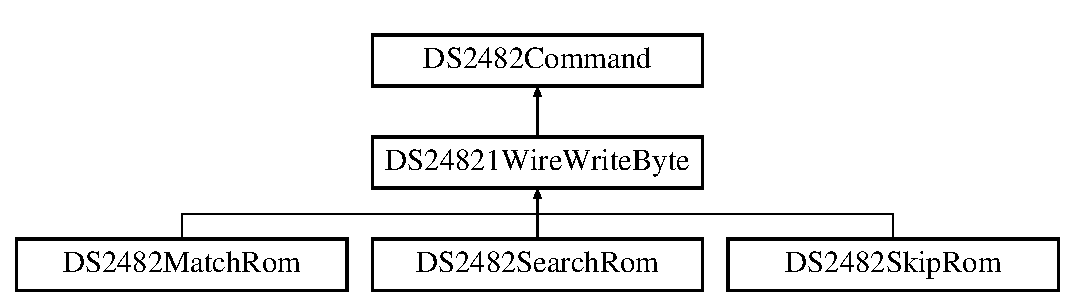
\includegraphics[height=3.000000cm]{class_d_s24821_wire_write_byte}
\end{center}
\end{figure}
\subsection*{Static Public Member Functions}
\begin{DoxyCompactItemize}
\item 
\mbox{\Hypertarget{class_d_s24821_wire_write_byte_a2398d9539b7038f70e277b204f4e8ead}\label{class_d_s24821_wire_write_byte_a2398d9539b7038f70e277b204f4e8ead}} 
static \mbox{\hyperlink{class_d_s24821_wire_write_byte}{D\+S24821\+Wire\+Write\+Byte}} \& \mbox{\hyperlink{class_d_s24821_wire_write_byte_a2398d9539b7038f70e277b204f4e8ead}{run}} (\mbox{\hyperlink{class_d_s2482}{D\+S2482}} \&\mbox{\hyperlink{class_d_s2482_command_a54a41fb8a610ef2077f5e5377771aaf3}{parent}}, uint8\+\_\+t value, std\+::function$<$ void(\mbox{\hyperlink{class_d_s24821_wire_write_byte}{D\+S24821\+Wire\+Write\+Byte}} \&, int status)$>$ completion)
\begin{DoxyCompactList}\small\item\em Low-\/level call to write a byte to the 1-\/wire bus. \end{DoxyCompactList}\end{DoxyCompactItemize}
\subsection*{Protected Member Functions}
\begin{DoxyCompactItemize}
\item 
\mbox{\Hypertarget{class_d_s24821_wire_write_byte_ac4662898e8aaf037272157d9eed86434}\label{class_d_s24821_wire_write_byte_ac4662898e8aaf037272157d9eed86434}} 
\mbox{\hyperlink{class_d_s24821_wire_write_byte_ac4662898e8aaf037272157d9eed86434}{D\+S24821\+Wire\+Write\+Byte}} (\mbox{\hyperlink{class_d_s2482}{D\+S2482}} \&\mbox{\hyperlink{class_d_s2482_command_a54a41fb8a610ef2077f5e5377771aaf3}{parent}}, uint8\+\_\+t value, std\+::function$<$ void(\mbox{\hyperlink{class_d_s24821_wire_write_byte}{D\+S24821\+Wire\+Write\+Byte}} \&, int)$>$ completion)
\begin{DoxyCompactList}\small\item\em Used internally -\/ you won\textquotesingle{}t use this directly, but it is used by \mbox{\hyperlink{class_d_s2482_read_rom}{D\+S2482\+Read\+Rom}}, \mbox{\hyperlink{class_d_s2482_search_rom}{D\+S2482\+Search\+Rom}}, etc. \end{DoxyCompactList}\item 
\mbox{\Hypertarget{class_d_s24821_wire_write_byte_a5a23b89bb74a638af353ef44bf75ce37}\label{class_d_s24821_wire_write_byte_a5a23b89bb74a638af353ef44bf75ce37}} 
virtual int \mbox{\hyperlink{class_d_s24821_wire_write_byte_a5a23b89bb74a638af353ef44bf75ce37}{loop}} ()
\begin{DoxyCompactList}\small\item\em Overridden by subclasses to do things; typically to run the state machine. \end{DoxyCompactList}\end{DoxyCompactItemize}
\subsection*{Friends}
\begin{DoxyCompactItemize}
\item 
\mbox{\Hypertarget{class_d_s24821_wire_write_byte_afeaf69274324e8dbeebede05c02d9c18}\label{class_d_s24821_wire_write_byte_afeaf69274324e8dbeebede05c02d9c18}} 
class {\bfseries D\+S2482}
\end{DoxyCompactItemize}
\subsection*{Additional Inherited Members}


\subsection{Detailed Description}
Low-\/level class to write a byte to the 1-\/wire bus. 

You will likely use the higher-\/level functions instead.

As with all command objects, you do not typically construct one of these objects. Instead, use the static run method to handle allocating, initializing, and queueing the command. 

The documentation for this class was generated from the following files\+:\begin{DoxyCompactItemize}
\item 
src/D\+S2482-\/\+R\+K.\+h\item 
src/D\+S2482-\/\+R\+K.\+cpp\end{DoxyCompactItemize}

\hypertarget{class_d_s2482_channel_select}{}\section{D\+S2482\+Channel\+Select Class Reference}
\label{class_d_s2482_channel_select}\index{D\+S2482\+Channel\+Select@{D\+S2482\+Channel\+Select}}


When using the D\+S2482-\/800, this selects which of the 8 channels you want to work with.  




{\ttfamily \#include $<$D\+S2482-\/\+R\+K.\+h$>$}

Inheritance diagram for D\+S2482\+Channel\+Select\+:\begin{figure}[H]
\begin{center}
\leavevmode
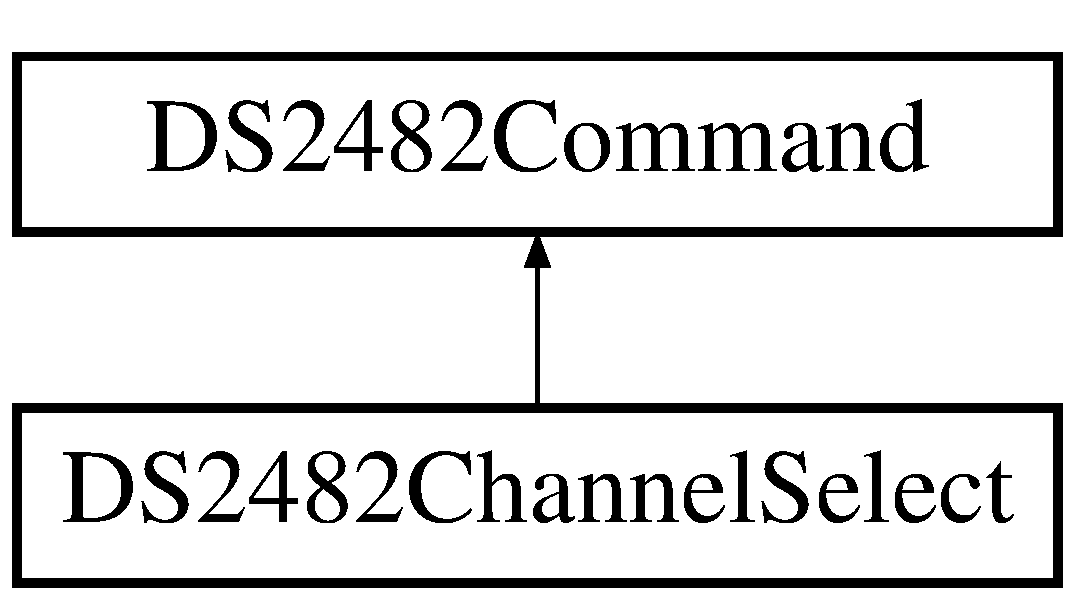
\includegraphics[height=2.000000cm]{class_d_s2482_channel_select}
\end{center}
\end{figure}
\subsection*{Static Public Member Functions}
\begin{DoxyCompactItemize}
\item 
static \mbox{\hyperlink{class_d_s2482_channel_select}{D\+S2482\+Channel\+Select}} \& \mbox{\hyperlink{class_d_s2482_channel_select_a32cd9d686395cf5425790e9518664740}{run}} (\mbox{\hyperlink{class_d_s2482}{D\+S2482}} \&\mbox{\hyperlink{class_d_s2482_command_a54a41fb8a610ef2077f5e5377771aaf3}{parent}}, int channel, std\+::function$<$ void(\mbox{\hyperlink{class_d_s2482_channel_select}{D\+S2482\+Channel\+Select}} \&, int status)$>$ completion)
\begin{DoxyCompactList}\small\item\em When using the D\+S2482-\/800, this selects which of the 8 channels you want to work with. \end{DoxyCompactList}\end{DoxyCompactItemize}
\subsection*{Friends}
\begin{DoxyCompactItemize}
\item 
\mbox{\Hypertarget{class_d_s2482_channel_select_afeaf69274324e8dbeebede05c02d9c18}\label{class_d_s2482_channel_select_afeaf69274324e8dbeebede05c02d9c18}} 
class {\bfseries D\+S2482}
\end{DoxyCompactItemize}
\subsection*{Additional Inherited Members}


\subsection{Detailed Description}
When using the D\+S2482-\/800, this selects which of the 8 channels you want to work with. 

On power-\/up, channel 0 is selected. Valid channel numbers are 0 $<$= channel $<$ 8.

As with all command objects, you do not typically construct one of these objects. Instead, use the static run method to handle allocating, initializing, and queueing the command. 

\subsection{Member Function Documentation}
\mbox{\Hypertarget{class_d_s2482_channel_select_a32cd9d686395cf5425790e9518664740}\label{class_d_s2482_channel_select_a32cd9d686395cf5425790e9518664740}} 
\index{D\+S2482\+Channel\+Select@{D\+S2482\+Channel\+Select}!run@{run}}
\index{run@{run}!D\+S2482\+Channel\+Select@{D\+S2482\+Channel\+Select}}
\subsubsection{\texorpdfstring{run()}{run()}}
{\footnotesize\ttfamily \mbox{\hyperlink{class_d_s2482_channel_select}{D\+S2482\+Channel\+Select}} \& D\+S2482\+Channel\+Select\+::run (\begin{DoxyParamCaption}\item[{\mbox{\hyperlink{class_d_s2482}{D\+S2482}} \&}]{parent,  }\item[{int}]{channel,  }\item[{std\+::function$<$ void(\mbox{\hyperlink{class_d_s2482_channel_select}{D\+S2482\+Channel\+Select}} \&, int status)$>$}]{completion }\end{DoxyParamCaption})\hspace{0.3cm}{\ttfamily [static]}}



When using the D\+S2482-\/800, this selects which of the 8 channels you want to work with. 


\begin{DoxyParams}{Parameters}
{\em parent} & The D\+S2482-\/800 you want to send the command to.\\
\hline
{\em channel} & The channel number to set to where 0 $<$= channel $<$ 8. Default at power-\/up is 0.\\
\hline
{\em completion} & The completion handler lambda function. status is the result status of the call; if \mbox{\hyperlink{class_d_s2482_command_a8ffcf84807c97928dbfc61d75788e32b}{D\+S2482\+Command\+::\+R\+E\+S\+U\+L\+T\+\_\+\+D\+O\+NE}} then the call succeeded.\\
\hline
\end{DoxyParams}
This call executes asynchronously. The completion function is called when complete or an error occurs. 

The documentation for this class was generated from the following files\+:\begin{DoxyCompactItemize}
\item 
src/D\+S2482-\/\+R\+K.\+h\item 
src/D\+S2482-\/\+R\+K.\+cpp\end{DoxyCompactItemize}

\hypertarget{class_d_s2482_check_bus_command}{}\section{D\+S2482\+Check\+Bus\+Command Class Reference}
\label{class_d_s2482_check_bus_command}\index{D\+S2482\+Check\+Bus\+Command@{D\+S2482\+Check\+Bus\+Command}}


Checks the 1-\/wire bus to determine if it\textquotesingle{}s single drop or multi-\/drop.  




{\ttfamily \#include $<$D\+S2482-\/\+R\+K.\+h$>$}

Inheritance diagram for D\+S2482\+Check\+Bus\+Command\+:\begin{figure}[H]
\begin{center}
\leavevmode
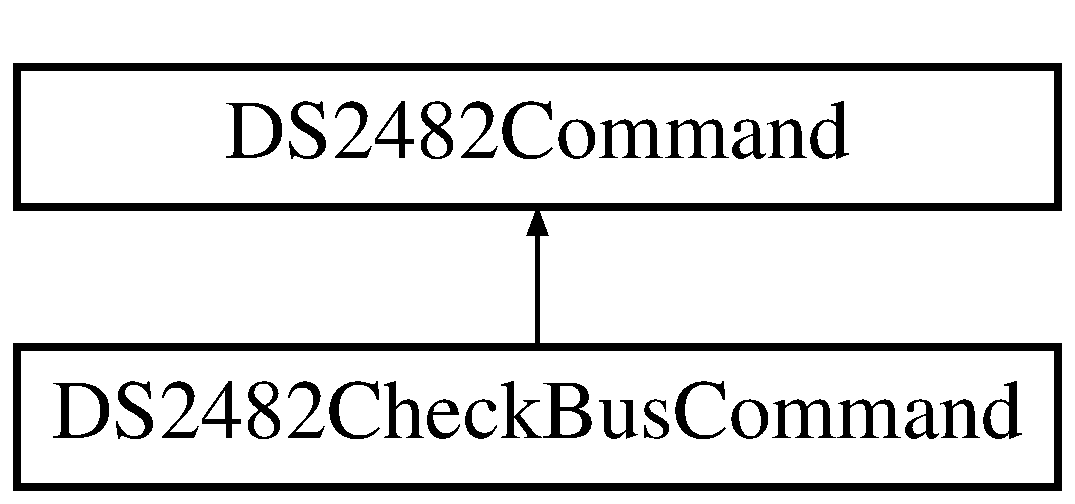
\includegraphics[height=2.000000cm]{class_d_s2482_check_bus_command}
\end{center}
\end{figure}
\subsection*{Public Member Functions}
\begin{DoxyCompactItemize}
\item 
int \mbox{\hyperlink{class_d_s2482_check_bus_command_a2d374709f24c8d7ad0c48766d7f072ee}{get\+Bus\+Status}} () const
\begin{DoxyCompactList}\small\item\em Gets the bus status\+: N\+O\+\_\+\+D\+E\+V\+I\+C\+ES, N\+O\+\_\+\+D\+E\+V\+I\+C\+ES, or M\+U\+L\+T\+I\+\_\+\+D\+R\+OP. \end{DoxyCompactList}\item 
const \mbox{\hyperlink{class_d_s24821_wire_address}{D\+S24821\+Wire\+Address}} \& \mbox{\hyperlink{class_d_s2482_check_bus_command_ac768c4e5d7bae840e451323cabc3c2de}{get\+Address}} () const
\begin{DoxyCompactList}\small\item\em If S\+I\+N\+G\+L\+E\+\_\+\+D\+R\+OP, gets the address of the single device on the bus. \end{DoxyCompactList}\end{DoxyCompactItemize}
\subsection*{Static Public Member Functions}
\begin{DoxyCompactItemize}
\item 
static \mbox{\hyperlink{class_d_s2482_check_bus_command}{D\+S2482\+Check\+Bus\+Command}} \& \mbox{\hyperlink{class_d_s2482_check_bus_command_a6710655a1ac2abc35d08db156d215c75}{run}} (\mbox{\hyperlink{class_d_s2482}{D\+S2482}} \&\mbox{\hyperlink{class_d_s2482_command_a54a41fb8a610ef2077f5e5377771aaf3}{parent}}, std\+::function$<$ void(\mbox{\hyperlink{class_d_s2482_check_bus_command}{D\+S2482\+Check\+Bus\+Command}} \&, int status, int bus\+Status)$>$ completion)
\begin{DoxyCompactList}\small\item\em Check the 1-\/wire bus to see if there are 0, 1, or more devices on it. \end{DoxyCompactList}\end{DoxyCompactItemize}
\subsection*{Static Public Attributes}
\begin{DoxyCompactItemize}
\item 
\mbox{\Hypertarget{class_d_s2482_check_bus_command_a926bd84843d75b022d88c896fd4608c1}\label{class_d_s2482_check_bus_command_a926bd84843d75b022d88c896fd4608c1}} 
static const int \mbox{\hyperlink{class_d_s2482_check_bus_command_a926bd84843d75b022d88c896fd4608c1}{N\+O\+\_\+\+D\+E\+V\+I\+C\+ES}} = 0
\begin{DoxyCompactList}\small\item\em There are 0 devices on the 1-\/wire bus. \end{DoxyCompactList}\item 
\mbox{\Hypertarget{class_d_s2482_check_bus_command_acf9addb2b671bfc9567dd58228379ec5}\label{class_d_s2482_check_bus_command_acf9addb2b671bfc9567dd58228379ec5}} 
static const int \mbox{\hyperlink{class_d_s2482_check_bus_command_acf9addb2b671bfc9567dd58228379ec5}{S\+I\+N\+G\+L\+E\+\_\+\+D\+R\+OP}} = 1
\begin{DoxyCompactList}\small\item\em There is 1 device on the 1-\/wire bus. An empty address can be used to identify the single device. \end{DoxyCompactList}\item 
\mbox{\Hypertarget{class_d_s2482_check_bus_command_af268c37a135b78ae684adfebeee349c1}\label{class_d_s2482_check_bus_command_af268c37a135b78ae684adfebeee349c1}} 
static const int \mbox{\hyperlink{class_d_s2482_check_bus_command_af268c37a135b78ae684adfebeee349c1}{M\+U\+L\+T\+I\+\_\+\+D\+R\+OP}} = 2
\begin{DoxyCompactList}\small\item\em There are 2 or more devices on the 1-\/wire bus. Addressing is required. \end{DoxyCompactList}\end{DoxyCompactItemize}
\subsection*{Friends}
\begin{DoxyCompactItemize}
\item 
\mbox{\Hypertarget{class_d_s2482_check_bus_command_afeaf69274324e8dbeebede05c02d9c18}\label{class_d_s2482_check_bus_command_afeaf69274324e8dbeebede05c02d9c18}} 
class {\bfseries D\+S2482}
\end{DoxyCompactItemize}
\subsection*{Additional Inherited Members}


\subsection{Detailed Description}
Checks the 1-\/wire bus to determine if it\textquotesingle{}s single drop or multi-\/drop. 

Completion is called with N\+O\+\_\+\+D\+E\+V\+I\+C\+ES, S\+I\+N\+G\+L\+E\+\_\+\+D\+R\+OP, or M\+U\+L\+T\+I\+\_\+\+D\+R\+OP indicating 0, 1, or more sensors on the 1-\/wire bus.

As with all command objects, you do not typically construct one of these objects. Instead, use the static run method to handle allocating, initializing, and queueing the command. 

\subsection{Member Function Documentation}
\mbox{\Hypertarget{class_d_s2482_check_bus_command_ac768c4e5d7bae840e451323cabc3c2de}\label{class_d_s2482_check_bus_command_ac768c4e5d7bae840e451323cabc3c2de}} 
\index{D\+S2482\+Check\+Bus\+Command@{D\+S2482\+Check\+Bus\+Command}!get\+Address@{get\+Address}}
\index{get\+Address@{get\+Address}!D\+S2482\+Check\+Bus\+Command@{D\+S2482\+Check\+Bus\+Command}}
\subsubsection{\texorpdfstring{get\+Address()}{getAddress()}}
{\footnotesize\ttfamily const \mbox{\hyperlink{class_d_s24821_wire_address}{D\+S24821\+Wire\+Address}}\& D\+S2482\+Check\+Bus\+Command\+::get\+Address (\begin{DoxyParamCaption}{ }\end{DoxyParamCaption}) const\hspace{0.3cm}{\ttfamily [inline]}}



If S\+I\+N\+G\+L\+E\+\_\+\+D\+R\+OP, gets the address of the single device on the bus. 

Note that for D\+S2482\+Get\+Temperature you don\textquotesingle{}t need the address for single drop; you can just pass an empty \mbox{\hyperlink{class_d_s24821_wire_address}{D\+S24821\+Wire\+Address}} and it will automatally use the only device on the bus. \mbox{\Hypertarget{class_d_s2482_check_bus_command_a2d374709f24c8d7ad0c48766d7f072ee}\label{class_d_s2482_check_bus_command_a2d374709f24c8d7ad0c48766d7f072ee}} 
\index{D\+S2482\+Check\+Bus\+Command@{D\+S2482\+Check\+Bus\+Command}!get\+Bus\+Status@{get\+Bus\+Status}}
\index{get\+Bus\+Status@{get\+Bus\+Status}!D\+S2482\+Check\+Bus\+Command@{D\+S2482\+Check\+Bus\+Command}}
\subsubsection{\texorpdfstring{get\+Bus\+Status()}{getBusStatus()}}
{\footnotesize\ttfamily int D\+S2482\+Check\+Bus\+Command\+::get\+Bus\+Status (\begin{DoxyParamCaption}{ }\end{DoxyParamCaption}) const\hspace{0.3cm}{\ttfamily [inline]}}



Gets the bus status\+: N\+O\+\_\+\+D\+E\+V\+I\+C\+ES, N\+O\+\_\+\+D\+E\+V\+I\+C\+ES, or M\+U\+L\+T\+I\+\_\+\+D\+R\+OP. 

You normally don\textquotesingle{}t need this because it\textquotesingle{}s passed as a parameter to the completion lambda. \mbox{\Hypertarget{class_d_s2482_check_bus_command_a6710655a1ac2abc35d08db156d215c75}\label{class_d_s2482_check_bus_command_a6710655a1ac2abc35d08db156d215c75}} 
\index{D\+S2482\+Check\+Bus\+Command@{D\+S2482\+Check\+Bus\+Command}!run@{run}}
\index{run@{run}!D\+S2482\+Check\+Bus\+Command@{D\+S2482\+Check\+Bus\+Command}}
\subsubsection{\texorpdfstring{run()}{run()}}
{\footnotesize\ttfamily \mbox{\hyperlink{class_d_s2482_check_bus_command}{D\+S2482\+Check\+Bus\+Command}} \& D\+S2482\+Check\+Bus\+Command\+::run (\begin{DoxyParamCaption}\item[{\mbox{\hyperlink{class_d_s2482}{D\+S2482}} \&}]{parent,  }\item[{std\+::function$<$ void(\mbox{\hyperlink{class_d_s2482_check_bus_command}{D\+S2482\+Check\+Bus\+Command}} \&, int status, int bus\+Status)$>$}]{completion }\end{DoxyParamCaption})\hspace{0.3cm}{\ttfamily [static]}}



Check the 1-\/wire bus to see if there are 0, 1, or more devices on it. 


\begin{DoxyParams}{Parameters}
{\em parent} & The \mbox{\hyperlink{class_d_s2482}{D\+S2482}} you want to send the command to. If it\textquotesingle{}s a D\+S2482\+\_\+800, make sure you set the channel as well.\\
\hline
{\em completion} & The completion handler lambda function. status is the result status of the call; if \mbox{\hyperlink{class_d_s2482_command_a8ffcf84807c97928dbfc61d75788e32b}{D\+S2482\+Command\+::\+R\+E\+S\+U\+L\+T\+\_\+\+D\+O\+NE}} then the call succeeded. If it\textquotesingle{}s any other value an error occurred. The bus\+Status is one of N\+O\+\_\+\+D\+E\+V\+I\+C\+ES, S\+I\+N\+G\+L\+E\+\_\+\+D\+R\+OP, or M\+U\+L\+T\+I\+\_\+\+D\+R\+OP indicating 0, 1, or more sensors on the 1-\/wire bus.\\
\hline
\end{DoxyParams}
This call executes asynchronously. The completion function is called when complete or an error occurs. 

The documentation for this class was generated from the following files\+:\begin{DoxyCompactItemize}
\item 
src/D\+S2482-\/\+R\+K.\+h\item 
src/D\+S2482-\/\+R\+K.\+cpp\end{DoxyCompactItemize}

\hypertarget{class_d_s2482_command}{}\section{D\+S2482\+Command Class Reference}
\label{class_d_s2482_command}\index{D\+S2482\+Command@{D\+S2482\+Command}}


Useful static constants, but the class is mostly just a base class for other commands.  




{\ttfamily \#include $<$D\+S2482-\/\+R\+K.\+h$>$}

Inheritance diagram for D\+S2482\+Command\+:\begin{figure}[H]
\begin{center}
\leavevmode
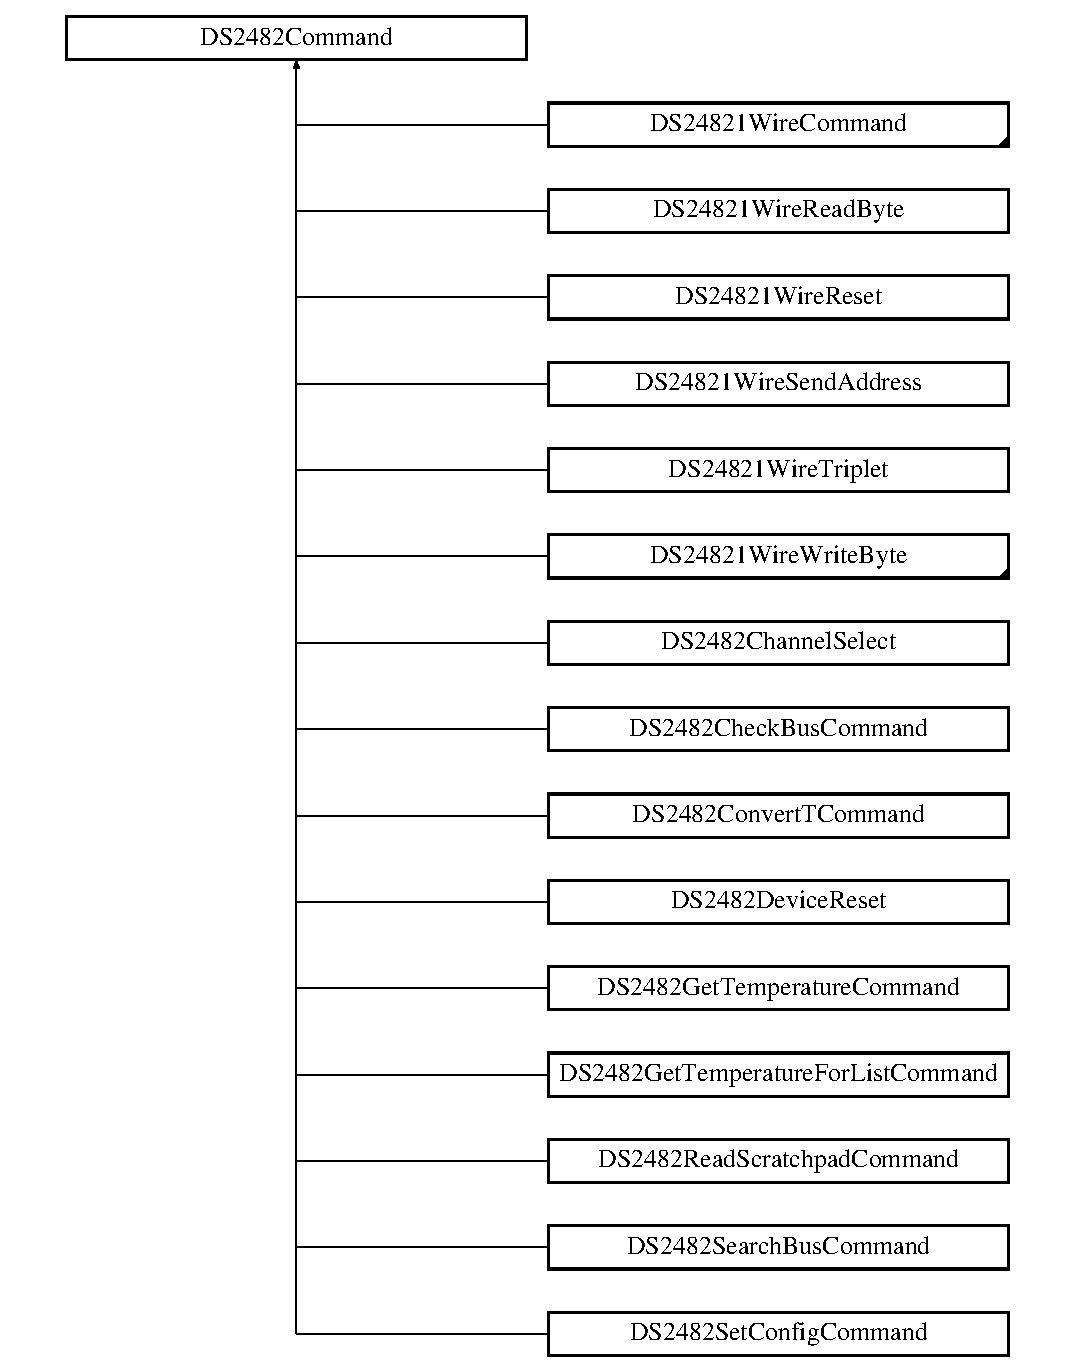
\includegraphics[height=12.000000cm]{class_d_s2482_command}
\end{center}
\end{figure}
\subsection*{Public Member Functions}
\begin{DoxyCompactItemize}
\item 
\mbox{\hyperlink{class_d_s2482_command_afafdd341bb8dbddf755a1ba2aaee79db}{D\+S2482\+Command}} (\mbox{\hyperlink{class_d_s2482}{D\+S2482}} \&\mbox{\hyperlink{class_d_s2482_command_a54a41fb8a610ef2077f5e5377771aaf3}{parent}})
\begin{DoxyCompactList}\small\item\em Construct a command object. \end{DoxyCompactList}\item 
\mbox{\Hypertarget{class_d_s2482_command_abc7ef041a3124b81183a9e37ab29b5bd}\label{class_d_s2482_command_abc7ef041a3124b81183a9e37ab29b5bd}} 
virtual \mbox{\hyperlink{class_d_s2482_command_abc7ef041a3124b81183a9e37ab29b5bd}{$\sim$\+D\+S2482\+Command}} ()
\begin{DoxyCompactList}\small\item\em Destructor. \end{DoxyCompactList}\item 
\mbox{\Hypertarget{class_d_s2482_command_a21cf2a349a6f7089ef2e099d83993b15}\label{class_d_s2482_command_a21cf2a349a6f7089ef2e099d83993b15}} 
virtual int \mbox{\hyperlink{class_d_s2482_command_a21cf2a349a6f7089ef2e099d83993b15}{loop}} ()
\begin{DoxyCompactList}\small\item\em Overridden by subclasses to do things; typically to run the state machine. \end{DoxyCompactList}\end{DoxyCompactItemize}
\subsection*{Static Public Attributes}
\begin{DoxyCompactItemize}
\item 
\mbox{\Hypertarget{class_d_s2482_command_a269ffc6a2090135a5e5909525598a21d}\label{class_d_s2482_command_a269ffc6a2090135a5e5909525598a21d}} 
static const int \mbox{\hyperlink{class_d_s2482_command_a269ffc6a2090135a5e5909525598a21d}{R\+E\+S\+U\+L\+T\+\_\+\+W\+O\+R\+K\+I\+NG}} = 0
\begin{DoxyCompactList}\small\item\em Asynchronous call still in progress. \end{DoxyCompactList}\item 
\mbox{\Hypertarget{class_d_s2482_command_a8ffcf84807c97928dbfc61d75788e32b}\label{class_d_s2482_command_a8ffcf84807c97928dbfc61d75788e32b}} 
static const int \mbox{\hyperlink{class_d_s2482_command_a8ffcf84807c97928dbfc61d75788e32b}{R\+E\+S\+U\+L\+T\+\_\+\+D\+O\+NE}} = 1
\begin{DoxyCompactList}\small\item\em Asynchronous call completed successfully. \end{DoxyCompactList}\item 
\mbox{\Hypertarget{class_d_s2482_command_a07c18f39af72106ebf86b0cdfb315a83}\label{class_d_s2482_command_a07c18f39af72106ebf86b0cdfb315a83}} 
static const int \mbox{\hyperlink{class_d_s2482_command_a07c18f39af72106ebf86b0cdfb315a83}{R\+E\+S\+U\+L\+T\+\_\+\+I2\+C\+\_\+\+E\+N\+D\+T\+R\+A\+N\+S\+M\+I\+S\+S\+I\+O\+N\+\_\+\+B\+U\+S\+Y\+\_\+\+E\+R\+R\+OR}} = -\/1
\begin{DoxyCompactList}\small\item\em Busy timeout upon entering end\+Transmission (I2C error) \end{DoxyCompactList}\item 
\mbox{\Hypertarget{class_d_s2482_command_a5a96cae08078b71152cba451e580e812}\label{class_d_s2482_command_a5a96cae08078b71152cba451e580e812}} 
static const int \mbox{\hyperlink{class_d_s2482_command_a5a96cae08078b71152cba451e580e812}{R\+E\+S\+U\+L\+T\+\_\+\+I2\+C\+\_\+\+E\+N\+D\+T\+R\+A\+N\+S\+M\+I\+S\+S\+I\+O\+N\+\_\+\+S\+T\+A\+R\+T\+\_\+\+E\+R\+R\+OR}} = -\/2
\begin{DoxyCompactList}\small\item\em Start bit generation timeout (I2C error) \end{DoxyCompactList}\item 
\mbox{\Hypertarget{class_d_s2482_command_a86ab4e71883e0d7aafec142fe1010c35}\label{class_d_s2482_command_a86ab4e71883e0d7aafec142fe1010c35}} 
static const int \mbox{\hyperlink{class_d_s2482_command_a86ab4e71883e0d7aafec142fe1010c35}{R\+E\+S\+U\+L\+T\+\_\+\+I2\+C\+\_\+\+E\+N\+D\+T\+R\+A\+N\+S\+M\+I\+S\+S\+I\+O\+N\+\_\+\+A\+D\+D\+R\+E\+S\+S\+\_\+\+E\+R\+R\+OR}} = -\/3
\begin{DoxyCompactList}\small\item\em End of address transmission timeout (I2C error) \end{DoxyCompactList}\item 
\mbox{\Hypertarget{class_d_s2482_command_a84eb07550c7499ea510a32e4d968ed79}\label{class_d_s2482_command_a84eb07550c7499ea510a32e4d968ed79}} 
static const int \mbox{\hyperlink{class_d_s2482_command_a84eb07550c7499ea510a32e4d968ed79}{R\+E\+S\+U\+L\+T\+\_\+\+I2\+C\+\_\+\+E\+N\+D\+T\+R\+A\+N\+S\+M\+I\+S\+S\+I\+O\+N\+\_\+\+T\+R\+A\+N\+S\+F\+E\+R\+\_\+\+E\+R\+R\+OR}} = -\/4
\begin{DoxyCompactList}\small\item\em Data byte transfer timeout (I2C error) \end{DoxyCompactList}\item 
\mbox{\Hypertarget{class_d_s2482_command_a20e56c958623278decd13f644c5f680a}\label{class_d_s2482_command_a20e56c958623278decd13f644c5f680a}} 
static const int \mbox{\hyperlink{class_d_s2482_command_a20e56c958623278decd13f644c5f680a}{R\+E\+S\+U\+L\+T\+\_\+\+I2\+C\+\_\+\+E\+N\+D\+T\+R\+A\+N\+S\+M\+I\+S\+S\+I\+O\+N\+\_\+\+A\+F\+T\+E\+R\+\_\+\+T\+R\+A\+N\+S\+F\+E\+R\+\_\+\+E\+R\+R\+OR}} = -\/5
\begin{DoxyCompactList}\small\item\em Data byte transfer succeeded, busy timeout immediately after (I2C error) \end{DoxyCompactList}\item 
\mbox{\Hypertarget{class_d_s2482_command_aa506510a75cc5ea560b105b03aa332f1}\label{class_d_s2482_command_aa506510a75cc5ea560b105b03aa332f1}} 
static const int \mbox{\hyperlink{class_d_s2482_command_aa506510a75cc5ea560b105b03aa332f1}{R\+E\+S\+U\+L\+T\+\_\+\+I2\+C\+\_\+\+R\+E\+A\+D\+\_\+\+T\+I\+M\+E\+O\+UT}} = -\/100
\begin{DoxyCompactList}\small\item\em I2C request\+From did not return bytes. \end{DoxyCompactList}\item 
\mbox{\Hypertarget{class_d_s2482_command_a99ae8c5d50b7e7564cc2461bb96984d9}\label{class_d_s2482_command_a99ae8c5d50b7e7564cc2461bb96984d9}} 
static const int \mbox{\hyperlink{class_d_s2482_command_a99ae8c5d50b7e7564cc2461bb96984d9}{R\+E\+S\+U\+L\+T\+\_\+\+I2\+C\+\_\+\+C\+O\+M\+M\+A\+N\+D\+\_\+\+T\+I\+M\+E\+O\+UT}} = -\/101
\begin{DoxyCompactList}\small\item\em An I2C command timed out. \end{DoxyCompactList}\item 
\mbox{\Hypertarget{class_d_s2482_command_a68f67a7645f16cdb8a4c88eeda6c711c}\label{class_d_s2482_command_a68f67a7645f16cdb8a4c88eeda6c711c}} 
static const int \mbox{\hyperlink{class_d_s2482_command_a68f67a7645f16cdb8a4c88eeda6c711c}{R\+E\+S\+U\+L\+T\+\_\+1\+W\+I\+R\+E\+\_\+\+S\+H\+O\+RT}} = -\/200
\begin{DoxyCompactList}\small\item\em On a 1-\/wire bus reset, a short was detected (SD flag set) \end{DoxyCompactList}\item 
\mbox{\Hypertarget{class_d_s2482_command_ad0e7e2dd735bcca35f08f221d0deb9fd}\label{class_d_s2482_command_ad0e7e2dd735bcca35f08f221d0deb9fd}} 
static const int \mbox{\hyperlink{class_d_s2482_command_ad0e7e2dd735bcca35f08f221d0deb9fd}{R\+E\+S\+U\+L\+T\+\_\+1\+W\+I\+R\+E\+\_\+\+B\+U\+SY}} = -\/201
\begin{DoxyCompactList}\small\item\em The previous 1-\/wire command had not completed yet. \end{DoxyCompactList}\item 
\mbox{\Hypertarget{class_d_s2482_command_a9245acf172ffaa7c956e4de5d405c7e8}\label{class_d_s2482_command_a9245acf172ffaa7c956e4de5d405c7e8}} 
static const int \mbox{\hyperlink{class_d_s2482_command_a9245acf172ffaa7c956e4de5d405c7e8}{R\+E\+S\+U\+L\+T\+\_\+1\+W\+I\+R\+E\+\_\+\+N\+O\+\_\+\+D\+E\+V\+I\+CE}} = -\/202
\begin{DoxyCompactList}\small\item\em No device on the 1-\/wire bus when doing a 1-\/wire send address (no presence pulse detected) \end{DoxyCompactList}\item 
\mbox{\Hypertarget{class_d_s2482_command_aa1d0b42dd911092678874aa976f4830f}\label{class_d_s2482_command_aa1d0b42dd911092678874aa976f4830f}} 
static const int \mbox{\hyperlink{class_d_s2482_command_aa1d0b42dd911092678874aa976f4830f}{R\+E\+S\+U\+L\+T\+\_\+\+T\+O\+O\+\_\+\+M\+A\+N\+Y\+\_\+\+R\+E\+T\+R\+I\+ES}} = -\/300
\begin{DoxyCompactList}\small\item\em Specified number of retries exceeded without getting a response with a valid C\+RC. \end{DoxyCompactList}\item 
\mbox{\Hypertarget{class_d_s2482_command_a1cdbef7fe0719f81be99c61c1e30add8}\label{class_d_s2482_command_a1cdbef7fe0719f81be99c61c1e30add8}} 
static const int \mbox{\hyperlink{class_d_s2482_command_a1cdbef7fe0719f81be99c61c1e30add8}{R\+E\+S\+U\+L\+T\+\_\+\+S\+E\+A\+R\+C\+H\+\_\+\+F\+A\+I\+L\+ED}} = -\/301
\begin{DoxyCompactList}\small\item\em During a 1-\/wire search bus, got an invalid set of bits returned. \end{DoxyCompactList}\item 
\mbox{\Hypertarget{class_d_s2482_command_a720edc489f87ff11c34fdc786857ee29}\label{class_d_s2482_command_a720edc489f87ff11c34fdc786857ee29}} 
static const int \mbox{\hyperlink{class_d_s2482_command_a720edc489f87ff11c34fdc786857ee29}{R\+E\+S\+U\+L\+T\+\_\+\+S\+E\+T\+\_\+\+C\+H\+A\+N\+N\+E\+L\+\_\+\+F\+A\+I\+L\+ED}} = -\/303
\begin{DoxyCompactList}\small\item\em A D\+S2482-\/800 set channel operation failed to set the channel. \end{DoxyCompactList}\item 
\mbox{\Hypertarget{class_d_s2482_command_a5a192d23dad95a26611402a55d9e37f5}\label{class_d_s2482_command_a5a192d23dad95a26611402a55d9e37f5}} 
static const uint8\+\_\+t \mbox{\hyperlink{class_d_s2482_command_a5a192d23dad95a26611402a55d9e37f5}{T\+R\+I\+P\+L\+E\+T\+\_\+\+C\+MD}} = 0x78
\begin{DoxyCompactList}\small\item\em \mbox{\hyperlink{class_d_s2482}{D\+S2482}} I2C command code. \end{DoxyCompactList}\item 
\mbox{\Hypertarget{class_d_s2482_command_a8f01be9982737502ef349f739ababdd3}\label{class_d_s2482_command_a8f01be9982737502ef349f739ababdd3}} 
static const uint8\+\_\+t \mbox{\hyperlink{class_d_s2482_command_a8f01be9982737502ef349f739ababdd3}{S\+I\+N\+G\+L\+E\+\_\+1\+W\+I\+R\+E\+\_\+\+B\+I\+T\+\_\+\+C\+MD}} = 0x87
\begin{DoxyCompactList}\small\item\em \mbox{\hyperlink{class_d_s2482}{D\+S2482}} I2C command code. \end{DoxyCompactList}\item 
\mbox{\Hypertarget{class_d_s2482_command_ad41007ba69370aa9a3d0982b7bebdb97}\label{class_d_s2482_command_ad41007ba69370aa9a3d0982b7bebdb97}} 
static const uint8\+\_\+t \mbox{\hyperlink{class_d_s2482_command_ad41007ba69370aa9a3d0982b7bebdb97}{W\+R\+I\+T\+E\+\_\+\+B\+Y\+T\+E\+\_\+\+C\+MD}} = 0xa5
\begin{DoxyCompactList}\small\item\em \mbox{\hyperlink{class_d_s2482}{D\+S2482}} I2C command code. \end{DoxyCompactList}\item 
\mbox{\Hypertarget{class_d_s2482_command_a9a8167173486cb0585899e1464118f9b}\label{class_d_s2482_command_a9a8167173486cb0585899e1464118f9b}} 
static const uint8\+\_\+t \mbox{\hyperlink{class_d_s2482_command_a9a8167173486cb0585899e1464118f9b}{R\+E\+A\+D\+\_\+\+B\+Y\+T\+E\+\_\+\+C\+MD}} = 0x96
\begin{DoxyCompactList}\small\item\em \mbox{\hyperlink{class_d_s2482}{D\+S2482}} I2C command code. \end{DoxyCompactList}\item 
\mbox{\Hypertarget{class_d_s2482_command_a41ad7adcb0a4cb8df1ce78e61e6f7ab8}\label{class_d_s2482_command_a41ad7adcb0a4cb8df1ce78e61e6f7ab8}} 
static const uint8\+\_\+t \mbox{\hyperlink{class_d_s2482_command_a41ad7adcb0a4cb8df1ce78e61e6f7ab8}{R\+E\+S\+E\+T\+\_\+1\+W\+I\+R\+E\+\_\+\+C\+MD}} = 0xb4
\begin{DoxyCompactList}\small\item\em \mbox{\hyperlink{class_d_s2482}{D\+S2482}} I2C command code. \end{DoxyCompactList}\item 
\mbox{\Hypertarget{class_d_s2482_command_a6710ed3b2609a1f4f7a7afb25c34d4a3}\label{class_d_s2482_command_a6710ed3b2609a1f4f7a7afb25c34d4a3}} 
static const uint8\+\_\+t \mbox{\hyperlink{class_d_s2482_command_a6710ed3b2609a1f4f7a7afb25c34d4a3}{C\+H\+A\+N\+N\+E\+L\+\_\+\+S\+E\+L\+E\+C\+T\+\_\+\+C\+MD}} = 0xc3
\begin{DoxyCompactList}\small\item\em \mbox{\hyperlink{class_d_s2482}{D\+S2482}} I2C command code. \end{DoxyCompactList}\item 
\mbox{\Hypertarget{class_d_s2482_command_af4d04e821e8197fd76b46fd7f46bc4cb}\label{class_d_s2482_command_af4d04e821e8197fd76b46fd7f46bc4cb}} 
static const uint8\+\_\+t \mbox{\hyperlink{class_d_s2482_command_af4d04e821e8197fd76b46fd7f46bc4cb}{W\+R\+I\+T\+E\+\_\+\+C\+O\+N\+F\+I\+G\+\_\+\+C\+MD}} = 0xd2
\begin{DoxyCompactList}\small\item\em \mbox{\hyperlink{class_d_s2482}{D\+S2482}} I2C command code. \end{DoxyCompactList}\item 
\mbox{\Hypertarget{class_d_s2482_command_ae76f74221e3defa47849bc4d6314515e}\label{class_d_s2482_command_ae76f74221e3defa47849bc4d6314515e}} 
static const uint8\+\_\+t \mbox{\hyperlink{class_d_s2482_command_ae76f74221e3defa47849bc4d6314515e}{S\+E\+T\+\_\+\+R\+E\+A\+D\+\_\+\+P\+T\+R\+\_\+\+C\+MD}} = 0xe1
\begin{DoxyCompactList}\small\item\em \mbox{\hyperlink{class_d_s2482}{D\+S2482}} I2C command code. \end{DoxyCompactList}\item 
\mbox{\Hypertarget{class_d_s2482_command_af83f32cef55ec8e06a7b11af7c2d9250}\label{class_d_s2482_command_af83f32cef55ec8e06a7b11af7c2d9250}} 
static const uint8\+\_\+t \mbox{\hyperlink{class_d_s2482_command_af83f32cef55ec8e06a7b11af7c2d9250}{D\+E\+V\+I\+C\+E\+\_\+\+R\+E\+S\+E\+T\+\_\+\+C\+MD}} = 0xf0
\begin{DoxyCompactList}\small\item\em \mbox{\hyperlink{class_d_s2482}{D\+S2482}} I2C command code. \end{DoxyCompactList}\item 
\mbox{\Hypertarget{class_d_s2482_command_ab0233c4f4a4b86917ae269a23424666e}\label{class_d_s2482_command_ab0233c4f4a4b86917ae269a23424666e}} 
static const uint8\+\_\+t \mbox{\hyperlink{class_d_s2482_command_ab0233c4f4a4b86917ae269a23424666e}{C\+O\+N\+F\+I\+G\+\_\+\+R\+EG}} = 0xc3
\begin{DoxyCompactList}\small\item\em \mbox{\hyperlink{class_d_s2482}{D\+S2482}} register code. \end{DoxyCompactList}\item 
\mbox{\Hypertarget{class_d_s2482_command_aea747fc26b19aa8bb8fa7e507a879f73}\label{class_d_s2482_command_aea747fc26b19aa8bb8fa7e507a879f73}} 
static const uint8\+\_\+t \mbox{\hyperlink{class_d_s2482_command_aea747fc26b19aa8bb8fa7e507a879f73}{R\+E\+A\+D\+\_\+\+D\+A\+T\+A\+\_\+\+R\+EG}} = 0xe1
\begin{DoxyCompactList}\small\item\em \mbox{\hyperlink{class_d_s2482}{D\+S2482}} register code. \end{DoxyCompactList}\item 
\mbox{\Hypertarget{class_d_s2482_command_a3f900fad0a5a64ab1ea5f3e1e8fba112}\label{class_d_s2482_command_a3f900fad0a5a64ab1ea5f3e1e8fba112}} 
static const uint8\+\_\+t \mbox{\hyperlink{class_d_s2482_command_a3f900fad0a5a64ab1ea5f3e1e8fba112}{S\+T\+A\+T\+U\+S\+\_\+\+R\+EG}} = 0xf0
\begin{DoxyCompactList}\small\item\em \mbox{\hyperlink{class_d_s2482}{D\+S2482}} register code. \end{DoxyCompactList}\item 
\mbox{\Hypertarget{class_d_s2482_command_ac7f8ad7959c12f42ee28411f0d557f4c}\label{class_d_s2482_command_ac7f8ad7959c12f42ee28411f0d557f4c}} 
static const uint8\+\_\+t \mbox{\hyperlink{class_d_s2482_command_ac7f8ad7959c12f42ee28411f0d557f4c}{S\+T\+A\+T\+U\+S\+\_\+\+D\+I\+R\+\_\+\+M\+A\+SK}} = 0b10000000
\begin{DoxyCompactList}\small\item\em \mbox{\hyperlink{class_d_s2482}{D\+S2482}} status register bit. \end{DoxyCompactList}\item 
\mbox{\Hypertarget{class_d_s2482_command_ab240a7d5eb952940530b43f67e468a64}\label{class_d_s2482_command_ab240a7d5eb952940530b43f67e468a64}} 
static const uint8\+\_\+t \mbox{\hyperlink{class_d_s2482_command_ab240a7d5eb952940530b43f67e468a64}{S\+T\+A\+T\+U\+S\+\_\+\+T\+S\+B\+\_\+\+M\+A\+SK}} = 0b01000000
\begin{DoxyCompactList}\small\item\em \mbox{\hyperlink{class_d_s2482}{D\+S2482}} status register bit. \end{DoxyCompactList}\item 
\mbox{\Hypertarget{class_d_s2482_command_a7e777aa12edcfeb6cca4b516369993ae}\label{class_d_s2482_command_a7e777aa12edcfeb6cca4b516369993ae}} 
static const uint8\+\_\+t \mbox{\hyperlink{class_d_s2482_command_a7e777aa12edcfeb6cca4b516369993ae}{S\+T\+A\+T\+U\+S\+\_\+\+S\+B\+R\+\_\+\+M\+A\+SK}} = 0b00100000
\begin{DoxyCompactList}\small\item\em \mbox{\hyperlink{class_d_s2482}{D\+S2482}} status register bit. \end{DoxyCompactList}\item 
\mbox{\Hypertarget{class_d_s2482_command_ab7e3aa0bc77430f00cf803e1d215113d}\label{class_d_s2482_command_ab7e3aa0bc77430f00cf803e1d215113d}} 
static const uint8\+\_\+t \mbox{\hyperlink{class_d_s2482_command_ab7e3aa0bc77430f00cf803e1d215113d}{S\+T\+A\+T\+U\+S\+\_\+\+R\+S\+T\+\_\+\+M\+A\+SK}} = 0b00010000
\begin{DoxyCompactList}\small\item\em \mbox{\hyperlink{class_d_s2482}{D\+S2482}} status register bit. \end{DoxyCompactList}\item 
\mbox{\Hypertarget{class_d_s2482_command_a1586e3d6778ff31eb1b94065c6ce406f}\label{class_d_s2482_command_a1586e3d6778ff31eb1b94065c6ce406f}} 
static const uint8\+\_\+t \mbox{\hyperlink{class_d_s2482_command_a1586e3d6778ff31eb1b94065c6ce406f}{S\+T\+A\+T\+U\+S\+\_\+\+L\+L\+\_\+\+M\+A\+SK}} = 0b00001000
\begin{DoxyCompactList}\small\item\em \mbox{\hyperlink{class_d_s2482}{D\+S2482}} status register bit. \end{DoxyCompactList}\item 
\mbox{\Hypertarget{class_d_s2482_command_a933373d6e615e05a6bf3c9b551c86939}\label{class_d_s2482_command_a933373d6e615e05a6bf3c9b551c86939}} 
static const uint8\+\_\+t \mbox{\hyperlink{class_d_s2482_command_a933373d6e615e05a6bf3c9b551c86939}{S\+T\+A\+T\+U\+S\+\_\+\+S\+D\+\_\+\+M\+A\+SK}} = 0b00000100
\begin{DoxyCompactList}\small\item\em \mbox{\hyperlink{class_d_s2482}{D\+S2482}} status register bit. \end{DoxyCompactList}\item 
\mbox{\Hypertarget{class_d_s2482_command_a193e66bb27a0293eb80de85f45ce1543}\label{class_d_s2482_command_a193e66bb27a0293eb80de85f45ce1543}} 
static const uint8\+\_\+t \mbox{\hyperlink{class_d_s2482_command_a193e66bb27a0293eb80de85f45ce1543}{S\+T\+A\+T\+U\+S\+\_\+\+P\+P\+D\+\_\+\+M\+A\+SK}} = 0b00000010
\begin{DoxyCompactList}\small\item\em \mbox{\hyperlink{class_d_s2482}{D\+S2482}} status register bit. \end{DoxyCompactList}\item 
\mbox{\Hypertarget{class_d_s2482_command_a26cd10671e15478699cdeff553b27e8d}\label{class_d_s2482_command_a26cd10671e15478699cdeff553b27e8d}} 
static const uint8\+\_\+t \mbox{\hyperlink{class_d_s2482_command_a26cd10671e15478699cdeff553b27e8d}{S\+T\+A\+T\+U\+S\+\_\+1\+W\+B\+\_\+\+M\+A\+SK}} = 0b00000001
\begin{DoxyCompactList}\small\item\em \mbox{\hyperlink{class_d_s2482}{D\+S2482}} status register bit. \end{DoxyCompactList}\item 
\mbox{\Hypertarget{class_d_s2482_command_a4734885803c7db24656cc7d4bee8d00e}\label{class_d_s2482_command_a4734885803c7db24656cc7d4bee8d00e}} 
static const uint8\+\_\+t \mbox{\hyperlink{class_d_s2482_command_a4734885803c7db24656cc7d4bee8d00e}{C\+O\+N\+F\+I\+G\+\_\+1\+W\+S\+\_\+\+M\+A\+SK}} = 0b1000
\begin{DoxyCompactList}\small\item\em \mbox{\hyperlink{class_d_s2482}{D\+S2482}} config register bit. \end{DoxyCompactList}\item 
\mbox{\Hypertarget{class_d_s2482_command_aae390ea7aa76eceda59330ebdfe06e33}\label{class_d_s2482_command_aae390ea7aa76eceda59330ebdfe06e33}} 
static const uint8\+\_\+t \mbox{\hyperlink{class_d_s2482_command_aae390ea7aa76eceda59330ebdfe06e33}{C\+O\+N\+F\+I\+G\+\_\+\+S\+P\+U\+\_\+\+M\+A\+SK}} = 0b0100
\begin{DoxyCompactList}\small\item\em \mbox{\hyperlink{class_d_s2482}{D\+S2482}} config register bit. \end{DoxyCompactList}\item 
\mbox{\Hypertarget{class_d_s2482_command_a06b13e68850523d12da47b6b106acc19}\label{class_d_s2482_command_a06b13e68850523d12da47b6b106acc19}} 
static const uint8\+\_\+t \mbox{\hyperlink{class_d_s2482_command_a06b13e68850523d12da47b6b106acc19}{C\+O\+N\+F\+I\+G\+\_\+\+A\+P\+U\+\_\+\+M\+A\+SK}} = 0b0001
\begin{DoxyCompactList}\small\item\em \mbox{\hyperlink{class_d_s2482}{D\+S2482}} config register bit. \end{DoxyCompactList}\item 
\mbox{\Hypertarget{class_d_s2482_command_aab4578032c73a9aa17dacbc0e7ca0d6e}\label{class_d_s2482_command_aab4578032c73a9aa17dacbc0e7ca0d6e}} 
static const uint8\+\_\+t \mbox{\hyperlink{class_d_s2482_command_aab4578032c73a9aa17dacbc0e7ca0d6e}{S\+E\+A\+R\+C\+H\+\_\+\+R\+OM}} = 0xf0
\begin{DoxyCompactList}\small\item\em 1-\/wire R\+OM select command \end{DoxyCompactList}\item 
\mbox{\Hypertarget{class_d_s2482_command_a4ab109c6e299de83ec70028ea7e3d709}\label{class_d_s2482_command_a4ab109c6e299de83ec70028ea7e3d709}} 
static const uint8\+\_\+t \mbox{\hyperlink{class_d_s2482_command_a4ab109c6e299de83ec70028ea7e3d709}{R\+E\+A\+D\+\_\+\+R\+OM}} = 0x33
\begin{DoxyCompactList}\small\item\em 1-\/wire R\+OM select command \end{DoxyCompactList}\item 
\mbox{\Hypertarget{class_d_s2482_command_a3eb31038b5e078d1c3a9e4957bcc9851}\label{class_d_s2482_command_a3eb31038b5e078d1c3a9e4957bcc9851}} 
static const uint8\+\_\+t \mbox{\hyperlink{class_d_s2482_command_a3eb31038b5e078d1c3a9e4957bcc9851}{M\+A\+T\+C\+H\+\_\+\+R\+OM}} = 0x55
\begin{DoxyCompactList}\small\item\em 1-\/wire R\+OM select command \end{DoxyCompactList}\item 
\mbox{\Hypertarget{class_d_s2482_command_a8e22b0b3119b06052bc7235c1c6d1a4c}\label{class_d_s2482_command_a8e22b0b3119b06052bc7235c1c6d1a4c}} 
static const uint8\+\_\+t \mbox{\hyperlink{class_d_s2482_command_a8e22b0b3119b06052bc7235c1c6d1a4c}{S\+K\+I\+P\+\_\+\+R\+OM}} = 0xcc
\begin{DoxyCompactList}\small\item\em 1-\/wire R\+OM select command \end{DoxyCompactList}\item 
\mbox{\Hypertarget{class_d_s2482_command_ab2f234cc47c228763bcc06d24c4cef90}\label{class_d_s2482_command_ab2f234cc47c228763bcc06d24c4cef90}} 
static const uint8\+\_\+t \mbox{\hyperlink{class_d_s2482_command_ab2f234cc47c228763bcc06d24c4cef90}{A\+L\+A\+R\+M\+\_\+\+S\+E\+A\+R\+CH}} = 0xec
\begin{DoxyCompactList}\small\item\em D\+S18\+B20 command. \end{DoxyCompactList}\item 
\mbox{\Hypertarget{class_d_s2482_command_aecc485ac4b99f1b75552aae1a3f98d70}\label{class_d_s2482_command_aecc485ac4b99f1b75552aae1a3f98d70}} 
static const uint8\+\_\+t \mbox{\hyperlink{class_d_s2482_command_aecc485ac4b99f1b75552aae1a3f98d70}{C\+O\+N\+V\+E\+R\+T\+\_\+T}} = 0x44
\begin{DoxyCompactList}\small\item\em D\+S18\+B20 command. \end{DoxyCompactList}\item 
\mbox{\Hypertarget{class_d_s2482_command_ad4eebcc44b7c144548245a5cc54d4cfe}\label{class_d_s2482_command_ad4eebcc44b7c144548245a5cc54d4cfe}} 
static const uint8\+\_\+t \mbox{\hyperlink{class_d_s2482_command_ad4eebcc44b7c144548245a5cc54d4cfe}{W\+R\+I\+T\+E\+\_\+\+S\+C\+R\+A\+T\+C\+H\+P\+AD}} = 0x4e
\begin{DoxyCompactList}\small\item\em D\+S18\+B20 command. \end{DoxyCompactList}\item 
\mbox{\Hypertarget{class_d_s2482_command_af89bb64ce4210189165648c3142192ab}\label{class_d_s2482_command_af89bb64ce4210189165648c3142192ab}} 
static const uint8\+\_\+t \mbox{\hyperlink{class_d_s2482_command_af89bb64ce4210189165648c3142192ab}{R\+E\+A\+D\+\_\+\+S\+C\+R\+A\+T\+C\+H\+P\+AD}} = 0xbe
\begin{DoxyCompactList}\small\item\em D\+S18\+B20 command. \end{DoxyCompactList}\item 
\mbox{\Hypertarget{class_d_s2482_command_a7f07252843b8d21db0977f4b6bfd487d}\label{class_d_s2482_command_a7f07252843b8d21db0977f4b6bfd487d}} 
static const uint8\+\_\+t \mbox{\hyperlink{class_d_s2482_command_a7f07252843b8d21db0977f4b6bfd487d}{C\+O\+P\+Y\+\_\+\+S\+C\+R\+A\+T\+C\+H\+P\+AD}} = 0x48
\begin{DoxyCompactList}\small\item\em D\+S18\+B20 command. \end{DoxyCompactList}\item 
\mbox{\Hypertarget{class_d_s2482_command_a3ac026bc1c7c941e9246e11e4ff19de4}\label{class_d_s2482_command_a3ac026bc1c7c941e9246e11e4ff19de4}} 
static const uint8\+\_\+t \mbox{\hyperlink{class_d_s2482_command_a3ac026bc1c7c941e9246e11e4ff19de4}{R\+E\+C\+A\+L\+L\+\_\+\+E2}} = 0xb8
\begin{DoxyCompactList}\small\item\em D\+S18\+B20 command. \end{DoxyCompactList}\item 
\mbox{\Hypertarget{class_d_s2482_command_a6785f84f3853dcc3422e13152457b712}\label{class_d_s2482_command_a6785f84f3853dcc3422e13152457b712}} 
static const uint8\+\_\+t \mbox{\hyperlink{class_d_s2482_command_a6785f84f3853dcc3422e13152457b712}{R\+E\+A\+D\+\_\+\+P\+O\+W\+E\+R\+\_\+\+S\+U\+P\+P\+LY}} = 0xb4
\begin{DoxyCompactList}\small\item\em D\+S18\+B20 command. \end{DoxyCompactList}\item 
\mbox{\Hypertarget{class_d_s2482_command_a2c2e20453b18655ab5b9b6935462d2e5}\label{class_d_s2482_command_a2c2e20453b18655ab5b9b6935462d2e5}} 
static const int \mbox{\hyperlink{class_d_s2482_command_a2c2e20453b18655ab5b9b6935462d2e5}{C\+O\+N\+V\+E\+R\+S\+I\+O\+N\+\_\+9\+B\+IT}} = 0
\begin{DoxyCompactList}\small\item\em 9-\/bit conversion size, resolution of 1/2 degree C, conversion time 94 ms \end{DoxyCompactList}\item 
\mbox{\Hypertarget{class_d_s2482_command_ad8ac2b0d8638999ee7832c0d63a0af79}\label{class_d_s2482_command_ad8ac2b0d8638999ee7832c0d63a0af79}} 
static const int \mbox{\hyperlink{class_d_s2482_command_ad8ac2b0d8638999ee7832c0d63a0af79}{C\+O\+N\+V\+E\+R\+S\+I\+O\+N\+\_\+10\+B\+IT}} = 1
\begin{DoxyCompactList}\small\item\em 10-\/bit conversion size, resolution of 1/4 degree C, conversion time 188 ms \end{DoxyCompactList}\item 
\mbox{\Hypertarget{class_d_s2482_command_a2eb8ba73273b26ee22700c8d48c1ab20}\label{class_d_s2482_command_a2eb8ba73273b26ee22700c8d48c1ab20}} 
static const int \mbox{\hyperlink{class_d_s2482_command_a2eb8ba73273b26ee22700c8d48c1ab20}{C\+O\+N\+V\+E\+R\+S\+I\+O\+N\+\_\+11\+B\+IT}} = 2
\begin{DoxyCompactList}\small\item\em 11-\/bit conversion size, resolution of 1/8 degree C, conversion time 375 ms \end{DoxyCompactList}\item 
\mbox{\Hypertarget{class_d_s2482_command_aa91ea7b3ce6822e580d0eb670f7be6e2}\label{class_d_s2482_command_aa91ea7b3ce6822e580d0eb670f7be6e2}} 
static const int \mbox{\hyperlink{class_d_s2482_command_aa91ea7b3ce6822e580d0eb670f7be6e2}{C\+O\+N\+V\+E\+R\+S\+I\+O\+N\+\_\+12\+B\+IT}} = 3
\begin{DoxyCompactList}\small\item\em 12-\/bit conversion size, resolution of 1/16 degree C, conversion time 750 ms (default) \end{DoxyCompactList}\item 
\mbox{\Hypertarget{class_d_s2482_command_a0324b281b9bf9370c3f9763e325d4797}\label{class_d_s2482_command_a0324b281b9bf9370c3f9763e325d4797}} 
static const int \mbox{\hyperlink{class_d_s2482_command_a0324b281b9bf9370c3f9763e325d4797}{R\+E\+T\+R\+I\+E\+S\+\_\+\+D\+E\+F\+A\+U\+LT}} = 3
\begin{DoxyCompactList}\small\item\em Default numnber of retries if you don\textquotesingle{}t override it with with\+Retries() \end{DoxyCompactList}\end{DoxyCompactItemize}
\subsection*{Protected Member Functions}
\begin{DoxyCompactItemize}
\item 
\mbox{\Hypertarget{class_d_s2482_command_a95a7c2c3e6e2ae2257cd64702d3458b7}\label{class_d_s2482_command_a95a7c2c3e6e2ae2257cd64702d3458b7}} 
void \mbox{\hyperlink{class_d_s2482_command_a95a7c2c3e6e2ae2257cd64702d3458b7}{push\+Command}} ()
\begin{DoxyCompactList}\small\item\em Add this command to the parent queue. \end{DoxyCompactList}\item 
\mbox{\Hypertarget{class_d_s2482_command_a8841b3f17a884d3776d969fe2cbe01dd}\label{class_d_s2482_command_a8841b3f17a884d3776d969fe2cbe01dd}} 
void \mbox{\hyperlink{class_d_s2482_command_a8841b3f17a884d3776d969fe2cbe01dd}{push\+Command\+List}} ()
\begin{DoxyCompactList}\small\item\em Pushes a command list onto the command list stack. This is done when a command needs their own sequence of commands to run. \end{DoxyCompactList}\item 
\mbox{\Hypertarget{class_d_s2482_command_a3947439010c45355cfb457154764ae37}\label{class_d_s2482_command_a3947439010c45355cfb457154764ae37}} 
void \mbox{\hyperlink{class_d_s2482_command_a3947439010c45355cfb457154764ae37}{pop\+Command\+List}} ()
\begin{DoxyCompactList}\small\item\em Pops a command list off the command list stack. This is done when a command needs their own sequence of commands to run. \end{DoxyCompactList}\item 
\mbox{\Hypertarget{class_d_s2482_command_ad8fc03f37fadcc79d73e0697b9dcfdbf}\label{class_d_s2482_command_ad8fc03f37fadcc79d73e0697b9dcfdbf}} 
int \mbox{\hyperlink{class_d_s2482_command_ad8fc03f37fadcc79d73e0697b9dcfdbf}{read\+Status}} (uint8\+\_\+t \&value, bool set\+Read\+Pointer\+First=true)
\begin{DoxyCompactList}\small\item\em Reads the status \mbox{\hyperlink{class_d_s2482}{D\+S2482}} status register. \end{DoxyCompactList}\item 
\mbox{\Hypertarget{class_d_s2482_command_a4cefdb82733790a811dced1de08d6651}\label{class_d_s2482_command_a4cefdb82733790a811dced1de08d6651}} 
int \mbox{\hyperlink{class_d_s2482_command_a4cefdb82733790a811dced1de08d6651}{read\+Data}} (uint8\+\_\+t \&value, bool set\+Read\+Pointer\+First=true)
\begin{DoxyCompactList}\small\item\em Reads the status \mbox{\hyperlink{class_d_s2482}{D\+S2482}} data register. \end{DoxyCompactList}\item 
\mbox{\Hypertarget{class_d_s2482_command_a5923ef4a995083ecd35a0f3428aad2c9}\label{class_d_s2482_command_a5923ef4a995083ecd35a0f3428aad2c9}} 
int \mbox{\hyperlink{class_d_s2482_command_a5923ef4a995083ecd35a0f3428aad2c9}{set\+Read\+Pointer}} (uint8\+\_\+t reg)
\begin{DoxyCompactList}\small\item\em Sets the \mbox{\hyperlink{class_d_s2482}{D\+S2482}} read pointer to a specific register (C\+O\+N\+F\+I\+G\+\_\+\+R\+EG, R\+E\+A\+D\+\_\+\+D\+A\+T\+A\+\_\+\+R\+EG, R\+E\+A\+D\+\_\+\+D\+A\+T\+A\+\_\+\+R\+EG) \end{DoxyCompactList}\item 
\mbox{\Hypertarget{class_d_s2482_command_a821fd22a641c45c97f97f5c8884de0bb}\label{class_d_s2482_command_a821fd22a641c45c97f97f5c8884de0bb}} 
int \mbox{\hyperlink{class_d_s2482_command_a821fd22a641c45c97f97f5c8884de0bb}{read\+Config}} (uint8\+\_\+t \&value)
\begin{DoxyCompactList}\small\item\em Reads the \mbox{\hyperlink{class_d_s2482}{D\+S2482}} config register. Always sets the data pointer first. \end{DoxyCompactList}\item 
\mbox{\Hypertarget{class_d_s2482_command_a22dbc965ff38e12e2535c882c36ef32c}\label{class_d_s2482_command_a22dbc965ff38e12e2535c882c36ef32c}} 
int \mbox{\hyperlink{class_d_s2482_command_a22dbc965ff38e12e2535c882c36ef32c}{write\+Config}} (bool speed, bool spu, bool apu)
\begin{DoxyCompactList}\small\item\em Writes the \mbox{\hyperlink{class_d_s2482}{D\+S2482}} config register. \end{DoxyCompactList}\item 
\mbox{\Hypertarget{class_d_s2482_command_acc17deae69011d477cbc1256a33cbe0a}\label{class_d_s2482_command_acc17deae69011d477cbc1256a33cbe0a}} 
int \mbox{\hyperlink{class_d_s2482_command_acc17deae69011d477cbc1256a33cbe0a}{write\+Reg0}} (uint8\+\_\+t reg)
\begin{DoxyCompactList}\small\item\em Writes a \mbox{\hyperlink{class_d_s2482}{D\+S2482}} register. \end{DoxyCompactList}\item 
\mbox{\Hypertarget{class_d_s2482_command_a9d3be13ad42ea9757a4419a9ca37a50a}\label{class_d_s2482_command_a9d3be13ad42ea9757a4419a9ca37a50a}} 
int \mbox{\hyperlink{class_d_s2482_command_a9d3be13ad42ea9757a4419a9ca37a50a}{write\+Reg1}} (uint8\+\_\+t reg, uint8\+\_\+t value)
\begin{DoxyCompactList}\small\item\em Writes the \mbox{\hyperlink{class_d_s2482}{D\+S2482}} config register and a value. \end{DoxyCompactList}\item 
\mbox{\Hypertarget{class_d_s2482_command_a1c3a266a0513550cfa708a3e32af90be}\label{class_d_s2482_command_a1c3a266a0513550cfa708a3e32af90be}} 
int \mbox{\hyperlink{class_d_s2482_command_a1c3a266a0513550cfa708a3e32af90be}{strong\+Pull\+Up}} (bool on)
\begin{DoxyCompactList}\small\item\em Enables or disables strong pull-\/up mode. Used by parasitic power mode. \end{DoxyCompactList}\item 
\mbox{\Hypertarget{class_d_s2482_command_a2efe9cb03d44be8cc1223f34417b0656}\label{class_d_s2482_command_a2efe9cb03d44be8cc1223f34417b0656}} 
void \mbox{\hyperlink{class_d_s2482_command_a2efe9cb03d44be8cc1223f34417b0656}{begin\+Transmission}} ()
\begin{DoxyCompactList}\small\item\em Reflects to \mbox{\hyperlink{class_d_s2482}{D\+S2482}} parent to do an I2C operation. \end{DoxyCompactList}\item 
\mbox{\Hypertarget{class_d_s2482_command_ac0f1d16ab0365ba40fd928f3f94915c8}\label{class_d_s2482_command_ac0f1d16ab0365ba40fd928f3f94915c8}} 
uint8\+\_\+t \mbox{\hyperlink{class_d_s2482_command_ac0f1d16ab0365ba40fd928f3f94915c8}{end\+Transmission}} (bool stop=true)
\begin{DoxyCompactList}\small\item\em Reflects to \mbox{\hyperlink{class_d_s2482}{D\+S2482}} parent to do an I2C operation. \end{DoxyCompactList}\item 
\mbox{\Hypertarget{class_d_s2482_command_a968712d6c1e7386f8e4c07fae845d407}\label{class_d_s2482_command_a968712d6c1e7386f8e4c07fae845d407}} 
uint8\+\_\+t \mbox{\hyperlink{class_d_s2482_command_a968712d6c1e7386f8e4c07fae845d407}{request\+From}} (uint8\+\_\+t num\+Bytes, bool stop=true)
\begin{DoxyCompactList}\small\item\em Reflects to \mbox{\hyperlink{class_d_s2482}{D\+S2482}} parent to do an I2C operation. \end{DoxyCompactList}\item 
\mbox{\Hypertarget{class_d_s2482_command_ae8f1c3c34aaead3bd32f2b7a554d9d9e}\label{class_d_s2482_command_ae8f1c3c34aaead3bd32f2b7a554d9d9e}} 
size\+\_\+t \mbox{\hyperlink{class_d_s2482_command_ae8f1c3c34aaead3bd32f2b7a554d9d9e}{write}} (uint8\+\_\+t val)
\begin{DoxyCompactList}\small\item\em Reflects to \mbox{\hyperlink{class_d_s2482}{D\+S2482}} parent to do an I2C operation. \end{DoxyCompactList}\item 
\mbox{\Hypertarget{class_d_s2482_command_a2945b8e699ca9966466e7b63202b33f8}\label{class_d_s2482_command_a2945b8e699ca9966466e7b63202b33f8}} 
size\+\_\+t \mbox{\hyperlink{class_d_s2482_command_a2945b8e699ca9966466e7b63202b33f8}{write}} (const uint8\+\_\+t $\ast$buf, size\+\_\+t count)
\begin{DoxyCompactList}\small\item\em Reflects to \mbox{\hyperlink{class_d_s2482}{D\+S2482}} parent to do an I2C operation. \end{DoxyCompactList}\item 
\mbox{\Hypertarget{class_d_s2482_command_aeb42b6aa9d1fc73ab53aa039bcaeb949}\label{class_d_s2482_command_aeb42b6aa9d1fc73ab53aa039bcaeb949}} 
int \mbox{\hyperlink{class_d_s2482_command_aeb42b6aa9d1fc73ab53aa039bcaeb949}{available}} (void)
\begin{DoxyCompactList}\small\item\em Reflects to \mbox{\hyperlink{class_d_s2482}{D\+S2482}} parent to do an I2C operation. \end{DoxyCompactList}\item 
\mbox{\Hypertarget{class_d_s2482_command_aacf56d7b84baad5e63053fc255e76397}\label{class_d_s2482_command_aacf56d7b84baad5e63053fc255e76397}} 
int \mbox{\hyperlink{class_d_s2482_command_aacf56d7b84baad5e63053fc255e76397}{read}} (void)
\begin{DoxyCompactList}\small\item\em Reflects to \mbox{\hyperlink{class_d_s2482}{D\+S2482}} parent to do an I2C operation. \end{DoxyCompactList}\end{DoxyCompactItemize}
\subsection*{Protected Attributes}
\begin{DoxyCompactItemize}
\item 
\mbox{\Hypertarget{class_d_s2482_command_a54a41fb8a610ef2077f5e5377771aaf3}\label{class_d_s2482_command_a54a41fb8a610ef2077f5e5377771aaf3}} 
\mbox{\hyperlink{class_d_s2482}{D\+S2482}} \& \mbox{\hyperlink{class_d_s2482_command_a54a41fb8a610ef2077f5e5377771aaf3}{parent}}
\begin{DoxyCompactList}\small\item\em The \mbox{\hyperlink{class_d_s2482}{D\+S2482}} that this command is being run on. \end{DoxyCompactList}\end{DoxyCompactItemize}


\subsection{Detailed Description}
Useful static constants, but the class is mostly just a base class for other commands. 

You won\textquotesingle{}t need to instantiate this but will often use constants like R\+E\+S\+U\+L\+T\+\_\+\+D\+O\+NE in it. 

\subsection{Constructor \& Destructor Documentation}
\mbox{\Hypertarget{class_d_s2482_command_afafdd341bb8dbddf755a1ba2aaee79db}\label{class_d_s2482_command_afafdd341bb8dbddf755a1ba2aaee79db}} 
\index{D\+S2482\+Command@{D\+S2482\+Command}!D\+S2482\+Command@{D\+S2482\+Command}}
\index{D\+S2482\+Command@{D\+S2482\+Command}!D\+S2482\+Command@{D\+S2482\+Command}}
\subsubsection{\texorpdfstring{D\+S2482\+Command()}{DS2482Command()}}
{\footnotesize\ttfamily D\+S2482\+Command\+::\+D\+S2482\+Command (\begin{DoxyParamCaption}\item[{\mbox{\hyperlink{class_d_s2482}{D\+S2482}} \&}]{parent }\end{DoxyParamCaption})}



Construct a command object. 

You won\textquotesingle{}t need to do this, as this class is only used as superclass of other command classes 

The documentation for this class was generated from the following files\+:\begin{DoxyCompactItemize}
\item 
src/D\+S2482-\/\+R\+K.\+h\item 
src/D\+S2482-\/\+R\+K.\+cpp\end{DoxyCompactItemize}

\hypertarget{class_d_s2482_command_list}{}\section{D\+S2482\+Command\+List Class Reference}
\label{class_d_s2482_command_list}\index{D\+S2482\+Command\+List@{D\+S2482\+Command\+List}}


Used internally to hold a list of command objects to run.  




{\ttfamily \#include $<$D\+S2482-\/\+R\+K.\+h$>$}

\subsection*{Public Member Functions}
\begin{DoxyCompactItemize}
\item 
\mbox{\Hypertarget{class_d_s2482_command_list_a222351de047a4a66693255ff5fc8979b}\label{class_d_s2482_command_list_a222351de047a4a66693255ff5fc8979b}} 
virtual int \mbox{\hyperlink{class_d_s2482_command_list_a222351de047a4a66693255ff5fc8979b}{loop}} ()
\begin{DoxyCompactList}\small\item\em Called from \mbox{\hyperlink{class_d_s2482_a28f5f71ae64c58e71dd8cba3c14a2960}{D\+S2482\+::loop()}} when this command list is the currently executing command list. \end{DoxyCompactList}\item 
\mbox{\Hypertarget{class_d_s2482_command_list_a2b03f6ccc33c3fe52fe7c78dbf6d0d2d}\label{class_d_s2482_command_list_a2b03f6ccc33c3fe52fe7c78dbf6d0d2d}} 
void \mbox{\hyperlink{class_d_s2482_command_list_a2b03f6ccc33c3fe52fe7c78dbf6d0d2d}{remove\+Front}} ()
\begin{DoxyCompactList}\small\item\em Removes the \mbox{\hyperlink{class_d_s2482_command}{D\+S2482\+Command}} at the front of the queue and deletes it. \end{DoxyCompactList}\item 
\mbox{\Hypertarget{class_d_s2482_command_list_a157da8922c47289cc66a372534eb44a5}\label{class_d_s2482_command_list_a157da8922c47289cc66a372534eb44a5}} 
void \mbox{\hyperlink{class_d_s2482_command_list_a157da8922c47289cc66a372534eb44a5}{clear}} ()
\begin{DoxyCompactList}\small\item\em Clears all of the \mbox{\hyperlink{class_d_s2482_command}{D\+S2482\+Command}} objects from the queue and deletes them. \end{DoxyCompactList}\item 
void \mbox{\hyperlink{class_d_s2482_command_list_a3586ea3275823c3e5f1463034ac1f7d5}{push}} (\mbox{\hyperlink{class_d_s2482_command}{D\+S2482\+Command}} $\ast$cmd)
\begin{DoxyCompactList}\small\item\em Adds a \mbox{\hyperlink{class_d_s2482_command}{D\+S2482\+Command}} subclass to the end of this queue. \end{DoxyCompactList}\end{DoxyCompactItemize}


\subsection{Detailed Description}
Used internally to hold a list of command objects to run. 

\subsection{Member Function Documentation}
\mbox{\Hypertarget{class_d_s2482_command_list_a3586ea3275823c3e5f1463034ac1f7d5}\label{class_d_s2482_command_list_a3586ea3275823c3e5f1463034ac1f7d5}} 
\index{D\+S2482\+Command\+List@{D\+S2482\+Command\+List}!push@{push}}
\index{push@{push}!D\+S2482\+Command\+List@{D\+S2482\+Command\+List}}
\subsubsection{\texorpdfstring{push()}{push()}}
{\footnotesize\ttfamily void D\+S2482\+Command\+List\+::push (\begin{DoxyParamCaption}\item[{\mbox{\hyperlink{class_d_s2482_command}{D\+S2482\+Command}} $\ast$}]{cmd }\end{DoxyParamCaption})}



Adds a \mbox{\hyperlink{class_d_s2482_command}{D\+S2482\+Command}} subclass to the end of this queue. 

Ownership of the object transfers and it will deleted when it\textquotesingle{}s no longer used. Thus you cannot pass a stack-\/allocated object to this method. 

The documentation for this class was generated from the following files\+:\begin{DoxyCompactItemize}
\item 
src/D\+S2482-\/\+R\+K.\+h\item 
src/D\+S2482-\/\+R\+K.\+cpp\end{DoxyCompactItemize}

\hypertarget{class_d_s2482_convert_t_command}{}\section{D\+S2482\+Convert\+T\+Command Class Reference}
\label{class_d_s2482_convert_t_command}\index{D\+S2482\+Convert\+T\+Command@{D\+S2482\+Convert\+T\+Command}}


Low-\/level class to send a C\+O\+N\+V\+E\+R\+T\+\_\+T command.  




{\ttfamily \#include $<$D\+S2482-\/\+R\+K.\+h$>$}

Inheritance diagram for D\+S2482\+Convert\+T\+Command\+:\begin{figure}[H]
\begin{center}
\leavevmode
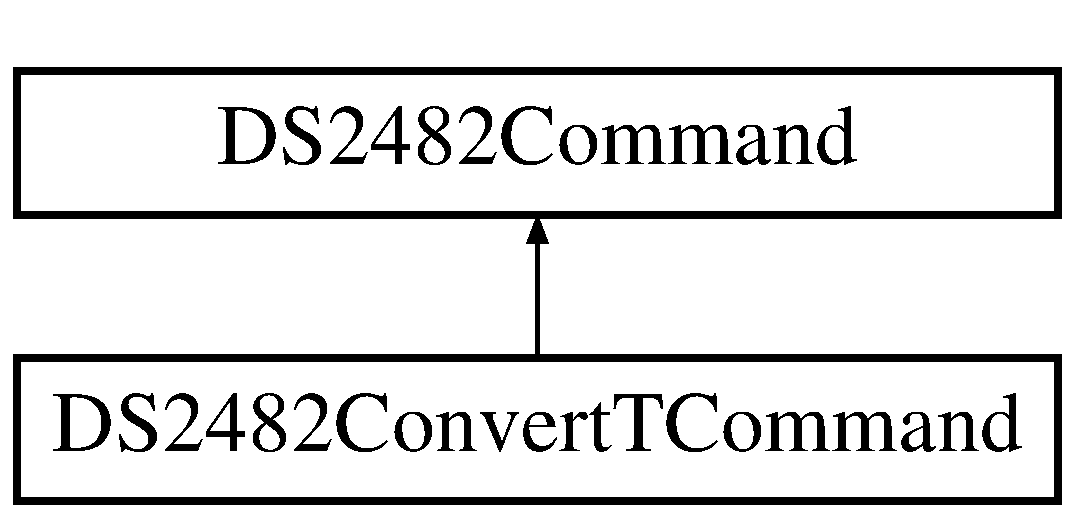
\includegraphics[height=2.000000cm]{class_d_s2482_convert_t_command}
\end{center}
\end{figure}
\subsection*{Public Member Functions}
\begin{DoxyCompactItemize}
\item 
\mbox{\hyperlink{class_d_s2482_convert_t_command}{D\+S2482\+Convert\+T\+Command}} \& \mbox{\hyperlink{class_d_s2482_convert_t_command_a1813c4f607fceab23e6cd1797db8cf8f}{with\+Conversion\+Size}} (int value)
\begin{DoxyCompactList}\small\item\em Sets the conversion size in bits. Default is C\+O\+N\+V\+E\+R\+S\+I\+O\+N\+\_\+12\+B\+IT. \end{DoxyCompactList}\item 
\mbox{\Hypertarget{class_d_s2482_convert_t_command_aef705b42ffe4a90f35ddc11ca713893a}\label{class_d_s2482_convert_t_command_aef705b42ffe4a90f35ddc11ca713893a}} 
\mbox{\hyperlink{class_d_s2482_convert_t_command}{D\+S2482\+Convert\+T\+Command}} \& \mbox{\hyperlink{class_d_s2482_convert_t_command_aef705b42ffe4a90f35ddc11ca713893a}{with\+Parasitic\+Power}} (bool value=true)
\begin{DoxyCompactList}\small\item\em Sets whether to use parasitic power or not. The default is false. \end{DoxyCompactList}\end{DoxyCompactItemize}
\subsection*{Static Public Member Functions}
\begin{DoxyCompactItemize}
\item 
static \mbox{\hyperlink{class_d_s2482_convert_t_command}{D\+S2482\+Convert\+T\+Command}} \& \mbox{\hyperlink{class_d_s2482_convert_t_command_a81579d588ee79fadc7c41cd0bcea37f5}{run}} (\mbox{\hyperlink{class_d_s2482}{D\+S2482}} \&\mbox{\hyperlink{class_d_s2482_command_a54a41fb8a610ef2077f5e5377771aaf3}{parent}}, const \mbox{\hyperlink{class_d_s24821_wire_address}{D\+S24821\+Wire\+Address}} \&addr, std\+::function$<$ void(\mbox{\hyperlink{class_d_s2482_convert_t_command}{D\+S2482\+Convert\+T\+Command}} \&, int status)$>$ completion)
\begin{DoxyCompactList}\small\item\em Sends a C\+O\+N\+V\+E\+R\+T\+\_\+T command -\/ used internally. \end{DoxyCompactList}\end{DoxyCompactItemize}
\subsection*{Friends}
\begin{DoxyCompactItemize}
\item 
\mbox{\Hypertarget{class_d_s2482_convert_t_command_afeaf69274324e8dbeebede05c02d9c18}\label{class_d_s2482_convert_t_command_afeaf69274324e8dbeebede05c02d9c18}} 
class {\bfseries D\+S2482}
\end{DoxyCompactItemize}
\subsection*{Additional Inherited Members}


\subsection{Detailed Description}
Low-\/level class to send a C\+O\+N\+V\+E\+R\+T\+\_\+T command. 

This is a low-\/level command to send a ConvertT command to the D\+S18\+B20s that only does the conversion but does not read the result. You\textquotesingle{}ll typically want to use \mbox{\hyperlink{class_d_s2482_get_temperature_command}{D\+S2482\+Get\+Temperature\+Command}} or \mbox{\hyperlink{class_d_s2482_get_temperature_for_list_command}{D\+S2482\+Get\+Temperature\+For\+List\+Command}} instead.

As with all command objects, you do not typically construct one of these objects. Instead, use the static run method to handle allocating, initializing, and queueing the command. 

\subsection{Member Function Documentation}
\mbox{\Hypertarget{class_d_s2482_convert_t_command_a81579d588ee79fadc7c41cd0bcea37f5}\label{class_d_s2482_convert_t_command_a81579d588ee79fadc7c41cd0bcea37f5}} 
\index{D\+S2482\+Convert\+T\+Command@{D\+S2482\+Convert\+T\+Command}!run@{run}}
\index{run@{run}!D\+S2482\+Convert\+T\+Command@{D\+S2482\+Convert\+T\+Command}}
\subsubsection{\texorpdfstring{run()}{run()}}
{\footnotesize\ttfamily \mbox{\hyperlink{class_d_s2482_convert_t_command}{D\+S2482\+Convert\+T\+Command}} \& D\+S2482\+Convert\+T\+Command\+::run (\begin{DoxyParamCaption}\item[{\mbox{\hyperlink{class_d_s2482}{D\+S2482}} \&}]{parent,  }\item[{const \mbox{\hyperlink{class_d_s24821_wire_address}{D\+S24821\+Wire\+Address}} \&}]{addr,  }\item[{std\+::function$<$ void(\mbox{\hyperlink{class_d_s2482_convert_t_command}{D\+S2482\+Convert\+T\+Command}} \&, int status)$>$}]{completion }\end{DoxyParamCaption})\hspace{0.3cm}{\ttfamily [static]}}



Sends a C\+O\+N\+V\+E\+R\+T\+\_\+T command -\/ used internally. 

Normally you use \mbox{\hyperlink{class_d_s2482_get_temperature_command}{D\+S2482\+Get\+Temperature\+Command}} instead of this low-\/level function. \mbox{\Hypertarget{class_d_s2482_convert_t_command_a1813c4f607fceab23e6cd1797db8cf8f}\label{class_d_s2482_convert_t_command_a1813c4f607fceab23e6cd1797db8cf8f}} 
\index{D\+S2482\+Convert\+T\+Command@{D\+S2482\+Convert\+T\+Command}!with\+Conversion\+Size@{with\+Conversion\+Size}}
\index{with\+Conversion\+Size@{with\+Conversion\+Size}!D\+S2482\+Convert\+T\+Command@{D\+S2482\+Convert\+T\+Command}}
\subsubsection{\texorpdfstring{with\+Conversion\+Size()}{withConversionSize()}}
{\footnotesize\ttfamily \mbox{\hyperlink{class_d_s2482_convert_t_command}{D\+S2482\+Convert\+T\+Command}}\& D\+S2482\+Convert\+T\+Command\+::with\+Conversion\+Size (\begin{DoxyParamCaption}\item[{int}]{value }\end{DoxyParamCaption})\hspace{0.3cm}{\ttfamily [inline]}}



Sets the conversion size in bits. Default is C\+O\+N\+V\+E\+R\+S\+I\+O\+N\+\_\+12\+B\+IT. 


\begin{DoxyParams}{Parameters}
{\em value} & The number of bits the D\+S18\+B20s are configured for. The constants are defined in the \mbox{\hyperlink{class_d_s2482_command}{D\+S2482\+Command}} class and are one of\+: C\+O\+N\+V\+E\+R\+S\+I\+O\+N\+\_\+9\+B\+IT, C\+O\+N\+V\+E\+R\+S\+I\+O\+N\+\_\+10\+B\+IT, C\+O\+N\+V\+E\+R\+S\+I\+O\+N\+\_\+11\+B\+IT, or C\+O\+N\+V\+E\+R\+S\+I\+O\+N\+\_\+12\+B\+IT. At 9 bits, the resolution is 1/2 degrees C. At 12 bits, the resolution is 1/16 degrees C. The factory default hardware setting is 12 bits. Note that you must have use D\+S2482\+Set\+Config to set the conversion size first; just reducing the value in this call without changing the D\+S18\+B20 configuration will result in invalid readings.\\
\hline
\end{DoxyParams}
In the unusual situation that you have sensors of different bit settings, select the largest bit setting. 

The documentation for this class was generated from the following files\+:\begin{DoxyCompactItemize}
\item 
src/D\+S2482-\/\+R\+K.\+h\item 
src/D\+S2482-\/\+R\+K.\+cpp\end{DoxyCompactItemize}

\hypertarget{class_d_s2482_device}{}\section{D\+S2482\+Device Class Reference}
\label{class_d_s2482_device}\index{D\+S2482\+Device@{D\+S2482\+Device}}


Holds the address and temperature for a single D\+S18\+B20 the 1-\/wire bus.  




{\ttfamily \#include $<$D\+S2482-\/\+R\+K.\+h$>$}

\subsection*{Public Member Functions}
\begin{DoxyCompactItemize}
\item 
\mbox{\Hypertarget{class_d_s2482_device_a4a69ea2cd0957ecade28deb98f9ec515}\label{class_d_s2482_device_a4a69ea2cd0957ecade28deb98f9ec515}} 
\mbox{\hyperlink{class_d_s2482_device_a4a69ea2cd0957ecade28deb98f9ec515}{D\+S2482\+Device}} ()
\begin{DoxyCompactList}\small\item\em Constructs an empty \mbox{\hyperlink{class_d_s2482_device}{D\+S2482\+Device}} object. \end{DoxyCompactList}\item 
\mbox{\Hypertarget{class_d_s2482_device_a3fd7f9463d2660fa2feca97d51924de0}\label{class_d_s2482_device_a3fd7f9463d2660fa2feca97d51924de0}} 
virtual \mbox{\hyperlink{class_d_s2482_device_a3fd7f9463d2660fa2feca97d51924de0}{$\sim$\+D\+S2482\+Device}} ()
\begin{DoxyCompactList}\small\item\em Destructor for \mbox{\hyperlink{class_d_s2482_device}{D\+S2482\+Device}}. \end{DoxyCompactList}\item 
\mbox{\hyperlink{class_d_s2482_device_adf7bcc962188f30c285057f28914bf2a}{D\+S2482\+Device}} (const \mbox{\hyperlink{class_d_s24821_wire_address}{D\+S24821\+Wire\+Address}} \&\mbox{\hyperlink{class_d_s2482_device_a83f16b37bc9a89032f9a3e4d096f2e1e}{addr}})
\item 
\mbox{\Hypertarget{class_d_s2482_device_adcff18cd19c99b0c297d9dd70baf6bb7}\label{class_d_s2482_device_adcff18cd19c99b0c297d9dd70baf6bb7}} 
\mbox{\hyperlink{class_d_s2482_device_adcff18cd19c99b0c297d9dd70baf6bb7}{D\+S2482\+Device}} (const \mbox{\hyperlink{class_d_s2482_device}{D\+S2482\+Device}} \&other)
\begin{DoxyCompactList}\small\item\em Constructs a \mbox{\hyperlink{class_d_s2482_device}{D\+S2482\+Device}} object from another \mbox{\hyperlink{class_d_s2482_device}{D\+S2482\+Device}} (copy constructor). \end{DoxyCompactList}\item 
\mbox{\Hypertarget{class_d_s2482_device_ab3f97de99e7502b3779df956ad51a330}\label{class_d_s2482_device_ab3f97de99e7502b3779df956ad51a330}} 
\mbox{\hyperlink{class_d_s2482_device}{D\+S2482\+Device}} \& \mbox{\hyperlink{class_d_s2482_device_ab3f97de99e7502b3779df956ad51a330}{operator=}} (const \mbox{\hyperlink{class_d_s2482_device}{D\+S2482\+Device}} \&other)
\begin{DoxyCompactList}\small\item\em Copies another \mbox{\hyperlink{class_d_s2482_device}{D\+S2482\+Device}} object values into this one. \end{DoxyCompactList}\item 
String \mbox{\hyperlink{class_d_s2482_device_aba40245ed81c0995c4c2de97ca5de032}{to\+String}} () const
\item 
\mbox{\Hypertarget{class_d_s2482_device_a2b496358123002cfa29a0f8c08ae10d9}\label{class_d_s2482_device_a2b496358123002cfa29a0f8c08ae10d9}} 
void \mbox{\hyperlink{class_d_s2482_device_a2b496358123002cfa29a0f8c08ae10d9}{clear}} ()
\begin{DoxyCompactList}\small\item\em Clears the address, temperature, and valid flags. \end{DoxyCompactList}\item 
float \mbox{\hyperlink{class_d_s2482_device_a62d317b9ec8b672fbeb8c16fa480ddd7}{get\+TemperatureC}} () const
\begin{DoxyCompactList}\small\item\em Gets the temperature in degrees Celsius. \end{DoxyCompactList}\item 
float \mbox{\hyperlink{class_d_s2482_device_a61ede76341c0c6409ae3faecadbd1545}{get\+TemperatureF}} () const
\begin{DoxyCompactList}\small\item\em Gets the temperature in degrees Fahrenheit. \end{DoxyCompactList}\item 
void \mbox{\hyperlink{class_d_s2482_device_af1891adba72138aa522b258cc6d4026e}{set\+TemperatureC}} (float value)
\begin{DoxyCompactList}\small\item\em Sets the temperature in degrees Celsius. \end{DoxyCompactList}\item 
bool \mbox{\hyperlink{class_d_s2482_device_a50eeb974bc88c7f2a1c3133a9f1cf8bb}{get\+Valid}} () const
\begin{DoxyCompactList}\small\item\em Gets the valid flag for this temperature reading. \end{DoxyCompactList}\item 
\mbox{\Hypertarget{class_d_s2482_device_a5910ab0269dfbbeb399ab38213ca7e49}\label{class_d_s2482_device_a5910ab0269dfbbeb399ab38213ca7e49}} 
void \mbox{\hyperlink{class_d_s2482_device_a5910ab0269dfbbeb399ab38213ca7e49}{set\+Valid}} (bool value)
\begin{DoxyCompactList}\small\item\em Sets the valid flag. \end{DoxyCompactList}\item 
\mbox{\Hypertarget{class_d_s2482_device_afaef2b385d85c7dd8dd78e6b86cb5751}\label{class_d_s2482_device_afaef2b385d85c7dd8dd78e6b86cb5751}} 
\mbox{\hyperlink{class_d_s24821_wire_address}{D\+S24821\+Wire\+Address}} \mbox{\hyperlink{class_d_s2482_device_afaef2b385d85c7dd8dd78e6b86cb5751}{get\+Address}} () const
\begin{DoxyCompactList}\small\item\em Gets a copy of the \mbox{\hyperlink{class_d_s24821_wire_address}{D\+S24821\+Wire\+Address}} address. \end{DoxyCompactList}\item 
void \mbox{\hyperlink{class_d_s2482_device_a97f56684da4d9b9670d21041e5da15f4}{set\+Address}} (const \mbox{\hyperlink{class_d_s24821_wire_address}{D\+S24821\+Wire\+Address}} \&\mbox{\hyperlink{class_d_s2482_device_a83f16b37bc9a89032f9a3e4d096f2e1e}{addr}})
\begin{DoxyCompactList}\small\item\em Sets the 1-\/wire address. \end{DoxyCompactList}\end{DoxyCompactItemize}
\subsection*{Protected Attributes}
\begin{DoxyCompactItemize}
\item 
\mbox{\Hypertarget{class_d_s2482_device_a83f16b37bc9a89032f9a3e4d096f2e1e}\label{class_d_s2482_device_a83f16b37bc9a89032f9a3e4d096f2e1e}} 
\mbox{\hyperlink{class_d_s24821_wire_address}{D\+S24821\+Wire\+Address}} \mbox{\hyperlink{class_d_s2482_device_a83f16b37bc9a89032f9a3e4d096f2e1e}{addr}}
\begin{DoxyCompactList}\small\item\em The 1-\/wire address (8 bytes) \end{DoxyCompactList}\item 
\mbox{\Hypertarget{class_d_s2482_device_ac69467f7fd8e076dffc9c0fc6c728dd0}\label{class_d_s2482_device_ac69467f7fd8e076dffc9c0fc6c728dd0}} 
float \mbox{\hyperlink{class_d_s2482_device_ac69467f7fd8e076dffc9c0fc6c728dd0}{temperatureC}}
\begin{DoxyCompactList}\small\item\em The last temperature in degrees Celsius. \end{DoxyCompactList}\item 
\mbox{\Hypertarget{class_d_s2482_device_ae07027aa55716a3bf25ae28379aa48ce}\label{class_d_s2482_device_ae07027aa55716a3bf25ae28379aa48ce}} 
bool \mbox{\hyperlink{class_d_s2482_device_ae07027aa55716a3bf25ae28379aa48ce}{valid}}
\begin{DoxyCompactList}\small\item\em True if the last temperature read was successful. \end{DoxyCompactList}\end{DoxyCompactItemize}


\subsection{Detailed Description}
Holds the address and temperature for a single D\+S18\+B20 the 1-\/wire bus. 

This hold the address, the last temperature, and whether the last retrieval was valid or not. 

\subsection{Constructor \& Destructor Documentation}
\mbox{\Hypertarget{class_d_s2482_device_adf7bcc962188f30c285057f28914bf2a}\label{class_d_s2482_device_adf7bcc962188f30c285057f28914bf2a}} 
\index{D\+S2482\+Device@{D\+S2482\+Device}!D\+S2482\+Device@{D\+S2482\+Device}}
\index{D\+S2482\+Device@{D\+S2482\+Device}!D\+S2482\+Device@{D\+S2482\+Device}}
\subsubsection{\texorpdfstring{D\+S2482\+Device()}{DS2482Device()}}
{\footnotesize\ttfamily D\+S2482\+Device\+::\+D\+S2482\+Device (\begin{DoxyParamCaption}\item[{const \mbox{\hyperlink{class_d_s24821_wire_address}{D\+S24821\+Wire\+Address}} \&}]{addr }\end{DoxyParamCaption})}

Constructs a \mbox{\hyperlink{class_d_s2482_device}{D\+S2482\+Device}} object from a 1-\/wire address \mbox{\hyperlink{class_d_s24821_wire_address}{D\+S24821\+Wire\+Address}}. 

\subsection{Member Function Documentation}
\mbox{\Hypertarget{class_d_s2482_device_a62d317b9ec8b672fbeb8c16fa480ddd7}\label{class_d_s2482_device_a62d317b9ec8b672fbeb8c16fa480ddd7}} 
\index{D\+S2482\+Device@{D\+S2482\+Device}!get\+TemperatureC@{get\+TemperatureC}}
\index{get\+TemperatureC@{get\+TemperatureC}!D\+S2482\+Device@{D\+S2482\+Device}}
\subsubsection{\texorpdfstring{get\+Temperature\+C()}{getTemperatureC()}}
{\footnotesize\ttfamily float D\+S2482\+Device\+::get\+TemperatureC (\begin{DoxyParamCaption}{ }\end{DoxyParamCaption}) const\hspace{0.3cm}{\ttfamily [inline]}}



Gets the temperature in degrees Celsius. 

Note that the resolution depends on the conversion bit settings. It ranges from 1/2 degree (9-\/bit) to 1/16 degree (12-\/bit) \mbox{\Hypertarget{class_d_s2482_device_a61ede76341c0c6409ae3faecadbd1545}\label{class_d_s2482_device_a61ede76341c0c6409ae3faecadbd1545}} 
\index{D\+S2482\+Device@{D\+S2482\+Device}!get\+TemperatureF@{get\+TemperatureF}}
\index{get\+TemperatureF@{get\+TemperatureF}!D\+S2482\+Device@{D\+S2482\+Device}}
\subsubsection{\texorpdfstring{get\+Temperature\+F()}{getTemperatureF()}}
{\footnotesize\ttfamily float D\+S2482\+Device\+::get\+TemperatureF (\begin{DoxyParamCaption}{ }\end{DoxyParamCaption}) const\hspace{0.3cm}{\ttfamily [inline]}}



Gets the temperature in degrees Fahrenheit. 

The D\+S18\+B20 uses Celsius internally, so the resolution is reflected in that. The degrees F is the actual converted value and may have more decimal places. \mbox{\Hypertarget{class_d_s2482_device_a50eeb974bc88c7f2a1c3133a9f1cf8bb}\label{class_d_s2482_device_a50eeb974bc88c7f2a1c3133a9f1cf8bb}} 
\index{D\+S2482\+Device@{D\+S2482\+Device}!get\+Valid@{get\+Valid}}
\index{get\+Valid@{get\+Valid}!D\+S2482\+Device@{D\+S2482\+Device}}
\subsubsection{\texorpdfstring{get\+Valid()}{getValid()}}
{\footnotesize\ttfamily bool D\+S2482\+Device\+::get\+Valid (\begin{DoxyParamCaption}{ }\end{DoxyParamCaption}) const\hspace{0.3cm}{\ttfamily [inline]}}



Gets the valid flag for this temperature reading. 

When getting a list of temperatures using \mbox{\hyperlink{class_d_s2482_get_temperature_for_list_command}{D\+S2482\+Get\+Temperature\+For\+List\+Command}}, it\textquotesingle{}s possible that not every sensor will return a value. The get\+Valid allows you to figure out which ones are valid. \mbox{\Hypertarget{class_d_s2482_device_a97f56684da4d9b9670d21041e5da15f4}\label{class_d_s2482_device_a97f56684da4d9b9670d21041e5da15f4}} 
\index{D\+S2482\+Device@{D\+S2482\+Device}!set\+Address@{set\+Address}}
\index{set\+Address@{set\+Address}!D\+S2482\+Device@{D\+S2482\+Device}}
\subsubsection{\texorpdfstring{set\+Address()}{setAddress()}}
{\footnotesize\ttfamily void D\+S2482\+Device\+::set\+Address (\begin{DoxyParamCaption}\item[{const \mbox{\hyperlink{class_d_s24821_wire_address}{D\+S24821\+Wire\+Address}} \&}]{addr }\end{DoxyParamCaption})\hspace{0.3cm}{\ttfamily [inline]}}



Sets the 1-\/wire address. 


\begin{DoxyParams}{Parameters}
{\em addr} & The address to set.\\
\hline
\end{DoxyParams}
The addr is copied, so it does not need to be preserved after this call completes. \mbox{\Hypertarget{class_d_s2482_device_af1891adba72138aa522b258cc6d4026e}\label{class_d_s2482_device_af1891adba72138aa522b258cc6d4026e}} 
\index{D\+S2482\+Device@{D\+S2482\+Device}!set\+TemperatureC@{set\+TemperatureC}}
\index{set\+TemperatureC@{set\+TemperatureC}!D\+S2482\+Device@{D\+S2482\+Device}}
\subsubsection{\texorpdfstring{set\+Temperature\+C()}{setTemperatureC()}}
{\footnotesize\ttfamily void D\+S2482\+Device\+::set\+TemperatureC (\begin{DoxyParamCaption}\item[{float}]{value }\end{DoxyParamCaption})\hspace{0.3cm}{\ttfamily [inline]}}



Sets the temperature in degrees Celsius. 


\begin{DoxyParams}{Parameters}
{\em value} & Temperature in degrees Celsius (as a float) \\
\hline
\end{DoxyParams}
\mbox{\Hypertarget{class_d_s2482_device_aba40245ed81c0995c4c2de97ca5de032}\label{class_d_s2482_device_aba40245ed81c0995c4c2de97ca5de032}} 
\index{D\+S2482\+Device@{D\+S2482\+Device}!to\+String@{to\+String}}
\index{to\+String@{to\+String}!D\+S2482\+Device@{D\+S2482\+Device}}
\subsubsection{\texorpdfstring{to\+String()}{toString()}}
{\footnotesize\ttfamily String D\+S2482\+Device\+::to\+String (\begin{DoxyParamCaption}{ }\end{DoxyParamCaption}) const}

Returns a string representation of this object including the address, temperature, and valid flag. 

The documentation for this class was generated from the following files\+:\begin{DoxyCompactItemize}
\item 
src/D\+S2482-\/\+R\+K.\+h\item 
src/D\+S2482-\/\+R\+K.\+cpp\end{DoxyCompactItemize}

\hypertarget{class_d_s2482_device_list}{}\section{D\+S2482\+Device\+List Class Reference}
\label{class_d_s2482_device_list}\index{D\+S2482\+Device\+List@{D\+S2482\+Device\+List}}


Holds an array of \mbox{\hyperlink{class_d_s2482_device}{D\+S2482\+Device}} objects.  




{\ttfamily \#include $<$D\+S2482-\/\+R\+K.\+h$>$}

Inheritance diagram for D\+S2482\+Device\+List\+:\begin{figure}[H]
\begin{center}
\leavevmode
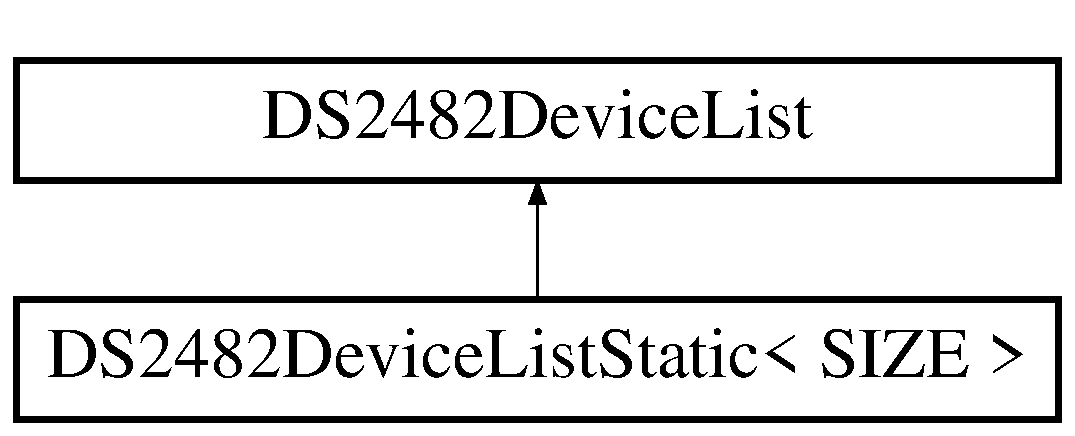
\includegraphics[height=2.000000cm]{class_d_s2482_device_list}
\end{center}
\end{figure}
\subsection*{Public Member Functions}
\begin{DoxyCompactItemize}
\item 
\mbox{\Hypertarget{class_d_s2482_device_list_a86b3c60a954e4410fccc03f77e3942fd}\label{class_d_s2482_device_list_a86b3c60a954e4410fccc03f77e3942fd}} 
\mbox{\hyperlink{class_d_s2482_device_list_a86b3c60a954e4410fccc03f77e3942fd}{D\+S2482\+Device\+List}} (\mbox{\hyperlink{class_d_s2482_device}{D\+S2482\+Device}} $\ast$\mbox{\hyperlink{class_d_s2482_device_list_a37b73673e20f29e7544d5292617815b2}{devices}}, size\+\_\+t \mbox{\hyperlink{class_d_s2482_device_list_a88e117c26f150a9930dd5b65d5733b69}{device\+Max}})
\begin{DoxyCompactList}\small\item\em Constructs a \mbox{\hyperlink{class_d_s2482_device_list}{D\+S2482\+Device\+List}} object with an array of \mbox{\hyperlink{class_d_s2482_device}{D\+S2482\+Device}} objects. \end{DoxyCompactList}\item 
\mbox{\Hypertarget{class_d_s2482_device_list_a7404b545d1704d84a0662255aa3ffe90}\label{class_d_s2482_device_list_a7404b545d1704d84a0662255aa3ffe90}} 
virtual \mbox{\hyperlink{class_d_s2482_device_list_a7404b545d1704d84a0662255aa3ffe90}{$\sim$\+D\+S2482\+Device\+List}} ()
\begin{DoxyCompactList}\small\item\em Destructor for \mbox{\hyperlink{class_d_s2482_device_list}{D\+S2482\+Device\+List}}. \end{DoxyCompactList}\item 
bool \mbox{\hyperlink{class_d_s2482_device_list_a86c4f24502b9cb73376a6b102bb27f52}{add\+Address}} (const \mbox{\hyperlink{class_d_s24821_wire_address}{D\+S24821\+Wire\+Address}} \&addr)
\begin{DoxyCompactList}\small\item\em Adds a \mbox{\hyperlink{class_d_s24821_wire_address}{D\+S24821\+Wire\+Address}} to the device list. \end{DoxyCompactList}\item 
\mbox{\Hypertarget{class_d_s2482_device_list_a8051df54601455c0ba9573b3089b3091}\label{class_d_s2482_device_list_a8051df54601455c0ba9573b3089b3091}} 
void \mbox{\hyperlink{class_d_s2482_device_list_a8051df54601455c0ba9573b3089b3091}{clear}} ()
\begin{DoxyCompactList}\small\item\em Clears add of the objects in the array. \end{DoxyCompactList}\item 
void \mbox{\hyperlink{class_d_s2482_device_list_a2775548aa0394724d64a73f48b93f938}{clear\+Valid}} ()
\begin{DoxyCompactList}\small\item\em Clears all of the valid values in the array. \end{DoxyCompactList}\item 
\mbox{\hyperlink{class_d_s24821_wire_address}{D\+S24821\+Wire\+Address}} \mbox{\hyperlink{class_d_s2482_device_list_a6957f627e300638c9d25313664bc65e1}{get\+Address\+By\+Index}} (size\+\_\+t ii)
\begin{DoxyCompactList}\small\item\em Gets the 1-\/wire address of a device in list by index. \end{DoxyCompactList}\item 
\mbox{\hyperlink{class_d_s2482_device}{D\+S2482\+Device}} \& \mbox{\hyperlink{class_d_s2482_device_list_af135ad9891b100429037bb4101ae7ba6}{get\+Device\+By\+Index}} (size\+\_\+t ii)
\begin{DoxyCompactList}\small\item\em Gets the \mbox{\hyperlink{class_d_s2482_device}{D\+S2482\+Device}} of a device in list by index. \end{DoxyCompactList}\item 
const \mbox{\hyperlink{class_d_s2482_device}{D\+S2482\+Device}} \& \mbox{\hyperlink{class_d_s2482_device_list_a8063e2911399c2f957f05d9e41bad9fa}{get\+Device\+By\+Index}} (size\+\_\+t ii) const
\begin{DoxyCompactList}\small\item\em Gets the \mbox{\hyperlink{class_d_s2482_device}{D\+S2482\+Device}} of a device in list by index. \end{DoxyCompactList}\item 
size\+\_\+t \mbox{\hyperlink{class_d_s2482_device_list_aa7fdfbd1db3a6f22aff1135e7a566666}{get\+Device\+Count}} ()
\begin{DoxyCompactList}\small\item\em Returns the number of devices in the list (devices that have been added) \end{DoxyCompactList}\item 
size\+\_\+t \mbox{\hyperlink{class_d_s2482_device_list_a20680f2eeb04a5db9f0e82d8ceff872e}{get\+Device\+Max}} ()
\begin{DoxyCompactList}\small\item\em Returns the maximum number of devices that can be added, based on the size of the array. \end{DoxyCompactList}\end{DoxyCompactItemize}
\subsection*{Protected Attributes}
\begin{DoxyCompactItemize}
\item 
\mbox{\Hypertarget{class_d_s2482_device_list_a37b73673e20f29e7544d5292617815b2}\label{class_d_s2482_device_list_a37b73673e20f29e7544d5292617815b2}} 
\mbox{\hyperlink{class_d_s2482_device}{D\+S2482\+Device}} $\ast$ \mbox{\hyperlink{class_d_s2482_device_list_a37b73673e20f29e7544d5292617815b2}{devices}}
\begin{DoxyCompactList}\small\item\em The array of device objects. \end{DoxyCompactList}\item 
\mbox{\Hypertarget{class_d_s2482_device_list_adf94f4f9e2287e70b4b249991ddb059e}\label{class_d_s2482_device_list_adf94f4f9e2287e70b4b249991ddb059e}} 
size\+\_\+t \mbox{\hyperlink{class_d_s2482_device_list_adf94f4f9e2287e70b4b249991ddb059e}{device\+Count}}
\begin{DoxyCompactList}\small\item\em The number of devices currently in the list (0 = none, 1 = one, ...) \end{DoxyCompactList}\item 
\mbox{\Hypertarget{class_d_s2482_device_list_a88e117c26f150a9930dd5b65d5733b69}\label{class_d_s2482_device_list_a88e117c26f150a9930dd5b65d5733b69}} 
size\+\_\+t \mbox{\hyperlink{class_d_s2482_device_list_a88e117c26f150a9930dd5b65d5733b69}{device\+Max}}
\begin{DoxyCompactList}\small\item\em The maximum number of objects in the array. \end{DoxyCompactList}\end{DoxyCompactItemize}


\subsection{Detailed Description}
Holds an array of \mbox{\hyperlink{class_d_s2482_device}{D\+S2482\+Device}} objects. 

Normally you will use \mbox{\hyperlink{class_d_s2482_device_list_static}{D\+S2482\+Device\+List\+Static}}, below, instead of instantiating this object directly.

This class does not allocate memory; you pass in a buffer and length and it keeps track of the number of devices in the list. Note that device\+Max is in number of \mbox{\hyperlink{class_d_s2482_device}{D\+S2482\+Device}} objects; the actual size in bytes is 16 times that. 

\subsection{Member Function Documentation}
\mbox{\Hypertarget{class_d_s2482_device_list_a86c4f24502b9cb73376a6b102bb27f52}\label{class_d_s2482_device_list_a86c4f24502b9cb73376a6b102bb27f52}} 
\index{D\+S2482\+Device\+List@{D\+S2482\+Device\+List}!add\+Address@{add\+Address}}
\index{add\+Address@{add\+Address}!D\+S2482\+Device\+List@{D\+S2482\+Device\+List}}
\subsubsection{\texorpdfstring{add\+Address()}{addAddress()}}
{\footnotesize\ttfamily bool D\+S2482\+Device\+List\+::add\+Address (\begin{DoxyParamCaption}\item[{const \mbox{\hyperlink{class_d_s24821_wire_address}{D\+S24821\+Wire\+Address}} \&}]{addr }\end{DoxyParamCaption})}



Adds a \mbox{\hyperlink{class_d_s24821_wire_address}{D\+S24821\+Wire\+Address}} to the device list. 


\begin{DoxyParams}{Parameters}
{\em addr} & The 1-\/wire address to add. addr is copied.\\
\hline
\end{DoxyParams}
\begin{DoxyReturn}{Returns}
true if the address was added or false if the device list is full. 
\end{DoxyReturn}
\mbox{\Hypertarget{class_d_s2482_device_list_a2775548aa0394724d64a73f48b93f938}\label{class_d_s2482_device_list_a2775548aa0394724d64a73f48b93f938}} 
\index{D\+S2482\+Device\+List@{D\+S2482\+Device\+List}!clear\+Valid@{clear\+Valid}}
\index{clear\+Valid@{clear\+Valid}!D\+S2482\+Device\+List@{D\+S2482\+Device\+List}}
\subsubsection{\texorpdfstring{clear\+Valid()}{clearValid()}}
{\footnotesize\ttfamily void D\+S2482\+Device\+List\+::clear\+Valid (\begin{DoxyParamCaption}{ }\end{DoxyParamCaption})}



Clears all of the valid values in the array. 

This is done before reading temperatures using D\+S24821\+Get\+Temperature\+For\+List\+Command. \mbox{\Hypertarget{class_d_s2482_device_list_a6957f627e300638c9d25313664bc65e1}\label{class_d_s2482_device_list_a6957f627e300638c9d25313664bc65e1}} 
\index{D\+S2482\+Device\+List@{D\+S2482\+Device\+List}!get\+Address\+By\+Index@{get\+Address\+By\+Index}}
\index{get\+Address\+By\+Index@{get\+Address\+By\+Index}!D\+S2482\+Device\+List@{D\+S2482\+Device\+List}}
\subsubsection{\texorpdfstring{get\+Address\+By\+Index()}{getAddressByIndex()}}
{\footnotesize\ttfamily \mbox{\hyperlink{class_d_s24821_wire_address}{D\+S24821\+Wire\+Address}} D\+S2482\+Device\+List\+::get\+Address\+By\+Index (\begin{DoxyParamCaption}\item[{size\+\_\+t}]{ii }\end{DoxyParamCaption})\hspace{0.3cm}{\ttfamily [inline]}}



Gets the 1-\/wire address of a device in list by index. 


\begin{DoxyParams}{Parameters}
{\em ii} & The index to retrieve (0 is the first element)\\
\hline
\end{DoxyParams}
\begin{DoxyReturn}{Returns}
The address as a \mbox{\hyperlink{class_d_s24821_wire_address}{D\+S24821\+Wire\+Address}} (copied) 
\end{DoxyReturn}
\mbox{\Hypertarget{class_d_s2482_device_list_af135ad9891b100429037bb4101ae7ba6}\label{class_d_s2482_device_list_af135ad9891b100429037bb4101ae7ba6}} 
\index{D\+S2482\+Device\+List@{D\+S2482\+Device\+List}!get\+Device\+By\+Index@{get\+Device\+By\+Index}}
\index{get\+Device\+By\+Index@{get\+Device\+By\+Index}!D\+S2482\+Device\+List@{D\+S2482\+Device\+List}}
\subsubsection{\texorpdfstring{get\+Device\+By\+Index()}{getDeviceByIndex()}\hspace{0.1cm}{\footnotesize\ttfamily [1/2]}}
{\footnotesize\ttfamily \mbox{\hyperlink{class_d_s2482_device}{D\+S2482\+Device}}\& D\+S2482\+Device\+List\+::get\+Device\+By\+Index (\begin{DoxyParamCaption}\item[{size\+\_\+t}]{ii }\end{DoxyParamCaption})\hspace{0.3cm}{\ttfamily [inline]}}



Gets the \mbox{\hyperlink{class_d_s2482_device}{D\+S2482\+Device}} of a device in list by index. 


\begin{DoxyParams}{Parameters}
{\em ii} & The index to retrieve (0 is the first element)\\
\hline
\end{DoxyParams}
\begin{DoxyReturn}{Returns}
The \mbox{\hyperlink{class_d_s2482_device}{D\+S2482\+Device}} object (the actual object reference, not copied) 
\end{DoxyReturn}
\mbox{\Hypertarget{class_d_s2482_device_list_a8063e2911399c2f957f05d9e41bad9fa}\label{class_d_s2482_device_list_a8063e2911399c2f957f05d9e41bad9fa}} 
\index{D\+S2482\+Device\+List@{D\+S2482\+Device\+List}!get\+Device\+By\+Index@{get\+Device\+By\+Index}}
\index{get\+Device\+By\+Index@{get\+Device\+By\+Index}!D\+S2482\+Device\+List@{D\+S2482\+Device\+List}}
\subsubsection{\texorpdfstring{get\+Device\+By\+Index()}{getDeviceByIndex()}\hspace{0.1cm}{\footnotesize\ttfamily [2/2]}}
{\footnotesize\ttfamily const \mbox{\hyperlink{class_d_s2482_device}{D\+S2482\+Device}}\& D\+S2482\+Device\+List\+::get\+Device\+By\+Index (\begin{DoxyParamCaption}\item[{size\+\_\+t}]{ii }\end{DoxyParamCaption}) const\hspace{0.3cm}{\ttfamily [inline]}}



Gets the \mbox{\hyperlink{class_d_s2482_device}{D\+S2482\+Device}} of a device in list by index. 


\begin{DoxyParams}{Parameters}
{\em ii} & The index to retrieve (0 is the first element)\\
\hline
\end{DoxyParams}
\begin{DoxyReturn}{Returns}
The \mbox{\hyperlink{class_d_s2482_device}{D\+S2482\+Device}} object (the actual object reference, not copied) as a const object that can\textquotesingle{}t be modified.
\end{DoxyReturn}
Note that \mbox{\hyperlink{class_d_s2482_device}{D\+S2482\+Device}} supports the copy operator and copy constructor so it\textquotesingle{}s easy to make your own copy of it. \mbox{\Hypertarget{class_d_s2482_device_list_aa7fdfbd1db3a6f22aff1135e7a566666}\label{class_d_s2482_device_list_aa7fdfbd1db3a6f22aff1135e7a566666}} 
\index{D\+S2482\+Device\+List@{D\+S2482\+Device\+List}!get\+Device\+Count@{get\+Device\+Count}}
\index{get\+Device\+Count@{get\+Device\+Count}!D\+S2482\+Device\+List@{D\+S2482\+Device\+List}}
\subsubsection{\texorpdfstring{get\+Device\+Count()}{getDeviceCount()}}
{\footnotesize\ttfamily size\+\_\+t D\+S2482\+Device\+List\+::get\+Device\+Count (\begin{DoxyParamCaption}{ }\end{DoxyParamCaption})\hspace{0.3cm}{\ttfamily [inline]}}



Returns the number of devices in the list (devices that have been added) 

\begin{DoxyReturn}{Returns}
The number of added devices (0 = none, 1 = one, ...) 
\end{DoxyReturn}
\mbox{\Hypertarget{class_d_s2482_device_list_a20680f2eeb04a5db9f0e82d8ceff872e}\label{class_d_s2482_device_list_a20680f2eeb04a5db9f0e82d8ceff872e}} 
\index{D\+S2482\+Device\+List@{D\+S2482\+Device\+List}!get\+Device\+Max@{get\+Device\+Max}}
\index{get\+Device\+Max@{get\+Device\+Max}!D\+S2482\+Device\+List@{D\+S2482\+Device\+List}}
\subsubsection{\texorpdfstring{get\+Device\+Max()}{getDeviceMax()}}
{\footnotesize\ttfamily size\+\_\+t D\+S2482\+Device\+List\+::get\+Device\+Max (\begin{DoxyParamCaption}{ }\end{DoxyParamCaption})\hspace{0.3cm}{\ttfamily [inline]}}



Returns the maximum number of devices that can be added, based on the size of the array. 

\begin{DoxyReturn}{Returns}
The maximum number of devices that can be added
\end{DoxyReturn}
If \mbox{\hyperlink{class_d_s2482_device_list_aa7fdfbd1db3a6f22aff1135e7a566666}{get\+Device\+Count()}} == \mbox{\hyperlink{class_d_s2482_device_list_a20680f2eeb04a5db9f0e82d8ceff872e}{get\+Device\+Max()}} then the list is full and no more can be added. 

The documentation for this class was generated from the following files\+:\begin{DoxyCompactItemize}
\item 
src/D\+S2482-\/\+R\+K.\+h\item 
src/D\+S2482-\/\+R\+K.\+cpp\end{DoxyCompactItemize}

\hypertarget{class_d_s2482_device_list_static}{}\section{D\+S2482\+Device\+List\+Static$<$ S\+I\+ZE $>$ Class Template Reference}
\label{class_d_s2482_device_list_static}\index{D\+S2482\+Device\+List\+Static$<$ S\+I\+Z\+E $>$@{D\+S2482\+Device\+List\+Static$<$ S\+I\+Z\+E $>$}}


Holds an array of \mbox{\hyperlink{class_d_s2482_device}{D\+S2482\+Device}} objects of a given size.  




{\ttfamily \#include $<$D\+S2482-\/\+R\+K.\+h$>$}

Inheritance diagram for D\+S2482\+Device\+List\+Static$<$ S\+I\+ZE $>$\+:\begin{figure}[H]
\begin{center}
\leavevmode
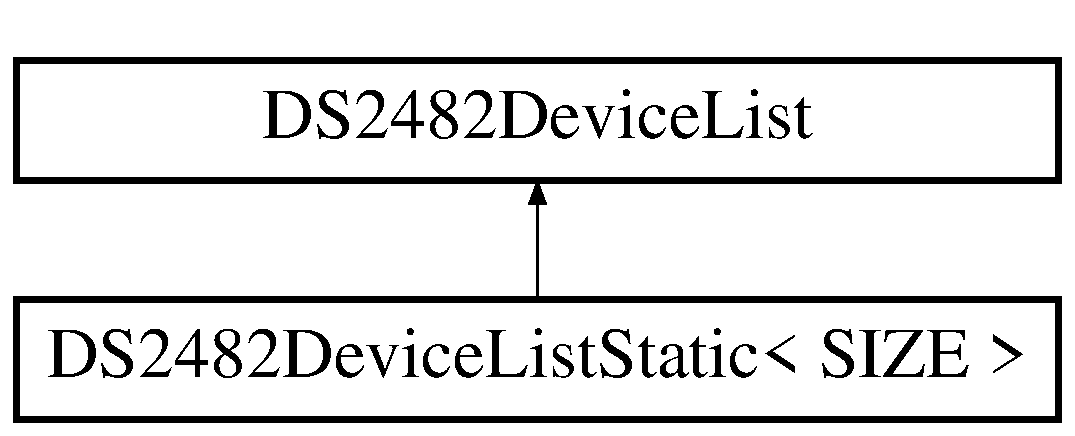
\includegraphics[height=2.000000cm]{class_d_s2482_device_list_static}
\end{center}
\end{figure}
\subsection*{Public Member Functions}
\begin{DoxyCompactItemize}
\item 
\mbox{\Hypertarget{class_d_s2482_device_list_static_ae3709f01bf5902dbeaf00a55772cdc32}\label{class_d_s2482_device_list_static_ae3709f01bf5902dbeaf00a55772cdc32}} 
\mbox{\hyperlink{class_d_s2482_device_list_static_ae3709f01bf5902dbeaf00a55772cdc32}{D\+S2482\+Device\+List\+Static}} ()
\begin{DoxyCompactList}\small\item\em Constructs a static list of devices. \end{DoxyCompactList}\end{DoxyCompactItemize}
\subsection*{Additional Inherited Members}


\subsection{Detailed Description}
\subsubsection*{template$<$size\+\_\+t S\+I\+ZE$>$\newline
class D\+S2482\+Device\+List\+Static$<$ S\+I\+Z\+E $>$}

Holds an array of \mbox{\hyperlink{class_d_s2482_device}{D\+S2482\+Device}} objects of a given size. 

You normally use this class to allocate the array on the heap, stack, or as a class member. You need to know the maximum size in order to use this; the actual number of devices can be less than the maximum size.

The overhead is 16 bytes for each device. Note that size is in number of devices, not bytes.

It\textquotesingle{}s typically used like this\+:

D\+S2482\+Device\+List\+Static$<$10$>$ device\+List;

This allocates a variable device\+List that can hold up to 10 devices. You can include a device list as a global variable, local variable (stack-\/allocated), a class member variable, or on the heap. 

The documentation for this class was generated from the following file\+:\begin{DoxyCompactItemize}
\item 
src/D\+S2482-\/\+R\+K.\+h\end{DoxyCompactItemize}

\hypertarget{class_d_s2482_device_reset}{}\section{D\+S2482\+Device\+Reset Class Reference}
\label{class_d_s2482_device_reset}\index{D\+S2482\+Device\+Reset@{D\+S2482\+Device\+Reset}}


Resets the \mbox{\hyperlink{class_d_s2482}{D\+S2482}}.  




{\ttfamily \#include $<$D\+S2482-\/\+R\+K.\+h$>$}

Inheritance diagram for D\+S2482\+Device\+Reset\+:\begin{figure}[H]
\begin{center}
\leavevmode
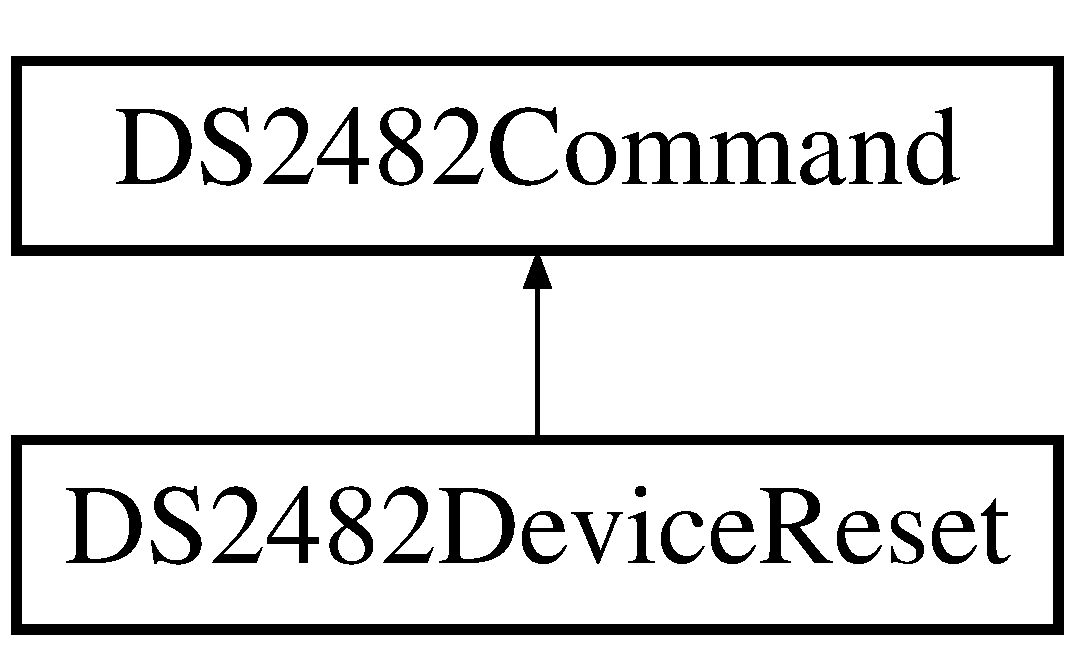
\includegraphics[height=2.000000cm]{class_d_s2482_device_reset}
\end{center}
\end{figure}
\subsection*{Static Public Member Functions}
\begin{DoxyCompactItemize}
\item 
static \mbox{\hyperlink{class_d_s2482_device_reset}{D\+S2482\+Device\+Reset}} \& \mbox{\hyperlink{class_d_s2482_device_reset_a4250bda2cf91a9c21c9ac4844e05689b}{run}} (\mbox{\hyperlink{class_d_s2482}{D\+S2482}} \&\mbox{\hyperlink{class_d_s2482_command_a54a41fb8a610ef2077f5e5377771aaf3}{parent}}, std\+::function$<$ void(\mbox{\hyperlink{class_d_s2482_device_reset}{D\+S2482\+Device\+Reset}} \&, int status)$>$ completion)
\begin{DoxyCompactList}\small\item\em Resets the \mbox{\hyperlink{class_d_s2482}{D\+S2482}}. \end{DoxyCompactList}\end{DoxyCompactItemize}
\subsection*{Friends}
\begin{DoxyCompactItemize}
\item 
\mbox{\Hypertarget{class_d_s2482_device_reset_afeaf69274324e8dbeebede05c02d9c18}\label{class_d_s2482_device_reset_afeaf69274324e8dbeebede05c02d9c18}} 
class {\bfseries D\+S2482}
\end{DoxyCompactItemize}
\subsection*{Additional Inherited Members}


\subsection{Detailed Description}
Resets the \mbox{\hyperlink{class_d_s2482}{D\+S2482}}. 

As with all command objects, you do not typically construct one of these objects. Instead, use the static run method to handle allocating, initializing, and queueing the command. 

\subsection{Member Function Documentation}
\mbox{\Hypertarget{class_d_s2482_device_reset_a4250bda2cf91a9c21c9ac4844e05689b}\label{class_d_s2482_device_reset_a4250bda2cf91a9c21c9ac4844e05689b}} 
\index{D\+S2482\+Device\+Reset@{D\+S2482\+Device\+Reset}!run@{run}}
\index{run@{run}!D\+S2482\+Device\+Reset@{D\+S2482\+Device\+Reset}}
\subsubsection{\texorpdfstring{run()}{run()}}
{\footnotesize\ttfamily \mbox{\hyperlink{class_d_s2482_device_reset}{D\+S2482\+Device\+Reset}} \& D\+S2482\+Device\+Reset\+::run (\begin{DoxyParamCaption}\item[{\mbox{\hyperlink{class_d_s2482}{D\+S2482}} \&}]{parent,  }\item[{std\+::function$<$ void(\mbox{\hyperlink{class_d_s2482_device_reset}{D\+S2482\+Device\+Reset}} \&, int status)$>$}]{completion }\end{DoxyParamCaption})\hspace{0.3cm}{\ttfamily [static]}}



Resets the \mbox{\hyperlink{class_d_s2482}{D\+S2482}}. 


\begin{DoxyParams}{Parameters}
{\em parent} & The \mbox{\hyperlink{class_d_s2482}{D\+S2482}} you want to send the command to.\\
\hline
{\em completion} & The completion handler lambda function. status is the result status of the call; if \mbox{\hyperlink{class_d_s2482_command_a8ffcf84807c97928dbfc61d75788e32b}{D\+S2482\+Command\+::\+R\+E\+S\+U\+L\+T\+\_\+\+D\+O\+NE}} then the call succeeded.\\
\hline
\end{DoxyParams}
This call executes asynchronously. The completion function is called when complete or an error occurs. 

The documentation for this class was generated from the following files\+:\begin{DoxyCompactItemize}
\item 
src/D\+S2482-\/\+R\+K.\+h\item 
src/D\+S2482-\/\+R\+K.\+cpp\end{DoxyCompactItemize}

\hypertarget{class_d_s2482_get_temperature_command}{}\section{D\+S2482\+Get\+Temperature\+Command Class Reference}
\label{class_d_s2482_get_temperature_command}\index{D\+S2482\+Get\+Temperature\+Command@{D\+S2482\+Get\+Temperature\+Command}}


Gets the temperature of a single sensor.  




{\ttfamily \#include $<$D\+S2482-\/\+R\+K.\+h$>$}

Inheritance diagram for D\+S2482\+Get\+Temperature\+Command\+:\begin{figure}[H]
\begin{center}
\leavevmode
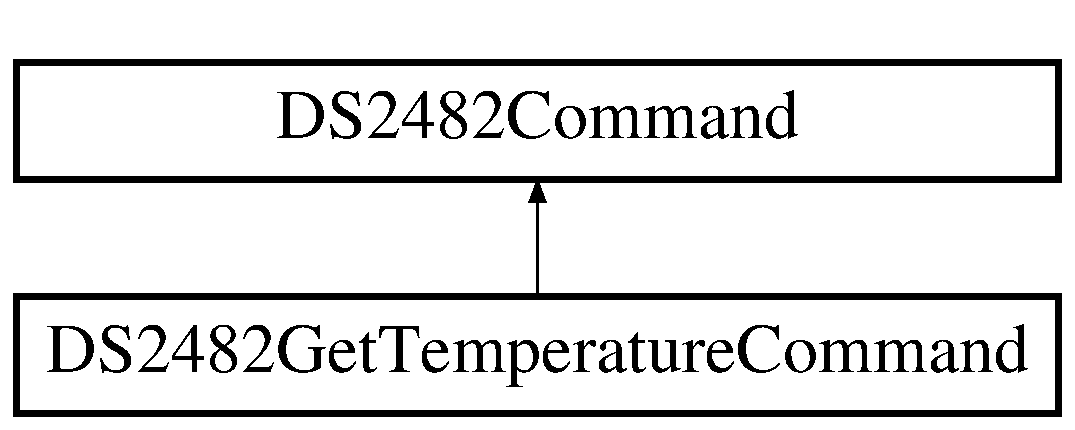
\includegraphics[height=2.000000cm]{class_d_s2482_get_temperature_command}
\end{center}
\end{figure}
\subsection*{Public Member Functions}
\begin{DoxyCompactItemize}
\item 
\mbox{\Hypertarget{class_d_s2482_get_temperature_command_a49764ff0b2607839893d2362e6b894c2}\label{class_d_s2482_get_temperature_command_a49764ff0b2607839893d2362e6b894c2}} 
\mbox{\hyperlink{class_d_s2482_get_temperature_command}{D\+S2482\+Get\+Temperature\+Command}} \& \mbox{\hyperlink{class_d_s2482_get_temperature_command_a49764ff0b2607839893d2362e6b894c2}{with\+Max\+Retries}} (size\+\_\+t value)
\begin{DoxyCompactList}\small\item\em Sets the number of times to retry reading the temperature. Default is 3. \end{DoxyCompactList}\item 
\mbox{\hyperlink{class_d_s2482_get_temperature_command}{D\+S2482\+Get\+Temperature\+Command}} \& \mbox{\hyperlink{class_d_s2482_get_temperature_command_a74bf428300575cfc62e57bbdb5d358ac}{with\+Conversion\+Size}} (int value)
\begin{DoxyCompactList}\small\item\em Sets the conversion size in bits. Default is C\+O\+N\+V\+E\+R\+S\+I\+O\+N\+\_\+12\+B\+IT. \end{DoxyCompactList}\item 
\mbox{\Hypertarget{class_d_s2482_get_temperature_command_a69481de9ee23a9c8c46d724fffc8eff7}\label{class_d_s2482_get_temperature_command_a69481de9ee23a9c8c46d724fffc8eff7}} 
\mbox{\hyperlink{class_d_s2482_get_temperature_command}{D\+S2482\+Get\+Temperature\+Command}} \& \mbox{\hyperlink{class_d_s2482_get_temperature_command_a69481de9ee23a9c8c46d724fffc8eff7}{with\+Parasitic\+Power}} (bool value=true)
\begin{DoxyCompactList}\small\item\em Sets whether to use parasitic power or not. The default is false. \end{DoxyCompactList}\item 
size\+\_\+t \mbox{\hyperlink{class_d_s2482_get_temperature_command_a39a243094572d16385d8ef2ae5180d1f}{get\+Num\+Retries}} () const
\begin{DoxyCompactList}\small\item\em Gets the total number of retries. \end{DoxyCompactList}\end{DoxyCompactItemize}
\subsection*{Static Public Member Functions}
\begin{DoxyCompactItemize}
\item 
static float \mbox{\hyperlink{class_d_s2482_get_temperature_command_af5778f4b03a65c8dc1290516ac73fe92}{convert\+Temp}} (const uint8\+\_\+t $\ast$scratchpad, int conversion\+Size)
\begin{DoxyCompactList}\small\item\em Converts the 16-\/bit scratchpad temperature into a float (degrees C) \end{DoxyCompactList}\item 
static \mbox{\hyperlink{class_d_s2482_get_temperature_command}{D\+S2482\+Get\+Temperature\+Command}} \& \mbox{\hyperlink{class_d_s2482_get_temperature_command_a91c9ee5048047d209e3dd1effa1ba179}{run}} (\mbox{\hyperlink{class_d_s2482}{D\+S2482}} \&\mbox{\hyperlink{class_d_s2482_command_a54a41fb8a610ef2077f5e5377771aaf3}{parent}}, const \mbox{\hyperlink{class_d_s24821_wire_address}{D\+S24821\+Wire\+Address}} \&addr, std\+::function$<$ void(\mbox{\hyperlink{class_d_s2482_get_temperature_command}{D\+S2482\+Get\+Temperature\+Command}} \&, int status, float tempC)$>$ completion)
\begin{DoxyCompactList}\small\item\em Gets the temperatures for a D\+S18\+B20 sensor on the 1-\/wire bus. \end{DoxyCompactList}\end{DoxyCompactItemize}
\subsection*{Friends}
\begin{DoxyCompactItemize}
\item 
\mbox{\Hypertarget{class_d_s2482_get_temperature_command_afeaf69274324e8dbeebede05c02d9c18}\label{class_d_s2482_get_temperature_command_afeaf69274324e8dbeebede05c02d9c18}} 
class {\bfseries D\+S2482}
\end{DoxyCompactItemize}
\subsection*{Additional Inherited Members}


\subsection{Detailed Description}
Gets the temperature of a single sensor. 

See also \mbox{\hyperlink{class_d_s2482_get_temperature_for_list_command}{D\+S2482\+Get\+Temperature\+For\+List\+Command}} for an efficient way to read multiple sensors on a single 1-\/wire bus.

As with all command objects, you do not typically construct one of these objects. Instead, use the static run method to handle allocating, initializing, and queueing the command. 

\subsection{Member Function Documentation}
\mbox{\Hypertarget{class_d_s2482_get_temperature_command_af5778f4b03a65c8dc1290516ac73fe92}\label{class_d_s2482_get_temperature_command_af5778f4b03a65c8dc1290516ac73fe92}} 
\index{D\+S2482\+Get\+Temperature\+Command@{D\+S2482\+Get\+Temperature\+Command}!convert\+Temp@{convert\+Temp}}
\index{convert\+Temp@{convert\+Temp}!D\+S2482\+Get\+Temperature\+Command@{D\+S2482\+Get\+Temperature\+Command}}
\subsubsection{\texorpdfstring{convert\+Temp()}{convertTemp()}}
{\footnotesize\ttfamily float D\+S2482\+Get\+Temperature\+Command\+::convert\+Temp (\begin{DoxyParamCaption}\item[{const uint8\+\_\+t $\ast$}]{scratchpad,  }\item[{int}]{conversion\+Size }\end{DoxyParamCaption})\hspace{0.3cm}{\ttfamily [static]}}



Converts the 16-\/bit scratchpad temperature into a float (degrees C) 

It takes a conversion size because the least signficant bits in 9-\/11 bit operation are not zereoed -\/ they contain random values. The conversion\+Size is used to mask them off to 0. \mbox{\Hypertarget{class_d_s2482_get_temperature_command_a39a243094572d16385d8ef2ae5180d1f}\label{class_d_s2482_get_temperature_command_a39a243094572d16385d8ef2ae5180d1f}} 
\index{D\+S2482\+Get\+Temperature\+Command@{D\+S2482\+Get\+Temperature\+Command}!get\+Num\+Retries@{get\+Num\+Retries}}
\index{get\+Num\+Retries@{get\+Num\+Retries}!D\+S2482\+Get\+Temperature\+Command@{D\+S2482\+Get\+Temperature\+Command}}
\subsubsection{\texorpdfstring{get\+Num\+Retries()}{getNumRetries()}}
{\footnotesize\ttfamily size\+\_\+t D\+S2482\+Get\+Temperature\+Command\+::get\+Num\+Retries (\begin{DoxyParamCaption}{ }\end{DoxyParamCaption}) const\hspace{0.3cm}{\ttfamily [inline]}}



Gets the total number of retries. 

This should be 0 most of the time when the sensor was read successfully the first time. \mbox{\Hypertarget{class_d_s2482_get_temperature_command_a91c9ee5048047d209e3dd1effa1ba179}\label{class_d_s2482_get_temperature_command_a91c9ee5048047d209e3dd1effa1ba179}} 
\index{D\+S2482\+Get\+Temperature\+Command@{D\+S2482\+Get\+Temperature\+Command}!run@{run}}
\index{run@{run}!D\+S2482\+Get\+Temperature\+Command@{D\+S2482\+Get\+Temperature\+Command}}
\subsubsection{\texorpdfstring{run()}{run()}}
{\footnotesize\ttfamily \mbox{\hyperlink{class_d_s2482_get_temperature_command}{D\+S2482\+Get\+Temperature\+Command}} \& D\+S2482\+Get\+Temperature\+Command\+::run (\begin{DoxyParamCaption}\item[{\mbox{\hyperlink{class_d_s2482}{D\+S2482}} \&}]{parent,  }\item[{const \mbox{\hyperlink{class_d_s24821_wire_address}{D\+S24821\+Wire\+Address}} \&}]{addr,  }\item[{std\+::function$<$ void(\mbox{\hyperlink{class_d_s2482_get_temperature_command}{D\+S2482\+Get\+Temperature\+Command}} \&, int status, float tempC)$>$}]{completion }\end{DoxyParamCaption})\hspace{0.3cm}{\ttfamily [static]}}



Gets the temperatures for a D\+S18\+B20 sensor on the 1-\/wire bus. 


\begin{DoxyParams}{Parameters}
{\em parent} & The \mbox{\hyperlink{class_d_s2482}{D\+S2482}} you want to send the command to. If it\textquotesingle{}s a D\+S2482\+\_\+800, make sure you set the channel as well.\\
\hline
{\em addr} & The address you want to read. For a single drop 1-\/wire bus you can pass a newly constructed empty \mbox{\hyperlink{class_d_s24821_wire_address}{D\+S24821\+Wire\+Address}} object which causes S\+K\+I\+P\+\_\+\+R\+OM to be used instead of M\+A\+T\+C\+H\+\_\+\+R\+OM this eliminates the need to search the bus and more efficiently reads when there is only one D\+S18\+B20 on the 1-\/wire bus.\\
\hline
{\em completion} & The completion handler lambda function. status is the result status of the call; if \mbox{\hyperlink{class_d_s2482_command_a8ffcf84807c97928dbfc61d75788e32b}{D\+S2482\+Command\+::\+R\+E\+S\+U\+L\+T\+\_\+\+D\+O\+NE}} then the call succeeded.\\
\hline
\end{DoxyParams}
This call executes asynchronously. The completion function is called when complete or an error occurs. The execution time depends on the number of bits. \mbox{\Hypertarget{class_d_s2482_get_temperature_command_a74bf428300575cfc62e57bbdb5d358ac}\label{class_d_s2482_get_temperature_command_a74bf428300575cfc62e57bbdb5d358ac}} 
\index{D\+S2482\+Get\+Temperature\+Command@{D\+S2482\+Get\+Temperature\+Command}!with\+Conversion\+Size@{with\+Conversion\+Size}}
\index{with\+Conversion\+Size@{with\+Conversion\+Size}!D\+S2482\+Get\+Temperature\+Command@{D\+S2482\+Get\+Temperature\+Command}}
\subsubsection{\texorpdfstring{with\+Conversion\+Size()}{withConversionSize()}}
{\footnotesize\ttfamily \mbox{\hyperlink{class_d_s2482_get_temperature_command}{D\+S2482\+Get\+Temperature\+Command}}\& D\+S2482\+Get\+Temperature\+Command\+::with\+Conversion\+Size (\begin{DoxyParamCaption}\item[{int}]{value }\end{DoxyParamCaption})\hspace{0.3cm}{\ttfamily [inline]}}



Sets the conversion size in bits. Default is C\+O\+N\+V\+E\+R\+S\+I\+O\+N\+\_\+12\+B\+IT. 


\begin{DoxyParams}{Parameters}
{\em value} & The number of bits the D\+S18\+B20s are configured for. The constants are defined in the \mbox{\hyperlink{class_d_s2482_command}{D\+S2482\+Command}} class and are one of\+: C\+O\+N\+V\+E\+R\+S\+I\+O\+N\+\_\+9\+B\+IT, C\+O\+N\+V\+E\+R\+S\+I\+O\+N\+\_\+10\+B\+IT, C\+O\+N\+V\+E\+R\+S\+I\+O\+N\+\_\+11\+B\+IT, or C\+O\+N\+V\+E\+R\+S\+I\+O\+N\+\_\+12\+B\+IT. At 9 bits, the resolution is 1/2 degrees C. At 12 bits, the resolution is 1/16 degrees C. The factory default hardware setting is 12 bits. Note that you must have use D\+S2482\+Set\+Config to set the conversion size first; just reducing the value in this call without changing the D\+S18\+B20 configuration will result in invalid readings.\\
\hline
\end{DoxyParams}
In the unusual situation that you have sensors of different bit settings, select the largest bit setting. 

The documentation for this class was generated from the following files\+:\begin{DoxyCompactItemize}
\item 
src/D\+S2482-\/\+R\+K.\+h\item 
src/D\+S2482-\/\+R\+K.\+cpp\end{DoxyCompactItemize}

\hypertarget{class_d_s2482_get_temperature_for_list_command}{}\section{D\+S2482\+Get\+Temperature\+For\+List\+Command Class Reference}
\label{class_d_s2482_get_temperature_for_list_command}\index{D\+S2482\+Get\+Temperature\+For\+List\+Command@{D\+S2482\+Get\+Temperature\+For\+List\+Command}}


Gets the temperatures for multiple D\+S18\+B20 sensors on a single bus.  




{\ttfamily \#include $<$D\+S2482-\/\+R\+K.\+h$>$}

Inheritance diagram for D\+S2482\+Get\+Temperature\+For\+List\+Command\+:\begin{figure}[H]
\begin{center}
\leavevmode
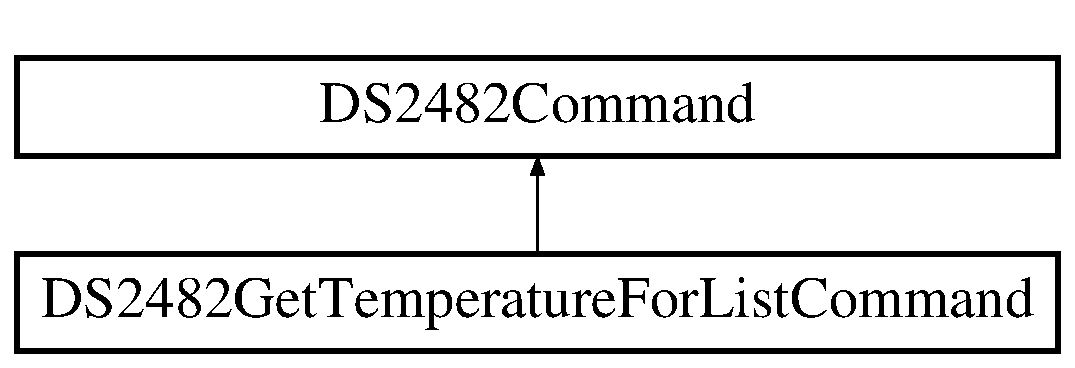
\includegraphics[height=2.000000cm]{class_d_s2482_get_temperature_for_list_command}
\end{center}
\end{figure}
\subsection*{Public Member Functions}
\begin{DoxyCompactItemize}
\item 
\mbox{\Hypertarget{class_d_s2482_get_temperature_for_list_command_abf3514034c3423dac4a17a02ea9928b8}\label{class_d_s2482_get_temperature_for_list_command_abf3514034c3423dac4a17a02ea9928b8}} 
\mbox{\hyperlink{class_d_s2482_get_temperature_for_list_command}{D\+S2482\+Get\+Temperature\+For\+List\+Command}} \& \mbox{\hyperlink{class_d_s2482_get_temperature_for_list_command_abf3514034c3423dac4a17a02ea9928b8}{with\+Max\+Retries}} (size\+\_\+t value)
\begin{DoxyCompactList}\small\item\em Sets the number of times to retry reading the temperature. Default is 3. \end{DoxyCompactList}\item 
\mbox{\hyperlink{class_d_s2482_get_temperature_for_list_command}{D\+S2482\+Get\+Temperature\+For\+List\+Command}} \& \mbox{\hyperlink{class_d_s2482_get_temperature_for_list_command_a2e9bb74693d3644df1d503a168f7da72}{with\+Conversion\+Size}} (int value)
\begin{DoxyCompactList}\small\item\em Sets the conversion size in bits. Default is C\+O\+N\+V\+E\+R\+S\+I\+O\+N\+\_\+12\+B\+IT. \end{DoxyCompactList}\item 
\mbox{\Hypertarget{class_d_s2482_get_temperature_for_list_command_af1a1456ab9c30f667fcdeeff6091dd33}\label{class_d_s2482_get_temperature_for_list_command_af1a1456ab9c30f667fcdeeff6091dd33}} 
\mbox{\hyperlink{class_d_s2482_get_temperature_for_list_command}{D\+S2482\+Get\+Temperature\+For\+List\+Command}} \& \mbox{\hyperlink{class_d_s2482_get_temperature_for_list_command_af1a1456ab9c30f667fcdeeff6091dd33}{with\+Parasitic\+Power}} (bool value=true)
\begin{DoxyCompactList}\small\item\em Sets whether to use parasitic power or not. The default is false. \end{DoxyCompactList}\item 
size\+\_\+t \mbox{\hyperlink{class_d_s2482_get_temperature_for_list_command_a962f91c29fa4a2a1d5c02ab2f4c120a9}{get\+Num\+Retries}} () const
\begin{DoxyCompactList}\small\item\em Gets the total number of retries across all sensor reads. \end{DoxyCompactList}\end{DoxyCompactItemize}
\subsection*{Static Public Member Functions}
\begin{DoxyCompactItemize}
\item 
static \mbox{\hyperlink{class_d_s2482_get_temperature_for_list_command}{D\+S2482\+Get\+Temperature\+For\+List\+Command}} \& \mbox{\hyperlink{class_d_s2482_get_temperature_for_list_command_ad0895d68b4409b157891b751e740b4fe}{run}} (\mbox{\hyperlink{class_d_s2482}{D\+S2482}} \&\mbox{\hyperlink{class_d_s2482_command_a54a41fb8a610ef2077f5e5377771aaf3}{parent}}, \mbox{\hyperlink{class_d_s2482_device_list}{D\+S2482\+Device\+List}} \&device\+List, std\+::function$<$ void(\mbox{\hyperlink{class_d_s2482_get_temperature_for_list_command}{D\+S2482\+Get\+Temperature\+For\+List\+Command}} \&, int status, \mbox{\hyperlink{class_d_s2482_device_list}{D\+S2482\+Device\+List}} \&device\+List)$>$ completion)
\begin{DoxyCompactList}\small\item\em Gets the temperatures for a number of D\+S18\+B20 sensors on the 1-\/wire bus. \end{DoxyCompactList}\end{DoxyCompactItemize}
\subsection*{Friends}
\begin{DoxyCompactItemize}
\item 
\mbox{\Hypertarget{class_d_s2482_get_temperature_for_list_command_afeaf69274324e8dbeebede05c02d9c18}\label{class_d_s2482_get_temperature_for_list_command_afeaf69274324e8dbeebede05c02d9c18}} 
class {\bfseries D\+S2482}
\end{DoxyCompactItemize}
\subsection*{Additional Inherited Members}


\subsection{Detailed Description}
Gets the temperatures for multiple D\+S18\+B20 sensors on a single bus. 

This is faster than calling \mbox{\hyperlink{class_d_s2482_get_temperature_command}{D\+S2482\+Get\+Temperature\+Command}} for each sensor separately. The reason is that the longest operation, ConvertT, takes 750 milliseconds (for 12-\/bit readings). When you use \mbox{\hyperlink{class_d_s2482_get_temperature_for_list_command}{D\+S2482\+Get\+Temperature\+For\+List\+Command}} ConvertT for all of the sensors on the bus is done at the same time, so you only incur the 750 millisecond time once, regardless of how many sensors are on the bus. The individual readings need to be made for each D\+S18\+B20, but that\textquotesingle{}s fast.

As with all command objects, you do not typically construct one of these objects. Instead, use the static run method to handle allocating, initializing, and queueing the command. 

\subsection{Member Function Documentation}
\mbox{\Hypertarget{class_d_s2482_get_temperature_for_list_command_a962f91c29fa4a2a1d5c02ab2f4c120a9}\label{class_d_s2482_get_temperature_for_list_command_a962f91c29fa4a2a1d5c02ab2f4c120a9}} 
\index{D\+S2482\+Get\+Temperature\+For\+List\+Command@{D\+S2482\+Get\+Temperature\+For\+List\+Command}!get\+Num\+Retries@{get\+Num\+Retries}}
\index{get\+Num\+Retries@{get\+Num\+Retries}!D\+S2482\+Get\+Temperature\+For\+List\+Command@{D\+S2482\+Get\+Temperature\+For\+List\+Command}}
\subsubsection{\texorpdfstring{get\+Num\+Retries()}{getNumRetries()}}
{\footnotesize\ttfamily size\+\_\+t D\+S2482\+Get\+Temperature\+For\+List\+Command\+::get\+Num\+Retries (\begin{DoxyParamCaption}{ }\end{DoxyParamCaption}) const\hspace{0.3cm}{\ttfamily [inline]}}



Gets the total number of retries across all sensor reads. 

This should be 0 most of the time when all sensors were read successfully the first time. \mbox{\Hypertarget{class_d_s2482_get_temperature_for_list_command_ad0895d68b4409b157891b751e740b4fe}\label{class_d_s2482_get_temperature_for_list_command_ad0895d68b4409b157891b751e740b4fe}} 
\index{D\+S2482\+Get\+Temperature\+For\+List\+Command@{D\+S2482\+Get\+Temperature\+For\+List\+Command}!run@{run}}
\index{run@{run}!D\+S2482\+Get\+Temperature\+For\+List\+Command@{D\+S2482\+Get\+Temperature\+For\+List\+Command}}
\subsubsection{\texorpdfstring{run()}{run()}}
{\footnotesize\ttfamily \mbox{\hyperlink{class_d_s2482_get_temperature_for_list_command}{D\+S2482\+Get\+Temperature\+For\+List\+Command}} \& D\+S2482\+Get\+Temperature\+For\+List\+Command\+::run (\begin{DoxyParamCaption}\item[{\mbox{\hyperlink{class_d_s2482}{D\+S2482}} \&}]{parent,  }\item[{\mbox{\hyperlink{class_d_s2482_device_list}{D\+S2482\+Device\+List}} \&}]{device\+List,  }\item[{std\+::function$<$ void(\mbox{\hyperlink{class_d_s2482_get_temperature_for_list_command}{D\+S2482\+Get\+Temperature\+For\+List\+Command}} \&, int status, \mbox{\hyperlink{class_d_s2482_device_list}{D\+S2482\+Device\+List}} \&device\+List)$>$}]{completion }\end{DoxyParamCaption})\hspace{0.3cm}{\ttfamily [static]}}



Gets the temperatures for a number of D\+S18\+B20 sensors on the 1-\/wire bus. 


\begin{DoxyParams}{Parameters}
{\em parent} & The \mbox{\hyperlink{class_d_s2482}{D\+S2482}} you want to send the command to. If it\textquotesingle{}s a D\+S2482\+\_\+800, make sure you set the channel as well.\\
\hline
{\em device\+List} & the \mbox{\hyperlink{class_d_s2482_device_list}{D\+S2482\+Device\+List}} for the devices you want to get the temperatures for\\
\hline
{\em completion} & The completion handler lambda function. status is the result status of the call; if \mbox{\hyperlink{class_d_s2482_command_a8ffcf84807c97928dbfc61d75788e32b}{D\+S2482\+Command\+::\+R\+E\+S\+U\+L\+T\+\_\+\+D\+O\+NE}} then the call succeeded.\\
\hline
\end{DoxyParams}
This is faster than calling \mbox{\hyperlink{class_d_s2482_get_temperature_command}{D\+S2482\+Get\+Temperature\+Command}} for each sensor separately. The reason is that the longest operation, ConvertT, takes 750 milliseconds (for 12-\/bit readings). When you use \mbox{\hyperlink{class_d_s2482_get_temperature_for_list_command}{D\+S2482\+Get\+Temperature\+For\+List\+Command}} ConvertT for all of the sensors on the bus is done at the same time, so you only incur the 750 millisecond time once, regardless of how many sensors are on the bus. The individual readings need to be made for each D\+S18\+B20, but that\textquotesingle{}s fast.

Note that every D\+S18\+B20 on the 1-\/wire bus is commanded to convert their temperature, not just the ones in the device\+List. Only the temperatures for the sensors in the device\+List are retrieved, however.

This call executes asynchronously. The completion function is called when complete or an error occurs. \mbox{\Hypertarget{class_d_s2482_get_temperature_for_list_command_a2e9bb74693d3644df1d503a168f7da72}\label{class_d_s2482_get_temperature_for_list_command_a2e9bb74693d3644df1d503a168f7da72}} 
\index{D\+S2482\+Get\+Temperature\+For\+List\+Command@{D\+S2482\+Get\+Temperature\+For\+List\+Command}!with\+Conversion\+Size@{with\+Conversion\+Size}}
\index{with\+Conversion\+Size@{with\+Conversion\+Size}!D\+S2482\+Get\+Temperature\+For\+List\+Command@{D\+S2482\+Get\+Temperature\+For\+List\+Command}}
\subsubsection{\texorpdfstring{with\+Conversion\+Size()}{withConversionSize()}}
{\footnotesize\ttfamily \mbox{\hyperlink{class_d_s2482_get_temperature_for_list_command}{D\+S2482\+Get\+Temperature\+For\+List\+Command}}\& D\+S2482\+Get\+Temperature\+For\+List\+Command\+::with\+Conversion\+Size (\begin{DoxyParamCaption}\item[{int}]{value }\end{DoxyParamCaption})\hspace{0.3cm}{\ttfamily [inline]}}



Sets the conversion size in bits. Default is C\+O\+N\+V\+E\+R\+S\+I\+O\+N\+\_\+12\+B\+IT. 


\begin{DoxyParams}{Parameters}
{\em value} & The number of bits the D\+S18\+B20s are configured for. The constants are defined in the \mbox{\hyperlink{class_d_s2482_command}{D\+S2482\+Command}} class and are one of\+: C\+O\+N\+V\+E\+R\+S\+I\+O\+N\+\_\+9\+B\+IT, C\+O\+N\+V\+E\+R\+S\+I\+O\+N\+\_\+10\+B\+IT, C\+O\+N\+V\+E\+R\+S\+I\+O\+N\+\_\+11\+B\+IT, or C\+O\+N\+V\+E\+R\+S\+I\+O\+N\+\_\+12\+B\+IT. At 9 bits, the resolution is 1/2 degrees C. At 12 bits, the resolution is 1/16 degrees C. The factory default hardware setting is 12 bits. Note that you must have use D\+S2482\+Set\+Config to set the conversion size first; just reducing the value in this call without changing the D\+S18\+B20 configuration will result in invalid readings.\\
\hline
\end{DoxyParams}
In the unusual situation that you have sensors of different bit settings, select the largest bit setting. 

The documentation for this class was generated from the following files\+:\begin{DoxyCompactItemize}
\item 
src/D\+S2482-\/\+R\+K.\+h\item 
src/D\+S2482-\/\+R\+K.\+cpp\end{DoxyCompactItemize}

\hypertarget{class_d_s2482_match_rom}{}\section{D\+S2482\+Match\+Rom Class Reference}
\label{class_d_s2482_match_rom}\index{D\+S2482\+Match\+Rom@{D\+S2482\+Match\+Rom}}


Low-\/level class to send a M\+A\+T\+C\+H\+\_\+\+R\+OM command. This is used internally by D\+S2482\+Read\+Scratchpad and others.  




{\ttfamily \#include $<$D\+S2482-\/\+R\+K.\+h$>$}

Inheritance diagram for D\+S2482\+Match\+Rom\+:\begin{figure}[H]
\begin{center}
\leavevmode
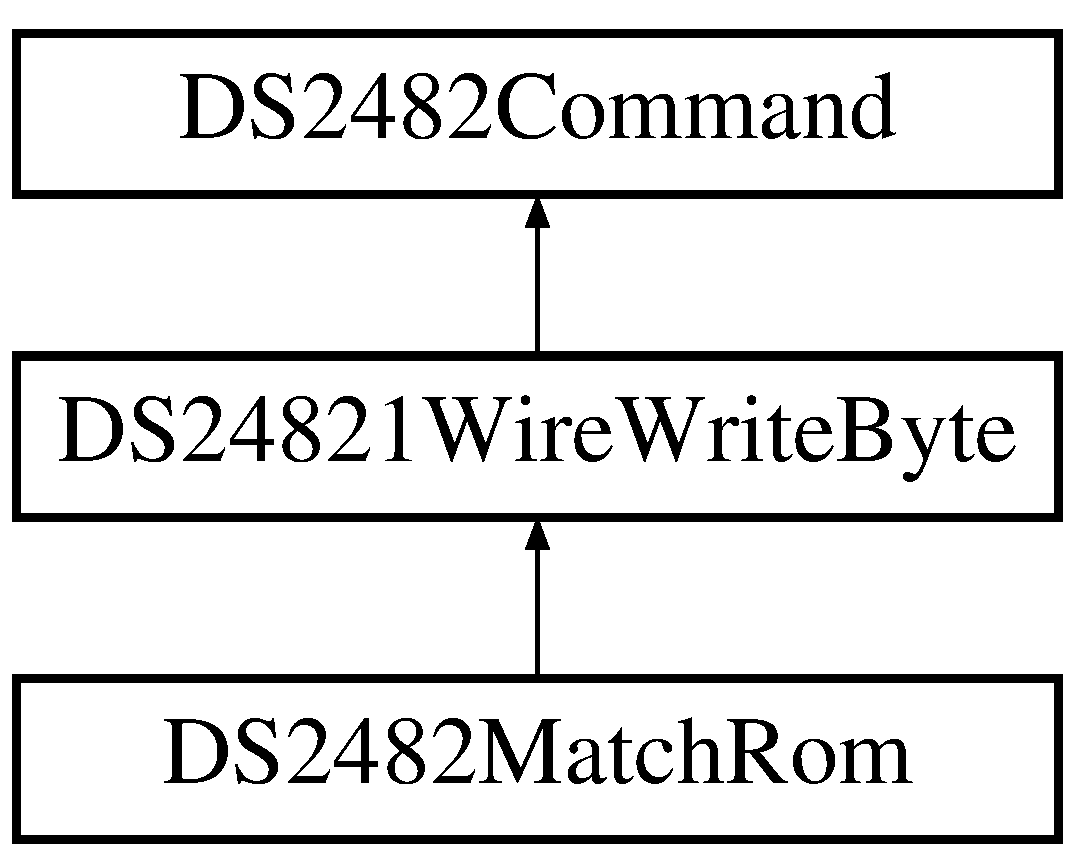
\includegraphics[height=3.000000cm]{class_d_s2482_match_rom}
\end{center}
\end{figure}
\subsection*{Static Public Member Functions}
\begin{DoxyCompactItemize}
\item 
\mbox{\Hypertarget{class_d_s2482_match_rom_acd4303311cf3df03c68d07f9c3a29ff5}\label{class_d_s2482_match_rom_acd4303311cf3df03c68d07f9c3a29ff5}} 
static \mbox{\hyperlink{class_d_s2482_match_rom}{D\+S2482\+Match\+Rom}} \& \mbox{\hyperlink{class_d_s2482_match_rom_acd4303311cf3df03c68d07f9c3a29ff5}{run}} (\mbox{\hyperlink{class_d_s2482}{D\+S2482}} \&\mbox{\hyperlink{class_d_s2482_command_a54a41fb8a610ef2077f5e5377771aaf3}{parent}}, std\+::function$<$ void(\mbox{\hyperlink{class_d_s24821_wire_write_byte}{D\+S24821\+Wire\+Write\+Byte}} \&, int status)$>$ completion)
\begin{DoxyCompactList}\small\item\em Sends a M\+A\+T\+C\+H\+\_\+\+R\+OM command -\/ used internally. \end{DoxyCompactList}\end{DoxyCompactItemize}
\subsection*{Friends}
\begin{DoxyCompactItemize}
\item 
\mbox{\Hypertarget{class_d_s2482_match_rom_afeaf69274324e8dbeebede05c02d9c18}\label{class_d_s2482_match_rom_afeaf69274324e8dbeebede05c02d9c18}} 
class {\bfseries D\+S2482}
\end{DoxyCompactItemize}
\subsection*{Additional Inherited Members}


\subsection{Detailed Description}
Low-\/level class to send a M\+A\+T\+C\+H\+\_\+\+R\+OM command. This is used internally by D\+S2482\+Read\+Scratchpad and others. 

As with all command objects, you do not typically construct one of these objects. Instead, use the static run method to handle allocating, initializing, and queueing the command. 

The documentation for this class was generated from the following files\+:\begin{DoxyCompactItemize}
\item 
src/D\+S2482-\/\+R\+K.\+h\item 
src/D\+S2482-\/\+R\+K.\+cpp\end{DoxyCompactItemize}

\hypertarget{class_d_s2482_read_rom}{}\section{D\+S2482\+Read\+Rom Class Reference}
\label{class_d_s2482_read_rom}\index{D\+S2482\+Read\+Rom@{D\+S2482\+Read\+Rom}}


Low-\/level class to send a R\+E\+A\+D\+\_\+\+R\+OM command.  




{\ttfamily \#include $<$D\+S2482-\/\+R\+K.\+h$>$}

Inheritance diagram for D\+S2482\+Read\+Rom\+:\begin{figure}[H]
\begin{center}
\leavevmode
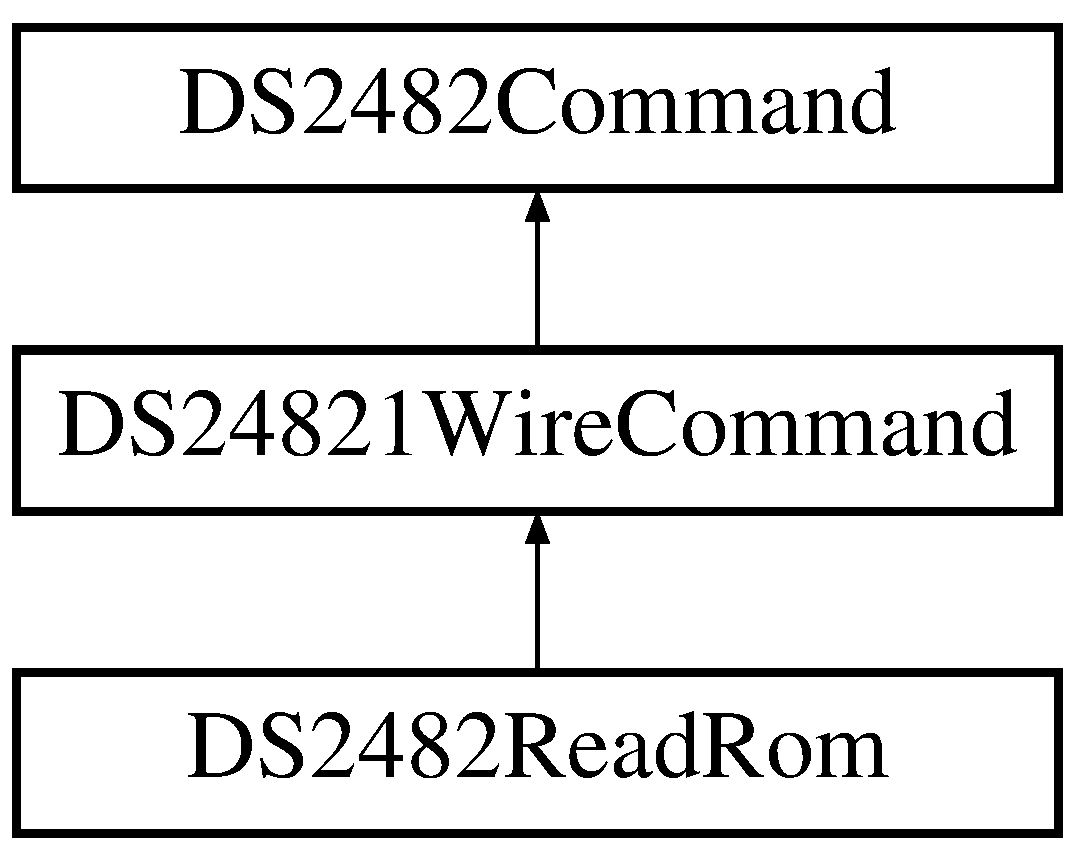
\includegraphics[height=3.000000cm]{class_d_s2482_read_rom}
\end{center}
\end{figure}
\subsection*{Static Public Member Functions}
\begin{DoxyCompactItemize}
\item 
\mbox{\Hypertarget{class_d_s2482_read_rom_a6962376a38dee206044733f1fe6f6153}\label{class_d_s2482_read_rom_a6962376a38dee206044733f1fe6f6153}} 
static \mbox{\hyperlink{class_d_s2482_read_rom}{D\+S2482\+Read\+Rom}} \& \mbox{\hyperlink{class_d_s2482_read_rom_a6962376a38dee206044733f1fe6f6153}{run}} (\mbox{\hyperlink{class_d_s2482}{D\+S2482}} \&\mbox{\hyperlink{class_d_s2482_command_a54a41fb8a610ef2077f5e5377771aaf3}{parent}}, std\+::function$<$ void(\mbox{\hyperlink{class_d_s24821_wire_command}{D\+S24821\+Wire\+Command}} \&, int status)$>$ completion)
\begin{DoxyCompactList}\small\item\em Sends a R\+E\+A\+D\+\_\+\+R\+OM command -\/ used internally. \end{DoxyCompactList}\end{DoxyCompactItemize}
\subsection*{Friends}
\begin{DoxyCompactItemize}
\item 
\mbox{\Hypertarget{class_d_s2482_read_rom_afeaf69274324e8dbeebede05c02d9c18}\label{class_d_s2482_read_rom_afeaf69274324e8dbeebede05c02d9c18}} 
class {\bfseries D\+S2482}
\end{DoxyCompactItemize}
\subsection*{Additional Inherited Members}


\subsection{Detailed Description}
Low-\/level class to send a R\+E\+A\+D\+\_\+\+R\+OM command. 

As with all command objects, you do not typically construct one of these objects. Instead, use the static run method to handle allocating, initializing, and queueing the command. 

The documentation for this class was generated from the following files\+:\begin{DoxyCompactItemize}
\item 
src/D\+S2482-\/\+R\+K.\+h\item 
src/D\+S2482-\/\+R\+K.\+cpp\end{DoxyCompactItemize}

\hypertarget{class_d_s2482_read_scratchpad_command}{}\section{D\+S2482\+Read\+Scratchpad\+Command Class Reference}
\label{class_d_s2482_read_scratchpad_command}\index{D\+S2482\+Read\+Scratchpad\+Command@{D\+S2482\+Read\+Scratchpad\+Command}}


Low-\/level call to read the scratchpad.  




{\ttfamily \#include $<$D\+S2482-\/\+R\+K.\+h$>$}

Inheritance diagram for D\+S2482\+Read\+Scratchpad\+Command\+:\begin{figure}[H]
\begin{center}
\leavevmode
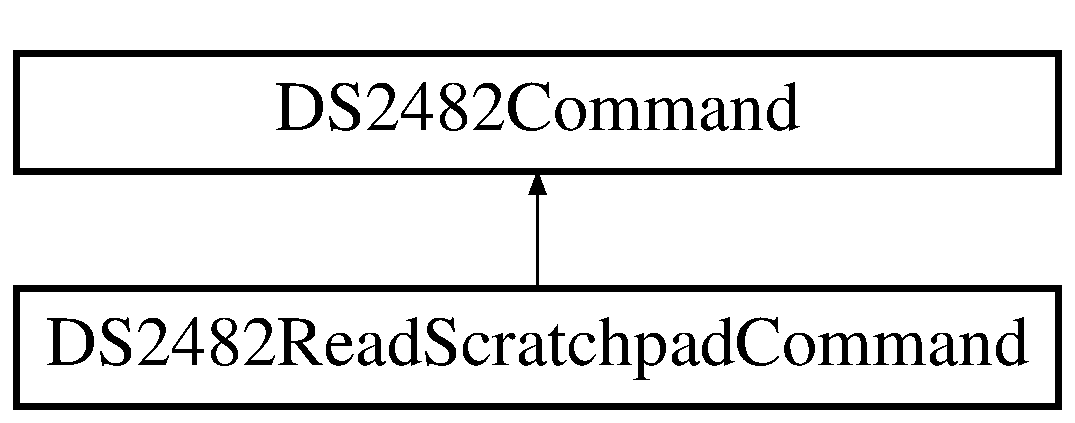
\includegraphics[height=2.000000cm]{class_d_s2482_read_scratchpad_command}
\end{center}
\end{figure}
\subsection*{Public Member Functions}
\begin{DoxyCompactItemize}
\item 
\mbox{\Hypertarget{class_d_s2482_read_scratchpad_command_a816a8806e254ed36e677eb060820e5de}\label{class_d_s2482_read_scratchpad_command_a816a8806e254ed36e677eb060820e5de}} 
\mbox{\hyperlink{class_d_s2482_read_scratchpad_command}{D\+S2482\+Read\+Scratchpad\+Command}} \& \mbox{\hyperlink{class_d_s2482_read_scratchpad_command_a816a8806e254ed36e677eb060820e5de}{with\+Max\+Retries}} (size\+\_\+t value)
\begin{DoxyCompactList}\small\item\em Sets the number of times to retry reading the temperature. Default is 3. \end{DoxyCompactList}\item 
size\+\_\+t \mbox{\hyperlink{class_d_s2482_read_scratchpad_command_a41ec4653739bf4d13351a25800fedb91}{get\+Num\+Retries}} () const
\begin{DoxyCompactList}\small\item\em Gets the total number of retries. \end{DoxyCompactList}\end{DoxyCompactItemize}
\subsection*{Static Public Member Functions}
\begin{DoxyCompactItemize}
\item 
\mbox{\Hypertarget{class_d_s2482_read_scratchpad_command_a863d13d919605916ed21fd7f7ead9d2a}\label{class_d_s2482_read_scratchpad_command_a863d13d919605916ed21fd7f7ead9d2a}} 
static \mbox{\hyperlink{class_d_s2482_read_scratchpad_command}{D\+S2482\+Read\+Scratchpad\+Command}} \& \mbox{\hyperlink{class_d_s2482_read_scratchpad_command_a863d13d919605916ed21fd7f7ead9d2a}{run}} (\mbox{\hyperlink{class_d_s2482}{D\+S2482}} \&\mbox{\hyperlink{class_d_s2482_command_a54a41fb8a610ef2077f5e5377771aaf3}{parent}}, const \mbox{\hyperlink{class_d_s24821_wire_address}{D\+S24821\+Wire\+Address}} \&addr, std\+::function$<$ void(\mbox{\hyperlink{class_d_s2482_read_scratchpad_command}{D\+S2482\+Read\+Scratchpad\+Command}} \&, int status, uint8\+\_\+t $\ast$scratchpad)$>$ completion)
\begin{DoxyCompactList}\small\item\em Sends a R\+E\+A\+D\+\_\+\+S\+C\+R\+A\+T\+C\+H\+P\+AD command -\/ used internally. \end{DoxyCompactList}\end{DoxyCompactItemize}
\subsection*{Friends}
\begin{DoxyCompactItemize}
\item 
\mbox{\Hypertarget{class_d_s2482_read_scratchpad_command_afeaf69274324e8dbeebede05c02d9c18}\label{class_d_s2482_read_scratchpad_command_afeaf69274324e8dbeebede05c02d9c18}} 
class {\bfseries D\+S2482}
\end{DoxyCompactItemize}
\subsection*{Additional Inherited Members}


\subsection{Detailed Description}
Low-\/level call to read the scratchpad. 

The most common use for reading the scratchpad is to get the previously converted temperature value.

You\textquotesingle{}ll typically want to use \mbox{\hyperlink{class_d_s2482_get_temperature_command}{D\+S2482\+Get\+Temperature\+Command}} or \mbox{\hyperlink{class_d_s2482_get_temperature_for_list_command}{D\+S2482\+Get\+Temperature\+For\+List\+Command}} instead which uses \mbox{\hyperlink{class_d_s2482_convert_t_command}{D\+S2482\+Convert\+T\+Command}} and \mbox{\hyperlink{class_d_s2482_read_scratchpad_command}{D\+S2482\+Read\+Scratchpad\+Command}} internally.

As with all command objects, you do not typically construct one of these objects. Instead, use the static run method to handle allocating, initializing, and queueing the command. 

\subsection{Member Function Documentation}
\mbox{\Hypertarget{class_d_s2482_read_scratchpad_command_a41ec4653739bf4d13351a25800fedb91}\label{class_d_s2482_read_scratchpad_command_a41ec4653739bf4d13351a25800fedb91}} 
\index{D\+S2482\+Read\+Scratchpad\+Command@{D\+S2482\+Read\+Scratchpad\+Command}!get\+Num\+Retries@{get\+Num\+Retries}}
\index{get\+Num\+Retries@{get\+Num\+Retries}!D\+S2482\+Read\+Scratchpad\+Command@{D\+S2482\+Read\+Scratchpad\+Command}}
\subsubsection{\texorpdfstring{get\+Num\+Retries()}{getNumRetries()}}
{\footnotesize\ttfamily size\+\_\+t D\+S2482\+Read\+Scratchpad\+Command\+::get\+Num\+Retries (\begin{DoxyParamCaption}{ }\end{DoxyParamCaption}) const\hspace{0.3cm}{\ttfamily [inline]}}



Gets the total number of retries. 

This should be 0 most of the time when the scratchpad read successfully the first time. 

The documentation for this class was generated from the following files\+:\begin{DoxyCompactItemize}
\item 
src/D\+S2482-\/\+R\+K.\+h\item 
src/D\+S2482-\/\+R\+K.\+cpp\end{DoxyCompactItemize}

\hypertarget{class_d_s2482_read_scratchpad_internal}{}\section{D\+S2482\+Read\+Scratchpad\+Internal Class Reference}
\label{class_d_s2482_read_scratchpad_internal}\index{D\+S2482\+Read\+Scratchpad\+Internal@{D\+S2482\+Read\+Scratchpad\+Internal}}


Used internally to do the actual read scratchpad operation.  




{\ttfamily \#include $<$D\+S2482-\/\+R\+K.\+h$>$}

Inheritance diagram for D\+S2482\+Read\+Scratchpad\+Internal\+:\begin{figure}[H]
\begin{center}
\leavevmode
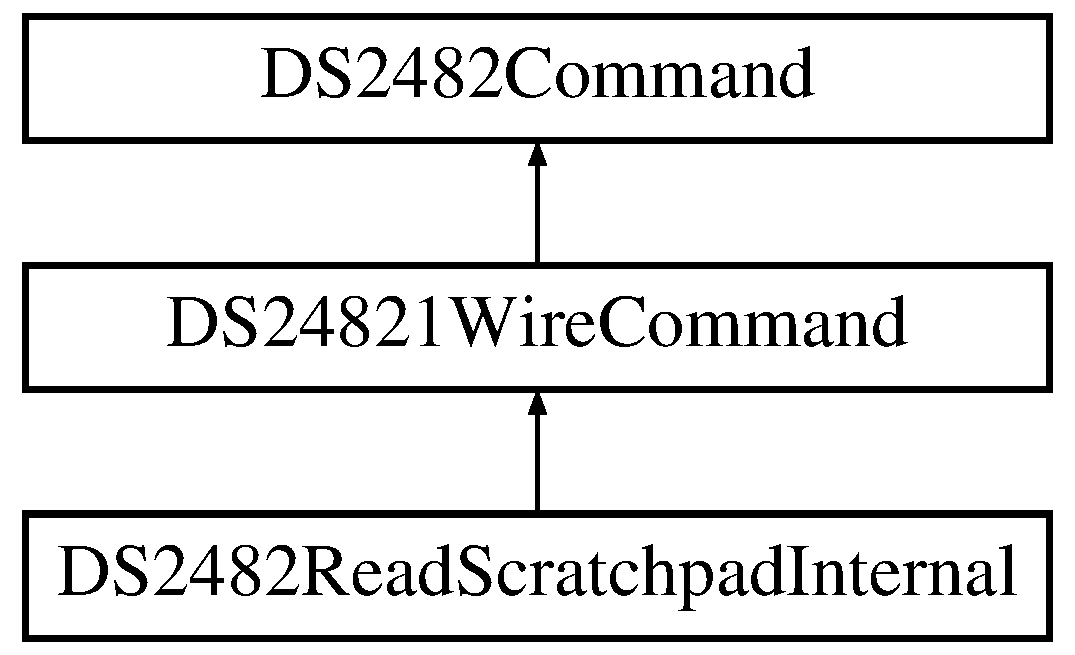
\includegraphics[height=3.000000cm]{class_d_s2482_read_scratchpad_internal}
\end{center}
\end{figure}
\subsection*{Static Public Member Functions}
\begin{DoxyCompactItemize}
\item 
\mbox{\Hypertarget{class_d_s2482_read_scratchpad_internal_a222c1ac367ecdbecb671c99796a4fa26}\label{class_d_s2482_read_scratchpad_internal_a222c1ac367ecdbecb671c99796a4fa26}} 
static \mbox{\hyperlink{class_d_s2482_read_scratchpad_internal}{D\+S2482\+Read\+Scratchpad\+Internal}} \& \mbox{\hyperlink{class_d_s2482_read_scratchpad_internal_a222c1ac367ecdbecb671c99796a4fa26}{run}} (\mbox{\hyperlink{class_d_s2482}{D\+S2482}} \&\mbox{\hyperlink{class_d_s2482_command_a54a41fb8a610ef2077f5e5377771aaf3}{parent}}, std\+::function$<$ void(\mbox{\hyperlink{class_d_s24821_wire_command}{D\+S24821\+Wire\+Command}} \&, int status)$>$ completion)
\begin{DoxyCompactList}\small\item\em Sends a R\+E\+A\+D\+\_\+\+S\+C\+R\+A\+T\+C\+H\+P\+AD command -\/ used internally. \end{DoxyCompactList}\end{DoxyCompactItemize}
\subsection*{Friends}
\begin{DoxyCompactItemize}
\item 
\mbox{\Hypertarget{class_d_s2482_read_scratchpad_internal_afeaf69274324e8dbeebede05c02d9c18}\label{class_d_s2482_read_scratchpad_internal_afeaf69274324e8dbeebede05c02d9c18}} 
class {\bfseries D\+S2482}
\end{DoxyCompactItemize}
\subsection*{Additional Inherited Members}


\subsection{Detailed Description}
Used internally to do the actual read scratchpad operation. 

Normally you\textquotesingle{}d use \mbox{\hyperlink{class_d_s2482_read_scratchpad_command}{D\+S2482\+Read\+Scratchpad\+Command}} that handles setting the address and handling retries.

As with all command objects, you do not typically construct one of these objects. Instead, use the static run method to handle allocating, initializing, and queueing the command. 

The documentation for this class was generated from the following files\+:\begin{DoxyCompactItemize}
\item 
src/D\+S2482-\/\+R\+K.\+h\item 
src/D\+S2482-\/\+R\+K.\+cpp\end{DoxyCompactItemize}

\hypertarget{struct_d_s2482_search_branch_point}{}\section{D\+S2482\+Search\+Branch\+Point Struct Reference}
\label{struct_d_s2482_search_branch_point}\index{D\+S2482\+Search\+Branch\+Point@{D\+S2482\+Search\+Branch\+Point}}


Internal struct used during 1-\/wire bus searches.  




{\ttfamily \#include $<$D\+S2482-\/\+R\+K.\+h$>$}

\subsection*{Data Fields}
\begin{DoxyCompactItemize}
\item 
\mbox{\Hypertarget{struct_d_s2482_search_branch_point_a7038aafda9f63172a1253bfc4268cd9a}\label{struct_d_s2482_search_branch_point_a7038aafda9f63172a1253bfc4268cd9a}} 
\mbox{\hyperlink{class_d_s24821_wire_address}{D\+S24821\+Wire\+Address}} \mbox{\hyperlink{struct_d_s2482_search_branch_point_a7038aafda9f63172a1253bfc4268cd9a}{addr}}
\begin{DoxyCompactList}\small\item\em The 1-\/wire address being searched. \end{DoxyCompactList}\item 
\mbox{\Hypertarget{struct_d_s2482_search_branch_point_a4c6b51a1a55d90aa1619a52153331752}\label{struct_d_s2482_search_branch_point_a4c6b51a1a55d90aa1619a52153331752}} 
size\+\_\+t \mbox{\hyperlink{struct_d_s2482_search_branch_point_a4c6b51a1a55d90aa1619a52153331752}{decision\+Bit}}
\begin{DoxyCompactList}\small\item\em The bit to swap on the next iteration. \end{DoxyCompactList}\end{DoxyCompactItemize}


\subsection{Detailed Description}
Internal struct used during 1-\/wire bus searches. 

The documentation for this struct was generated from the following file\+:\begin{DoxyCompactItemize}
\item 
src/D\+S2482-\/\+R\+K.\+h\end{DoxyCompactItemize}

\hypertarget{class_d_s2482_search_bus_command}{}\section{D\+S2482\+Search\+Bus\+Command Class Reference}
\label{class_d_s2482_search_bus_command}\index{D\+S2482\+Search\+Bus\+Command@{D\+S2482\+Search\+Bus\+Command}}


Finds all of the devices on the 1-\/wire bus.  




{\ttfamily \#include $<$D\+S2482-\/\+R\+K.\+h$>$}

Inheritance diagram for D\+S2482\+Search\+Bus\+Command\+:\begin{figure}[H]
\begin{center}
\leavevmode
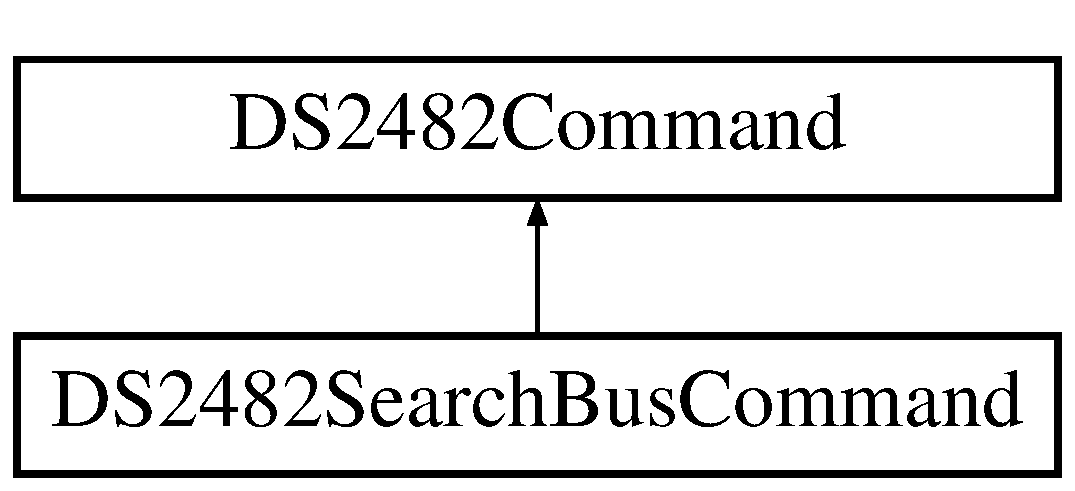
\includegraphics[height=2.000000cm]{class_d_s2482_search_bus_command}
\end{center}
\end{figure}
\subsection*{Public Member Functions}
\begin{DoxyCompactItemize}
\item 
\mbox{\hyperlink{class_d_s2482_device_list}{D\+S2482\+Device\+List}} \& \mbox{\hyperlink{class_d_s2482_search_bus_command_acf9ce76a212b1a927180ba4391a90f54}{get\+Device\+List}} ()
\begin{DoxyCompactList}\small\item\em Get the device list that was passed into run. \end{DoxyCompactList}\item 
\mbox{\Hypertarget{class_d_s2482_search_bus_command_a7425f532612d42aa2685597085f8a27f}\label{class_d_s2482_search_bus_command_a7425f532612d42aa2685597085f8a27f}} 
const \mbox{\hyperlink{class_d_s2482_device_list}{D\+S2482\+Device\+List}} \& \mbox{\hyperlink{class_d_s2482_search_bus_command_a7425f532612d42aa2685597085f8a27f}{get\+Device\+List}} () const
\begin{DoxyCompactList}\small\item\em Get the device list that was passed into run a const object. \end{DoxyCompactList}\end{DoxyCompactItemize}
\subsection*{Static Public Member Functions}
\begin{DoxyCompactItemize}
\item 
static \mbox{\hyperlink{class_d_s2482_search_bus_command}{D\+S2482\+Search\+Bus\+Command}} \& \mbox{\hyperlink{class_d_s2482_search_bus_command_ad45cdd2c6e517f13cf18bd28e58061bb}{run}} (\mbox{\hyperlink{class_d_s2482}{D\+S2482}} \&\mbox{\hyperlink{class_d_s2482_command_a54a41fb8a610ef2077f5e5377771aaf3}{parent}}, \mbox{\hyperlink{class_d_s2482_device_list}{D\+S2482\+Device\+List}} \&device\+List, std\+::function$<$ void(\mbox{\hyperlink{class_d_s2482_search_bus_command}{D\+S2482\+Search\+Bus\+Command}} \&, int status)$>$ completion)
\begin{DoxyCompactList}\small\item\em Run a D\+S18\+B20 search bus command to find all of the D\+S18\+B20s on the 1-\/wire bus. \end{DoxyCompactList}\end{DoxyCompactItemize}
\subsection*{Friends}
\begin{DoxyCompactItemize}
\item 
\mbox{\Hypertarget{class_d_s2482_search_bus_command_afeaf69274324e8dbeebede05c02d9c18}\label{class_d_s2482_search_bus_command_afeaf69274324e8dbeebede05c02d9c18}} 
class {\bfseries D\+S2482}
\end{DoxyCompactItemize}
\subsection*{Additional Inherited Members}


\subsection{Detailed Description}
Finds all of the devices on the 1-\/wire bus. 

If you have a multi-\/drop D\+S18\+B20 setup, this will find the 64-\/bit device addresses for every sensor on the 1-\/wire bus.

Searching the 1-\/wire bus temporarily requires about 800 bytes of heap space for the duration of the search.

As with all command objects, you do not typically construct one of these objects. Instead, use the static run method to handle allocating, initializing, and queueing the command. 

\subsection{Member Function Documentation}
\mbox{\Hypertarget{class_d_s2482_search_bus_command_acf9ce76a212b1a927180ba4391a90f54}\label{class_d_s2482_search_bus_command_acf9ce76a212b1a927180ba4391a90f54}} 
\index{D\+S2482\+Search\+Bus\+Command@{D\+S2482\+Search\+Bus\+Command}!get\+Device\+List@{get\+Device\+List}}
\index{get\+Device\+List@{get\+Device\+List}!D\+S2482\+Search\+Bus\+Command@{D\+S2482\+Search\+Bus\+Command}}
\subsubsection{\texorpdfstring{get\+Device\+List()}{getDeviceList()}}
{\footnotesize\ttfamily \mbox{\hyperlink{class_d_s2482_device_list}{D\+S2482\+Device\+List}}\& D\+S2482\+Search\+Bus\+Command\+::get\+Device\+List (\begin{DoxyParamCaption}{ }\end{DoxyParamCaption})\hspace{0.3cm}{\ttfamily [inline]}}



Get the device list that was passed into run. 

You can use this from the completion, however it\textquotesingle{}s not usually necessary since in most cases you\textquotesingle{}ll be able to access the variable you originally passed to run from your capture. But if for some reason you don\textquotesingle{}t want to capture it, you can use this. \mbox{\Hypertarget{class_d_s2482_search_bus_command_ad45cdd2c6e517f13cf18bd28e58061bb}\label{class_d_s2482_search_bus_command_ad45cdd2c6e517f13cf18bd28e58061bb}} 
\index{D\+S2482\+Search\+Bus\+Command@{D\+S2482\+Search\+Bus\+Command}!run@{run}}
\index{run@{run}!D\+S2482\+Search\+Bus\+Command@{D\+S2482\+Search\+Bus\+Command}}
\subsubsection{\texorpdfstring{run()}{run()}}
{\footnotesize\ttfamily \mbox{\hyperlink{class_d_s2482_search_bus_command}{D\+S2482\+Search\+Bus\+Command}} \& D\+S2482\+Search\+Bus\+Command\+::run (\begin{DoxyParamCaption}\item[{\mbox{\hyperlink{class_d_s2482}{D\+S2482}} \&}]{parent,  }\item[{\mbox{\hyperlink{class_d_s2482_device_list}{D\+S2482\+Device\+List}} \&}]{device\+List,  }\item[{std\+::function$<$ void(\mbox{\hyperlink{class_d_s2482_search_bus_command}{D\+S2482\+Search\+Bus\+Command}} \&, int status)$>$}]{completion }\end{DoxyParamCaption})\hspace{0.3cm}{\ttfamily [static]}}



Run a D\+S18\+B20 search bus command to find all of the D\+S18\+B20s on the 1-\/wire bus. 


\begin{DoxyParams}{Parameters}
{\em parent} & The \mbox{\hyperlink{class_d_s2482}{D\+S2482}} you want to send the command to. If it\textquotesingle{}s a D\+S2482\+\_\+800, make sure you set the channel as well.\\
\hline
{\em device\+List} & The \mbox{\hyperlink{class_d_s2482_device_list}{D\+S2482\+Device\+List}} object you want to save the list of devices to. The object is cleared before use.\\
\hline
{\em completion} & The completion handler lambda function. status is the result status of the call; if \mbox{\hyperlink{class_d_s2482_command_a8ffcf84807c97928dbfc61d75788e32b}{D\+S2482\+Command\+::\+R\+E\+S\+U\+L\+T\+\_\+\+D\+O\+NE}} then the call succeeded. If it\textquotesingle{}s any other value an error occurred.\\
\hline
\end{DoxyParams}
This call executes asynchronously. The completion function is called when complete or an error occurs. 

The documentation for this class was generated from the following files\+:\begin{DoxyCompactItemize}
\item 
src/D\+S2482-\/\+R\+K.\+h\item 
src/D\+S2482-\/\+R\+K.\+cpp\end{DoxyCompactItemize}

\hypertarget{class_d_s2482_search_rom}{}\section{D\+S2482\+Search\+Rom Class Reference}
\label{class_d_s2482_search_rom}\index{D\+S2482\+Search\+Rom@{D\+S2482\+Search\+Rom}}


Low-\/level class to send a S\+E\+A\+R\+C\+H\+\_\+\+R\+OM command. Normally you\textquotesingle{}d use \mbox{\hyperlink{class_d_s2482_search_bus_command}{D\+S2482\+Search\+Bus\+Command}} instead.  




{\ttfamily \#include $<$D\+S2482-\/\+R\+K.\+h$>$}

Inheritance diagram for D\+S2482\+Search\+Rom\+:\begin{figure}[H]
\begin{center}
\leavevmode
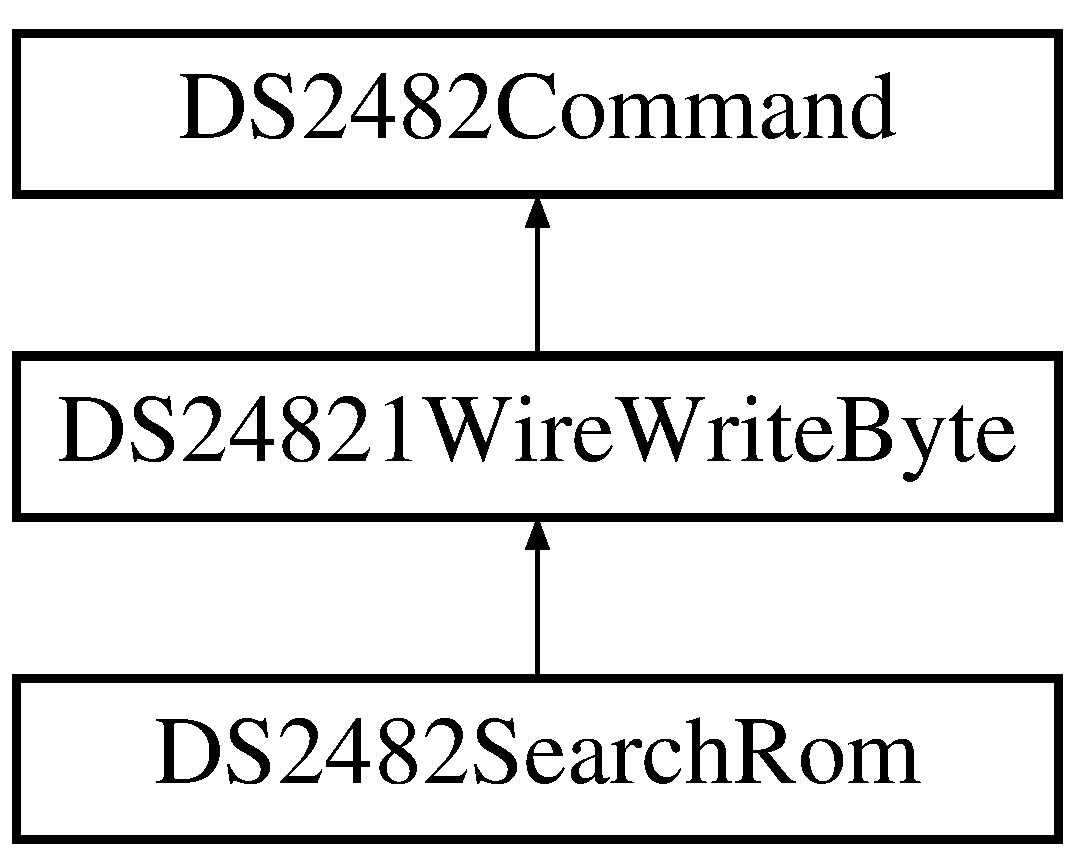
\includegraphics[height=3.000000cm]{class_d_s2482_search_rom}
\end{center}
\end{figure}
\subsection*{Static Public Member Functions}
\begin{DoxyCompactItemize}
\item 
\mbox{\Hypertarget{class_d_s2482_search_rom_aae9ecbe1d0b5e5dac6a38f1c4a2090f8}\label{class_d_s2482_search_rom_aae9ecbe1d0b5e5dac6a38f1c4a2090f8}} 
static \mbox{\hyperlink{class_d_s2482_search_rom}{D\+S2482\+Search\+Rom}} \& \mbox{\hyperlink{class_d_s2482_search_rom_aae9ecbe1d0b5e5dac6a38f1c4a2090f8}{run}} (\mbox{\hyperlink{class_d_s2482}{D\+S2482}} \&\mbox{\hyperlink{class_d_s2482_command_a54a41fb8a610ef2077f5e5377771aaf3}{parent}}, std\+::function$<$ void(\mbox{\hyperlink{class_d_s24821_wire_write_byte}{D\+S24821\+Wire\+Write\+Byte}} \&, int status)$>$ completion)
\begin{DoxyCompactList}\small\item\em Sends a S\+E\+A\+R\+C\+H\+\_\+\+R\+OM command -\/ used internally. \end{DoxyCompactList}\end{DoxyCompactItemize}
\subsection*{Friends}
\begin{DoxyCompactItemize}
\item 
\mbox{\Hypertarget{class_d_s2482_search_rom_afeaf69274324e8dbeebede05c02d9c18}\label{class_d_s2482_search_rom_afeaf69274324e8dbeebede05c02d9c18}} 
class {\bfseries D\+S2482}
\end{DoxyCompactItemize}
\subsection*{Additional Inherited Members}


\subsection{Detailed Description}
Low-\/level class to send a S\+E\+A\+R\+C\+H\+\_\+\+R\+OM command. Normally you\textquotesingle{}d use \mbox{\hyperlink{class_d_s2482_search_bus_command}{D\+S2482\+Search\+Bus\+Command}} instead. 

As with all command objects, you do not typically construct one of these objects. Instead, use the static run method to handle allocating, initializing, and queueing the command. 

The documentation for this class was generated from the following files\+:\begin{DoxyCompactItemize}
\item 
src/D\+S2482-\/\+R\+K.\+h\item 
src/D\+S2482-\/\+R\+K.\+cpp\end{DoxyCompactItemize}

\hypertarget{class_d_s2482_set_config_command}{}\section{D\+S2482\+Set\+Config\+Command Class Reference}
\label{class_d_s2482_set_config_command}\index{D\+S2482\+Set\+Config\+Command@{D\+S2482\+Set\+Config\+Command}}


Sets the configuration for a device.  




{\ttfamily \#include $<$D\+S2482-\/\+R\+K.\+h$>$}

Inheritance diagram for D\+S2482\+Set\+Config\+Command\+:\begin{figure}[H]
\begin{center}
\leavevmode
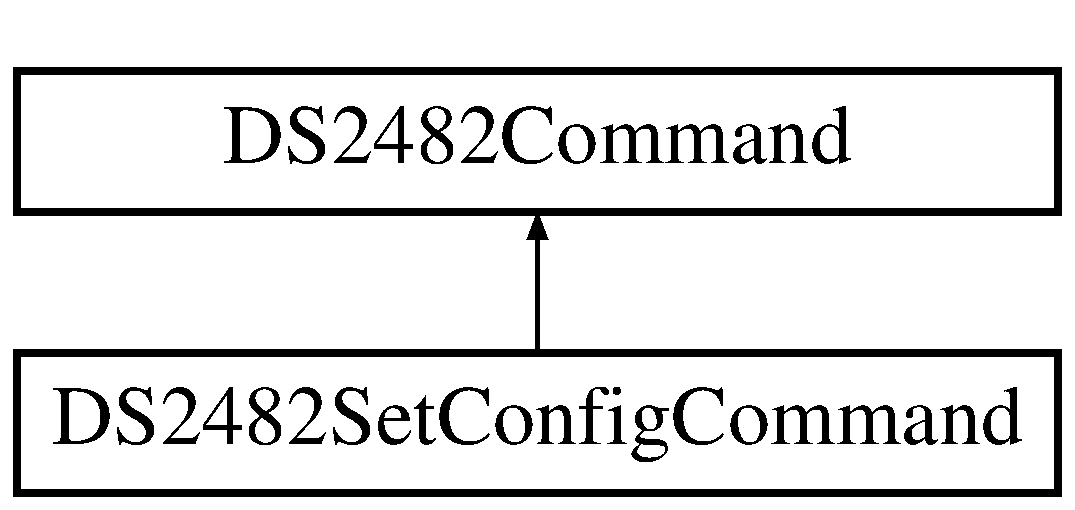
\includegraphics[height=2.000000cm]{class_d_s2482_set_config_command}
\end{center}
\end{figure}
\subsection*{Public Member Functions}
\begin{DoxyCompactItemize}
\item 
\mbox{\hyperlink{class_d_s2482_set_config_command}{D\+S2482\+Set\+Config\+Command}} \& \mbox{\hyperlink{class_d_s2482_set_config_command_a9c1f96c1cb321f98970df4ef12bd97a7}{with\+Parasitic\+Power}} (bool value=true)
\item 
\mbox{\hyperlink{class_d_s2482_set_config_command}{D\+S2482\+Set\+Config\+Command}} \& \mbox{\hyperlink{class_d_s2482_set_config_command_a90b06127e4a7f88a3f4b4a69546f6e53}{with\+TL}} (int8\+\_\+t value)
\item 
\mbox{\hyperlink{class_d_s2482_set_config_command}{D\+S2482\+Set\+Config\+Command}} \& \mbox{\hyperlink{class_d_s2482_set_config_command_aab39af606ba1bf9a00e05129c7bd4fc9}{with\+TH}} (int8\+\_\+t value)
\end{DoxyCompactItemize}
\subsection*{Static Public Member Functions}
\begin{DoxyCompactItemize}
\item 
static \mbox{\hyperlink{class_d_s2482_set_config_command}{D\+S2482\+Set\+Config\+Command}} \& \mbox{\hyperlink{class_d_s2482_set_config_command_afbf596cbb1c6e8f5d97918aa54946d2f}{run}} (\mbox{\hyperlink{class_d_s2482}{D\+S2482}} \&\mbox{\hyperlink{class_d_s2482_command_a54a41fb8a610ef2077f5e5377771aaf3}{parent}}, \mbox{\hyperlink{class_d_s2482_device_list}{D\+S2482\+Device\+List}} \&device\+List, bool save\+To\+E\+E\+P\+R\+OM, int conversion\+Size, std\+::function$<$ void(\mbox{\hyperlink{class_d_s2482_set_config_command}{D\+S2482\+Set\+Config\+Command}} \&, int status)$>$ completion)
\begin{DoxyCompactList}\small\item\em Run a D\+S18\+B20 set configuration command to set D\+S18\+B20 configuration. \end{DoxyCompactList}\end{DoxyCompactItemize}
\subsection*{Friends}
\begin{DoxyCompactItemize}
\item 
\mbox{\Hypertarget{class_d_s2482_set_config_command_afeaf69274324e8dbeebede05c02d9c18}\label{class_d_s2482_set_config_command_afeaf69274324e8dbeebede05c02d9c18}} 
class {\bfseries D\+S2482}
\end{DoxyCompactItemize}
\subsection*{Additional Inherited Members}


\subsection{Detailed Description}
Sets the configuration for a device. 

Normally this is done to change the number of bits of conversion precision. It can be used for the alarm feature as well, but alarm is not supported by this library because the operation is a little strange and I\textquotesingle{}m not really convinced that it\textquotesingle{}s that useful.

As with all command objects, you do not typically construct one of these objects. Instead, use the static run method to handle allocating, initializing, and queueing the command. 

\subsection{Member Function Documentation}
\mbox{\Hypertarget{class_d_s2482_set_config_command_afbf596cbb1c6e8f5d97918aa54946d2f}\label{class_d_s2482_set_config_command_afbf596cbb1c6e8f5d97918aa54946d2f}} 
\index{D\+S2482\+Set\+Config\+Command@{D\+S2482\+Set\+Config\+Command}!run@{run}}
\index{run@{run}!D\+S2482\+Set\+Config\+Command@{D\+S2482\+Set\+Config\+Command}}
\subsubsection{\texorpdfstring{run()}{run()}}
{\footnotesize\ttfamily \mbox{\hyperlink{class_d_s2482_set_config_command}{D\+S2482\+Set\+Config\+Command}} \& D\+S2482\+Set\+Config\+Command\+::run (\begin{DoxyParamCaption}\item[{\mbox{\hyperlink{class_d_s2482}{D\+S2482}} \&}]{parent,  }\item[{\mbox{\hyperlink{class_d_s2482_device_list}{D\+S2482\+Device\+List}} \&}]{device\+List,  }\item[{bool}]{save\+To\+E\+E\+P\+R\+OM,  }\item[{int}]{conversion\+Size,  }\item[{std\+::function$<$ void(\mbox{\hyperlink{class_d_s2482_set_config_command}{D\+S2482\+Set\+Config\+Command}} \&, int status)$>$}]{completion }\end{DoxyParamCaption})\hspace{0.3cm}{\ttfamily [static]}}



Run a D\+S18\+B20 set configuration command to set D\+S18\+B20 configuration. 


\begin{DoxyParams}{Parameters}
{\em parent} & The \mbox{\hyperlink{class_d_s2482}{D\+S2482}} you want to send the command to. If it\textquotesingle{}s a D\+S2482\+\_\+800, make sure you set the channel as well.\\
\hline
{\em device\+List} & The list of devices you want to set the configuration on.\\
\hline
{\em save\+To\+E\+E\+P\+R\+OM} & Saves the configuration settings to E\+E\+P\+R\+OM so they will be reused when power is reset.\\
\hline
{\em conversion\+Size} & The number of bits of conversion to do. The constants are defined in the \mbox{\hyperlink{class_d_s2482_command}{D\+S2482\+Command}} class and are one of\+: C\+O\+N\+V\+E\+R\+S\+I\+O\+N\+\_\+9\+B\+IT, C\+O\+N\+V\+E\+R\+S\+I\+O\+N\+\_\+10\+B\+IT, C\+O\+N\+V\+E\+R\+S\+I\+O\+N\+\_\+11\+B\+IT, or C\+O\+N\+V\+E\+R\+S\+I\+O\+N\+\_\+12\+B\+IT. At 9 bits, the resolution is 1/2 degrees C. At 12 bits, the resolution is 1/16 degrees C. The factory default hardware setting is 12 bits.\\
\hline
{\em completion} & The completion handler lambda function. status is the result status of the call; if \mbox{\hyperlink{class_d_s2482_command_a8ffcf84807c97928dbfc61d75788e32b}{D\+S2482\+Command\+::\+R\+E\+S\+U\+L\+T\+\_\+\+D\+O\+NE}} then the call succeeded. If it\textquotesingle{}s any other value an error occurred.\\
\hline
\end{DoxyParams}
\begin{DoxyReturn}{Returns}
The new configuration object so you can use the optional settings like with\+Parasitic\+Power, fluent-\/style.
\end{DoxyReturn}
Reducing the resolution reduces the amount of time to capture the current temperature (ConvertT)\+:

\tabulinesep=1mm
\begin{longtabu} spread 0pt [c]{*{2}{|X[-1]}|}
\hline
\rowcolor{\tableheadbgcolor}\textbf{ Bits  }&\textbf{ Time (milliseconds)   }\\\cline{1-2}
\endfirsthead
\hline
\endfoot
\hline
\rowcolor{\tableheadbgcolor}\textbf{ Bits  }&\textbf{ Time (milliseconds)   }\\\cline{1-2}
\endhead
9  &94   \\\cline{1-2}
10  &188   \\\cline{1-2}
11  &375   \\\cline{1-2}
12  &750   \\\cline{1-2}
\end{longtabu}


It doesn\textquotesingle{}t affect the amount of data transmitted by the sensors; that\textquotesingle{}s always 9 bytes, regardless of resolution.

This call executes asynchronously. The completion function is called when complete or an error occurs. \mbox{\Hypertarget{class_d_s2482_set_config_command_a9c1f96c1cb321f98970df4ef12bd97a7}\label{class_d_s2482_set_config_command_a9c1f96c1cb321f98970df4ef12bd97a7}} 
\index{D\+S2482\+Set\+Config\+Command@{D\+S2482\+Set\+Config\+Command}!with\+Parasitic\+Power@{with\+Parasitic\+Power}}
\index{with\+Parasitic\+Power@{with\+Parasitic\+Power}!D\+S2482\+Set\+Config\+Command@{D\+S2482\+Set\+Config\+Command}}
\subsubsection{\texorpdfstring{with\+Parasitic\+Power()}{withParasiticPower()}}
{\footnotesize\ttfamily \mbox{\hyperlink{class_d_s2482_set_config_command}{D\+S2482\+Set\+Config\+Command}}\& D\+S2482\+Set\+Config\+Command\+::with\+Parasitic\+Power (\begin{DoxyParamCaption}\item[{bool}]{value = {\ttfamily true} }\end{DoxyParamCaption})\hspace{0.3cm}{\ttfamily [inline]}}

Sets whether to use parasitic power or not. The default is false. \mbox{\Hypertarget{class_d_s2482_set_config_command_aab39af606ba1bf9a00e05129c7bd4fc9}\label{class_d_s2482_set_config_command_aab39af606ba1bf9a00e05129c7bd4fc9}} 
\index{D\+S2482\+Set\+Config\+Command@{D\+S2482\+Set\+Config\+Command}!with\+TH@{with\+TH}}
\index{with\+TH@{with\+TH}!D\+S2482\+Set\+Config\+Command@{D\+S2482\+Set\+Config\+Command}}
\subsubsection{\texorpdfstring{with\+T\+H()}{withTH()}}
{\footnotesize\ttfamily \mbox{\hyperlink{class_d_s2482_set_config_command}{D\+S2482\+Set\+Config\+Command}}\& D\+S2482\+Set\+Config\+Command\+::with\+TH (\begin{DoxyParamCaption}\item[{int8\+\_\+t}]{value }\end{DoxyParamCaption})\hspace{0.3cm}{\ttfamily [inline]}}

Set the TH value, the hugh temperature alarm, which can also be used as an arbitrarary 8-\/bit value stored in E\+E\+P\+R\+OM. \mbox{\Hypertarget{class_d_s2482_set_config_command_a90b06127e4a7f88a3f4b4a69546f6e53}\label{class_d_s2482_set_config_command_a90b06127e4a7f88a3f4b4a69546f6e53}} 
\index{D\+S2482\+Set\+Config\+Command@{D\+S2482\+Set\+Config\+Command}!with\+TL@{with\+TL}}
\index{with\+TL@{with\+TL}!D\+S2482\+Set\+Config\+Command@{D\+S2482\+Set\+Config\+Command}}
\subsubsection{\texorpdfstring{with\+T\+L()}{withTL()}}
{\footnotesize\ttfamily \mbox{\hyperlink{class_d_s2482_set_config_command}{D\+S2482\+Set\+Config\+Command}}\& D\+S2482\+Set\+Config\+Command\+::with\+TL (\begin{DoxyParamCaption}\item[{int8\+\_\+t}]{value }\end{DoxyParamCaption})\hspace{0.3cm}{\ttfamily [inline]}}

Set the TL value, the low temperature alarm, which can also be used as an arbitrarary 8-\/bit value stored in E\+E\+P\+R\+OM. 

The documentation for this class was generated from the following files\+:\begin{DoxyCompactItemize}
\item 
src/D\+S2482-\/\+R\+K.\+h\item 
src/D\+S2482-\/\+R\+K.\+cpp\end{DoxyCompactItemize}

\hypertarget{class_d_s2482_skip_rom}{}\section{D\+S2482\+Skip\+Rom Class Reference}
\label{class_d_s2482_skip_rom}\index{D\+S2482\+Skip\+Rom@{D\+S2482\+Skip\+Rom}}


Low-\/level class to send a S\+K\+I\+P\+\_\+\+R\+OM command. This is used internally by D\+S2482\+Read\+Scratchpad and others.  




{\ttfamily \#include $<$D\+S2482-\/\+R\+K.\+h$>$}

Inheritance diagram for D\+S2482\+Skip\+Rom\+:\begin{figure}[H]
\begin{center}
\leavevmode
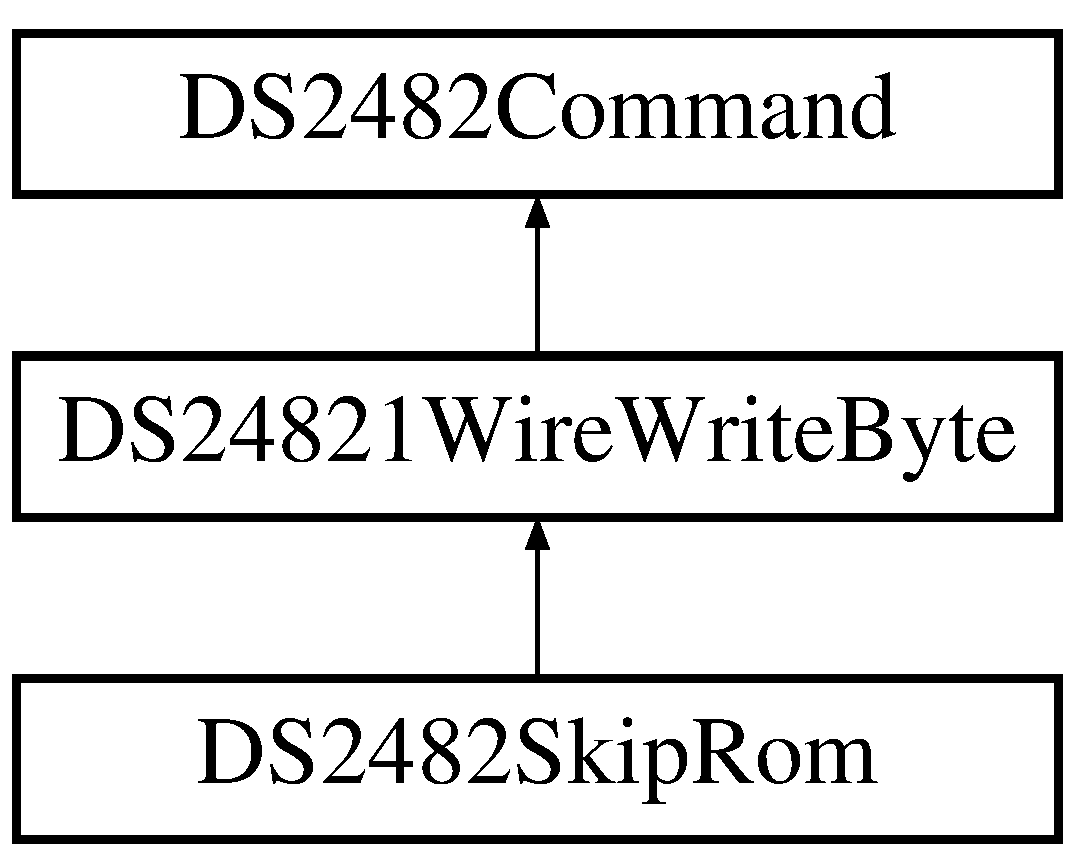
\includegraphics[height=3.000000cm]{class_d_s2482_skip_rom}
\end{center}
\end{figure}
\subsection*{Static Public Member Functions}
\begin{DoxyCompactItemize}
\item 
\mbox{\Hypertarget{class_d_s2482_skip_rom_a83c24bab7c454912e818aeacba765588}\label{class_d_s2482_skip_rom_a83c24bab7c454912e818aeacba765588}} 
static \mbox{\hyperlink{class_d_s2482_skip_rom}{D\+S2482\+Skip\+Rom}} \& \mbox{\hyperlink{class_d_s2482_skip_rom_a83c24bab7c454912e818aeacba765588}{run}} (\mbox{\hyperlink{class_d_s2482}{D\+S2482}} \&\mbox{\hyperlink{class_d_s2482_command_a54a41fb8a610ef2077f5e5377771aaf3}{parent}}, std\+::function$<$ void(\mbox{\hyperlink{class_d_s24821_wire_write_byte}{D\+S24821\+Wire\+Write\+Byte}} \&, int status)$>$ completion)
\begin{DoxyCompactList}\small\item\em Sends a S\+K\+I\+P\+\_\+\+R\+OM command -\/ used internally. \end{DoxyCompactList}\end{DoxyCompactItemize}
\subsection*{Friends}
\begin{DoxyCompactItemize}
\item 
\mbox{\Hypertarget{class_d_s2482_skip_rom_afeaf69274324e8dbeebede05c02d9c18}\label{class_d_s2482_skip_rom_afeaf69274324e8dbeebede05c02d9c18}} 
class {\bfseries D\+S2482}
\end{DoxyCompactItemize}
\subsection*{Additional Inherited Members}


\subsection{Detailed Description}
Low-\/level class to send a S\+K\+I\+P\+\_\+\+R\+OM command. This is used internally by D\+S2482\+Read\+Scratchpad and others. 

As with all command objects, you do not typically construct one of these objects. Instead, use the static run method to handle allocating, initializing, and queueing the command. 

The documentation for this class was generated from the following files\+:\begin{DoxyCompactItemize}
\item 
src/D\+S2482-\/\+R\+K.\+h\item 
src/D\+S2482-\/\+R\+K.\+cpp\end{DoxyCompactItemize}

%--- End generated contents ---

% Index
\backmatter
\newpage
\phantomsection
\clearemptydoublepage
\addcontentsline{toc}{chapter}{Index}
\printindex

\end{document}
